\documentclass[11pt]{report}
\usepackage[a4paper, tmargin=0.75in, lmargin=0.80in, rmargin=0.80in, bmargin=1in]{geometry}
\usepackage{fontspec}
\usepackage{polyglossia}
\setdefaultlanguage{greek}
\setmainfont{GFS Didot}
\newfontfamily\greekfont{GFS Didot}
\usepackage{float}
\newfontfamily\greekfonttt{FreeMono} 
\setmonofont{FreeMono}
\usepackage{tcolorbox}
\tcbuselibrary{listingsutf8}

\usepackage{titlesec}
\usepackage{graphicx}
\graphicspath{{figures/}}

\usepackage{hyperref}
\hypersetup{
    colorlinks=true,
    linkcolor=blue,
    filecolor=magenta,      
    urlcolor=blue,
    citecolor=black,
    linktoc=all
}

\newcommand{\studentname}{Ματίνα Παπαδάκου: Π21127 \\ Φωτιάδης Δημήτριος: Π21183 \\ 
Καλαμάρα Γλυκερία: Π21042}
\newcommand{\projecttitle}{Εκπαιδευτικό Λογισμικό}
\newcommand{\supervisorA}{Αριστέα Κοντογιάννη}
\newcommand{\university}{Πανεπιστήμιο Πειραιά}
\newcommand{\school}{Σχολή Τεχνολογιών Πληροφορικής και Επικοινωνιών}

\begin{document}

\begin{titlepage}
    \begin{center}

\includegraphics[width=0.5\linewidth]{Figures/papei.jpg}
        \vspace{0.5cm}
        \rule{15cm}{2.5pt} \\
        \textbf{\Huge \projecttitle} \\
        \rule{15cm}{2.5pt}
        
        \vspace{1cm}
        \textbf{\Large Απαλλακτική Εργασία με τίτλο: "PyLearn - Μαθαίνω Python στο
Λύκειο" \\}

        \vspace{0.5cm}
        από
        
        \vspace{0.5cm}
        \textbf{\LARGE \studentname} \\
        
        \vspace{0.8cm}
        \school \\
        \university
        
        \vspace{1.5cm}
        \textbf{\large Επιβλέπουσα Καθηγήτρια} \\
        \supervisorA
        
        \vspace{2.5cm}
        \textbf{\large Ημερομηνία: 28 Μαΐου 2025}
    \end{center}
\end{titlepage}

\pagenumbering{roman}
\tableofcontents
\clearpage
\pagenumbering{arabic}

\chapter{Περιγραφή Εργασίας}

Η παρούσα εργασία αφορά την ανάλυση, σχεδίαση και ανάπτυξη ενός εκπαιδευτικού λογισμικού με σκοπό τη διδασκαλία της γλώσσας προγραμματισμού Python σε μαθητές Λυκείου. Ο στόχος είναι η ενίσχυση της γνώσης και του ενδιαφέροντος των μαθητών για τον προγραμματισμό, μέσα από ένα διαδραστικό, φιλικό προς τον χρήστη και ακαδημαϊκά τεκμηριωμένο περιβάλλον μάθησης. 

Η επιλογή της γλώσσας Python ως βασικού αντικειμένου διδασκαλίας έγινε με βάση τη δημοφιλία, την απλότητα σύνταξης και την ευρεία χρήση της σε επιστημονικά, επαγγελματικά και εκπαιδευτικά πεδία. Η Python αποτελεί ιδανική επιλογή για την εισαγωγή στον προγραμματισμό, καθώς συνδυάζει την ισχύ και την ευελιξία με την κατανοητή και σαφή σύνταξη, διευκολύνοντας τους αρχάριους προγραμματιστές να επικεντρωθούν στις λογικές δομές και την αλγοριθμική σκέψη χωρίς να αποθαρρύνονται από τεχνικές λεπτομέρειες. 

Η εργασία αποσκοπεί στην ανάπτυξη ενός εκπαιδευτικού λογισμικού το οποίο δομείται σε διακριτές ενότητες διδασκαλίας, καθεμία εκ των οποίων περιλαμβάνει θεωρητικό περιεχόμενο, παραδείγματα κώδικα, ασκήσεις και τεστ αυτοαξιολόγησης. Η εφαρμογή αξιοποιεί τεχνικές πολυτροπικής μάθησης, παρέχοντας συνδυασμό κειμένου, οπτικού υλικού (π.χ. βίντεο) και διαδραστικών δραστηριοτήτων (π.χ. drag and drop, συμπλήρωση κενού). Παράλληλα, ενσωματώνεται σύστημα καταγραφής προόδου και προσαρμοσμένης μάθησης, το οποίο επιτρέπει την εξατομίκευση του μαθησιακού μονοπατιού με βάση την απόδοση και τα λάθη του χρήστη. 

Η εφαρμογή υποστηρίζεται τεχνικά από ένα συνδυασμό τεχνολογιών frontend και backend, ενώ τα δεδομένα χρήστη αποθηκεύονται σε μη σχεσιακή βάση δεδομένων εξασφαλίζοντας παρακολούθηση της αλληλεπίδρασης και στατιστική επεξεργασία των αποτελεσμάτων. 

Τέλος, η εργασία ακολουθεί οργανωμένη μεθοδολογία ανάπτυξης λογισμικού: ξεκινώντας από την ανάλυση των εκπαιδευτικών αναγκών και των απαιτήσεων του τελικού χρήστη, προχωρά στη χαρτογράφηση των στόχων διδασκαλίας, τη σχεδίαση της αρχιτεκτονικής της εφαρμογής και την υλοποίηση του περιβάλλοντος μάθησης.

\chapter{Ανάλυση Απαιτήσεων}
\section{Εκπαιδευτικές Ανάγκες}

Η ανάπτυξη του εκπαιδευτικού λογισμικού βασίστηκε στην αναγνώριση συγκεκριμένων εκπαιδευτικών αναγκών που αφορούν τη διδασκαλία του προγραμματισμού σε μαθητές Λυκείου. Στο σύγχρονο ψηφιακό περιβάλλον, η ικανότητα προγραμματιστικής σκέψης και η εξοικείωση με βασικές γλώσσες προγραμματισμού θεωρούνται θεμελιώδεις δεξιότητες. Ωστόσο, η εισαγωγή αυτών των εννοιών στην τάξη συχνά αντιμετωπίζει προκλήσεις, όπως η έλλειψη εξειδικευμένου εξοπλισμού, η ανομοιογένεια του μαθητικού πληθυσμού ως προς τις γνώσεις, αλλά και η δυσκολία ενεργοποίησης του ενδιαφέροντος των μαθητών.

Προκειμένου να καλυφθούν οι παραπάνω ανάγκες, το λογισμικό αναπτύχθηκε με γνώμονα τα εξής:

\begin{itemize}
    \item \textbf{Προσβασιμότητα:} Η εφαρμογή λειτουργεί σε φορητές συσκευές Android, γεγονός που επιτρέπει τη χρήση της εντός και εκτός σχολικού περιβάλλοντος, χωρίς την απαίτηση υπολογιστών ή εξειδικευμένων εργαστηρίων πληροφορικής.
    
    \item \textbf{Απλοποίηση πολύπλοκων εννοιών:} Μέσω πολυμεσικού και διαδραστικού υλικού (π.χ. κουίζ, κώδικας με λάθη, drag \& drop), οι αφηρημένες έννοιες του προγραμματισμού μετατρέπονται σε κατανοητές, χειροπιαστές δραστηριότητες.
    
    \item \textbf{Ανάπτυξη δεξιοτήτων αυτορρυθμιζόμενης μάθησης:} Η εφαρμογή ενσωματώνει αυτοαξιολόγηση, ανατροφοδότηση και προσαρμοσμένες διαδρομές μάθησης, ενισχύοντας την αυτονομία του μαθητή.
    
    \item \textbf{Συμμόρφωση με το Αναλυτικό Πρόγραμμα Σπουδών Πληροφορικής:} Οι ενότητες του λογισμικού χαρτογραφούνται στις βασικές δεξιότητες που προβλέπονται για την κατανόηση και χρήση γλωσσών προγραμματισμού στο Γενικό Λύκειο.
\end{itemize}

Συνεπώς, η εφαρμογή στοχεύει όχι μόνο στη μετάδοση γνώσης, αλλά και στην αλλαγή της στάσης των μαθητών απέναντι στον προγραμματισμό, προωθώντας την ενεργό συμμετοχή, την ανακαλυπτική μάθηση και την κριτική σκέψη.

\section{Ανάλυση Χρηστών (Μαθητές)}

Οι βασικοί χρήστες της παρούσας εκπαιδευτικής εφαρμογής είναι μαθητές Λυκείου, ηλικίας μεταξύ 15 και 18 ετών, οι οποίοι είτε βρίσκονται στο αρχικό στάδιο της επαφής τους με τον προγραμματισμό είτε διαθέτουν μόνο επιφανειακές γνώσεις. Το κοινό αυτό χαρακτηρίζεται από γνωστική ετερογένεια, καθώς περιλαμβάνει μαθητές με διαφορετικό βαθμό εξοικείωσης με τις τεχνολογίες, ανομοιογενές μαθησιακό προφίλ και ποικίλα κίνητρα συμμετοχής. Η κατανόηση των χαρακτηριστικών των μαθητών αποτέλεσε βασικό στοιχείο κατά τη φάση του σχεδιασμού της εφαρμογής, επηρεάζοντας τόσο τη διεπαφή όσο και τη διαβάθμιση και μορφή του διδακτικού περιεχομένου. 

Οι μαθητές, κατά κανόνα, δεν έχουν συστηματική εμπειρία στην ανάπτυξη κώδικα ή στην αλγοριθμική σκέψη. Η διαδικασία μάθησης του προγραμματισμού συχνά προκαλεί γνωστική επιβάρυνση, λόγω της ανάγκης παρακολούθησης της λογικής ροής και των αφηρημένων εννοιών. Για τον λόγο αυτό, κρίθηκε απαραίτητο η εφαρμογή να υιοθετήσει σταδιακή και προοδευτική προσέγγιση παρουσίασης της πληροφορίας, ενισχυμένη με κατάλληλα παραδείγματα, απλουστευμένα σενάρια και ανατροφοδότηση που βασίζεται στη διαγνωστική αξιολόγηση. Ο σχεδιασμός των δραστηριοτήτων, επιπλέον, δίνει έμφαση στην ενεργητική εμπλοκή του μαθητή, μετατρέποντας την παθητική παρακολούθηση σε διαδραστική μάθηση. 

Αξιοποιώντας το γεγονός ότι οι μαθητές έχουν ιδιαίτερα υψηλό βαθμό εξοικείωσης με τις κινητές συσκευές και τις εφαρμογές Android, η υλοποίηση της εφαρμογής έγινε αποκλειστικά για φορητές συσκευές, με στόχο τη μείωση του φραγμού πρόσβασης και τη φυσική ενσωμάτωση της μάθησης στην καθημερινότητά τους. Η διεπαφή χρήστη σχεδιάστηκε με γνώμονα τη χρηστικότητα, την απλότητα και την οπτική ευκρίνεια, ώστε να είναι ελκυστική και λειτουργική ακόμη και για μαθητές με μικρή εμπειρία σε αντίστοιχα περιβάλλοντα. 

Τέλος, λήφθηκε υπόψη ότι οι μαθητές μαθαίνουν με διαφορετικούς ρυθμούς και στυλ, γεγονός που ενίσχυσε την ανάγκη για ενσωμάτωση στοιχείων εξατομικευμένης μάθησης. Η εφαρμογή, μέσω της σύνδεσης με το Firebase, παρακολουθεί και αποθηκεύει την πρόοδο κάθε χρήστη, προσαρμόζοντας το περιεχόμενο στις ανάγκες του. Οι μαθητές που αντιμετωπίζουν δυσκολίες λαμβάνουν ενισχυτικό υλικό και πιο απλές δραστηριότητες, ενώ εκείνοι που προοδεύουν ταχύτερα έχουν πρόσβαση σε πιο απαιτητικές προκλήσεις και mini projects. Αυτή η δυναμική προσαρμογή της μαθησιακής εμπειρίας διασφαλίζει τη συνεχή εμπλοκή και τη διατήρηση υψηλού επιπέδου ενδιαφέροντος. 
\section{Λειτουργικές \& Μη Λειτουργικές Απαιτήσεις}

Η επιτυχής υλοποίηση του εκπαιδευτικού λογισμικού προϋπέθεσε την αναγνώριση και τεκμηρίωση τόσο των λειτουργικών όσο και των μη λειτουργικών απαιτήσεων του συστήματος. Οι λειτουργικές απαιτήσεις αναφέρονται σε συγκεκριμένες λειτουργίες που πρέπει να εκτελεί η εφαρμογή, ώστε να εξυπηρετεί τους εκπαιδευτικούς της στόχους, ενώ οι μη λειτουργικές σχετίζονται με την ποιότητα, την απόδοση και τη συμπεριφορά του συστήματος κατά τη χρήση του. 

Σε επίπεδο λειτουργικών απαιτήσεων, η εφαρμογή όφειλε πρωτίστως να παρέχει τη δυνατότητα παρουσίασης εκπαιδευτικού περιεχομένου σε διακριτές ενότητες, οι οποίες να καλύπτουν σταδιακά τις βασικές έννοιες της γλώσσας Python. Κάθε ενότητα περιλαμβάνει θεωρητικά στοιχεία, παραδείγματα κώδικα, καθώς και αντίστοιχες ασκήσεις και δραστηριότητες αξιολόγησης. Απαραίτητη ήταν επίσης η δυνατότητα διαχείρισης διαδραστικών στοιχείων, όπως ερωτήσεις πολλαπλής επιλογής, συμπλήρωση κενού και δραστηριότητες τύπου drag and drop. Επιπλέον, η εφαρμογή έπρεπε να προσφέρει μηχανισμό καταγραφής της προόδου του μαθητή, ώστε να είναι δυνατή η εξατομίκευση της εκπαιδευτικής εμπειρίας μέσω προσαρμοστικών μηχανισμών. 

Στο πλαίσιο αυτό, κρίθηκε αναγκαία η σύνδεση με μία διαδικτυακή βάση δεδομένων (Firebase Realtime Database), μέσω της οποίας αποθηκεύονται δεδομένα σχετικά με τις επιδόσεις, τη συμπεριφορά πλοήγησης και τη συχνότητα αλληλεπίδρασης των μαθητών με την εφαρμογή. Το λογισμικό όφειλε επίσης να υποστηρίζει εγγραφή και είσοδο χρηστών (authentication), ώστε κάθε μαθητής να μπορεί να διατηρεί το προσωπικό του προφίλ και να συνεχίζει την εκμάθηση από το σημείο που είχε διακόψει. Ειδική πρόβλεψη έγινε για τη σταδιακή αποκάλυψη περιεχομένου με βάση την πρόοδο, προσφέροντας έναν μηχανισμό σταδιακής επιβράβευσης και ενίσχυσης του κινήτρου. 

Οι μη λειτουργικές απαιτήσεις αφορούσαν κυρίως την εμπειρία χρήσης, τη συμβατότητα, την ασφάλεια και την απόδοση της εφαρμογής. Πρώτιστη απαίτηση ήταν η εφαρμογή να λειτουργεί απρόσκοπτα σε φορητές συσκευές Android, ανεξαρτήτως μεγέθους οθόνης ή έκδοσης λειτουργικού συστήματος (εντός λογικών ορίων). Ιδιαίτερη έμφαση δόθηκε στη φιλικότητα του περιβάλλοντος χρήσης, με απλό, κατανοητό και καλαίσθητο σχεδιασμό διεπαφής, που να ενθαρρύνει την εξερεύνηση χωρίς να προκαλεί σύγχυση. Η ταχύτητα απόκρισης σε αλληλεπιδράσεις θεωρήθηκε κρίσιμη, καθώς η εκπαιδευτική αποτελεσματικότητα μειώνεται δραστικά όταν παρατηρούνται καθυστερήσεις ή τεχνικά σφάλματα κατά τη χρήση. 

Σε επίπεδο ασφάλειας, αν και το περιεχόμενο δεν απαιτεί διαχείριση ευαίσθητων προσωπικών δεδομένων, εξασφαλίστηκε ότι η σύνδεση με τη βάση δεδομένων γίνεται μέσω πιστοποιημένων κλειδιών πρόσβασης και ότι οι χρήστες δεν έχουν πρόσβαση σε στοιχεία άλλων λογαριασμών. Η αρχιτεκτονική client-server που ακολουθήθηκε διασφαλίζει τη διαχωρισμένη και ασφαλή διαχείριση του backend από την εφαρμογή του χρήστη. 

 
\section{Είδη Μάθησης που χρησιμοποιήθηκαν}

Η σχεδίαση της εφαρμογής στηρίζεται στην αξιοποίηση πολλαπλών παιδαγωγικών προσεγγίσεων μάθησης, οι οποίες εφαρμόζονται διαθεματικά σε όλο το εκπαιδευτικό περιεχόμενο, διαφοροποιούνται ανά ενότητα και ενεργοποιούνται δυναμικά ανάλογα με τις ανάγκες του μαθητή. Η επιλογή και η ενσωμάτωση των εκπαιδευτικών τύπων μάθησης δεν έγινε αυθαίρετα, αλλά στη βάση τεκμηριωμένων θεωριών μάθησης και με στόχο την ενεργοποίηση της γνωστικής, πρακτικής και ανακαλυπτικής διάστασης της εκπαίδευσης. Παρακάτω περιγράφονται αναλυτικά όλα τα είδη μάθησης που αξιοποιούνται στην πλατφόρμα, καθώς και η λειτουργική τους εφαρμογή ανά ενότητα. 

\subsection*{Προσαρμοσμένη Μάθηση (Adaptive Learning)}

Ο μηχανισμός προσαρμογής αποτελεί το δομικό πυρήνα των ενοτήτων. Για παράδειγμα, στην Ενότητα 1, σε περίπτωση αποτυχίας στο quiz, ο χρήστης παραπέμπεται σε επαναληπτικό υλικό ανάλογα με το μαθησιακό του προφίλ — συγκεκριμένα σε οπτικό υλικό (βίντεο) ή κειμενική ανακεφαλαίωση. Σε περίπτωση επιτυχίας, του προτείνεται προαιρετικό εμπλουτιστικό υλικό, όπως η παρουσίαση διάσημων εφαρμογών σε Python. Αντίστοιχα στην Ενότητα 2, η επιτυχία ξεκλειδώνει μια προαιρετική δημιουργική άσκηση, ενώ η αποτυχία οδηγεί σε ανακεφαλαιωτικά παραδείγματα και επαναφορά στη θεωρία.  

\subsection*{Γνωστική Μάθηση (Cognitive Learning) }

Η γνωστική μάθηση αφορά τη διαδικασία αφομοίωσης, κατανόησης και επεξεργασίας νέας πληροφορίας. Εμφανίζεται έντονα σε κάθε νέα θεματική ενότητα όπου εισάγεται θεωρητικό υπόβαθρο. Στην Ενότητα 3, για παράδειγμα, η επεξεργασία των δομών ελέγχου (if, elif, else) και των λογικών τελεστών απαιτεί εννοιολογική κατανόηση και σύνδεση με προϋπάρχουσες γνώσεις. Αντίστοιχα, στην Ενότητα 4, η κατανόηση των επαναλήψεων (for/while) και των λιστών αποτελεί καθαρή γνωστική λειτουργία. Η ίδια δομή διατηρείται και στην Ενότητα 5, με την εισαγωγή των συναρτήσεων. Σε όλα αυτά τα σημεία, ο μαθητής έρχεται σε επαφή με νέα σύμβολα, λογική δομή και συντακτικούς κανόνες, τους οποίους καλείται να κατανοήσει θεωρητικά προτού τους εφαρμόσει. 

\subsection*{Μάθηση μέσω Εξάσκησης (Practice-Based Learning) }

Η εφαρμογή ενσωματώνει πρακτική εξάσκηση ως βασικό εργαλείο εμπέδωσης. Στην Ενότητα 3, οι μαθητές εξασκούνται σε quiz πολλαπλής επιλογής και Drag and Drop ταξινόμησης εντολών, ενώ στην Ενότητα 4 εφαρμόζουν τη θεωρία γράφοντας επαναληπτικές δομές και επεξεργαζόμενοι λίστες. Στην Ενότητα 5, η χρήση συναρτήσεων μετατρέπεται σε πρακτική συνήθεια μέσω επαναλαμβανόμενων ασκήσεων. Μέσα από την εξάσκηση, οι μαθητές αναπτύσσουν ροή σκέψης, ενισχύουν τη συντακτική τους ακρίβεια και σταθεροποιούν τις γνώσεις τους με χειρισμό πραγματικών παραδειγμάτων. 

\subsection*{Μάθηση μέσω Λαθών (Error-Based Learning) }

Η μάθηση μέσω σφαλμάτων ενεργοποιείται σε πλήθος δραστηριοτήτων. Οι μαθητές καλούνται να εντοπίσουν και να διορθώσουν λάθη είτε συντακτικά είτε λογικά, αποκτώντας δεξιότητες παρατηρητικότητας, ενσυναίσθησης της ροής εκτέλεσης και εμβάθυνσης στη λειτουργική σημασία κάθε εντολής. Ειδικά στην Ενότητα 5, η διόρθωση λαθών σε συναρτήσεις απαιτεί επίγνωση της δομής, της αλληλεξάρτησης των στοιχείων και της σημασίας της συντομίας και της ακρίβειας. 

\subsection*{Ανακαλυπτική Μάθηση (Discovery Learning)  }

Η ανακαλυπτική μάθηση εμφανίζεται κυρίως στις ασκήσεις όπου δεν δίνεται έτοιμη λύση, αλλά ζητείται από τον μαθητή να σκεφτεί τον τρόπο υλοποίησης. Στην Ενότητα 3, αυτό εκφράζεται μέσω των Flow Choice δραστηριοτήτων, ενώ στην Ενότητα 4 μέσα από επεξεργασία λιστών για παραγωγή νέων δομών δεδομένων. Στην Ενότητα 5, οι μαθητές καλούνται να σχεδιάσουν μόνοι τους νέες συναρτήσεις, γεγονός που ενισχύει τη δημιουργικότητα και τη δεξιότητα αλγοριθμικού σχεδιασμού. 

\subsection*{Πολυτροπική Μάθηση (Multimodal Learning)}

Η συνολική παιδαγωγική προσέγγιση της εφαρμογής είναι πολυτροπική. Η θεωρία παρουσιάζεται με κείμενο, εικόνα και παραδείγματα. Η εξάσκηση γίνεται μέσω quiz, drag and drop και projects. Η ενίσχυση προσφέρεται είτε με επιπλέον παραδείγματα, είτε με οπτικά βίντεο. Η ροή της γνώσης εμπλέκει τον μαθητή με διαφορετικούς τρόπους – λεκτικά, οπτικά, πρακτικά, λογικά – ώστε να καλυφθούν οι πολλαπλές γνωστικές ανάγκες του πληθυσμού-στόχου. 

\chapter{Χαρτογράφηση Εκπαιδευτικών Στόχων}
\section{Αντιστοίχιση Στόχων με Ενότητες}

Στην εργασία, η αντιστοίχιση των εκπαιδευτικών στόχων με τις θεματικές ενότητες αποτέλεσε βασικό εργαλείο για τον δομημένο σχεδιασμό της μαθησιακής πορείας και την αξιολόγηση της αποτελεσματικότητας του υλικού. Η διασφάλιση της συνέπειας ανάμεσα στους στόχους και τις ενότητες υλοποιήθηκε με τρόπο που προάγει τη σταδιακή οικοδόμηση γνώσης και δεξιοτήτων, ώστε οι μαθητές να αποκτούν όχι μόνο θεωρητική κατανόηση αλλά και ικανότητα εφαρμογής, ανάλυσης και δημιουργίας. 

Κάθε ενότητα της εφαρμογής έχει σχεδιαστεί ώστε να υπηρετεί συγκεκριμένους, μετρήσιμους μαθησιακούς στόχους. Στην πρώτη ενότητα, η εστίαση τοποθετείται στην εισαγωγή στη γλώσσα Python, με στόχο οι μαθητές να κατανοήσουν τι είναι η γλώσσα, πού χρησιμοποιείται και γιατί θεωρείται σημαντική στο σύγχρονο τεχνολογικό περιβάλλον. Η δεύτερη ενότητα προχωρά στην εισαγωγή των βασικών συντακτικών στοιχείων της γλώσσας, με στόχο οι μαθητές να αποκτήσουν τη δεξιότητα συγγραφής απλών προγραμμάτων που περιλαμβάνουν μεταβλητές, τύπους δεδομένων και εισόδους/εξόδους. 

Στις επόμενες ενότητες, οι στόχοι σταδιακά ενισχύονται και περιπλέκονται. Η τρίτη ενότητα εισάγει τις δομές ελέγχου, ώστε οι μαθητές να μπορούν να υλοποιούν προγράμματα με λογικές συνθήκες και διακλαδώσεις. Η τέταρτη εστιάζει στις δομές επανάληψης και στη χρήση λιστών, με στόχο την εξοικείωση με τη διαχείριση συλλογών δεδομένων και τον έλεγχο επαναλαμβανόμενων διαδικασιών. Τέλος, η πέμπτη ενότητα αφιερώνεται στη χρήση συναρτήσεων και στην υλοποίηση ενός mini project, μέσα από το οποίο οι μαθητές καλούνται να ενσωματώσουν και να εφαρμόσουν όλες τις γνώσεις και δεξιότητες που έχουν αποκτήσει. 

Η εν λόγω αντιστοίχιση δεν πραγματοποιήθηκε αποσπασματικά, αλλά με βάση ένα ενιαίο μαθησιακό σχήμα που ακολουθεί τη λογική της κλιμακούμενης πολυπλοκότητας. Οι στόχοι κάθε ενότητας λειτουργούν ως θεμέλιοι λίθοι για την επόμενη, με την πρόοδο να επιτυγχάνεται σταδιακά και με συστηματικό τρόπο. Η σύνδεση στόχων–ενότητας αποτυπώνεται επίσης στα τεστ αυτοαξιολόγησης και στις δραστηριότητες, οι οποίες έχουν σχεδιαστεί έτσι ώστε να ελέγχουν και να ενισχύουν ακριβώς τις γνώσεις και τις δεξιότητες που ορίζονται στους στόχους. 

\section{Προοδευτική Μάθηση (Bloom’s Taxonomy)}

Η ανάπτυξη της παρούσας εκπαιδευτικής εφαρμογής βασίστηκε σε μια παιδαγωγική προσέγγιση που ενσωματώνει τις αρχές της προοδευτικής μάθησης, όπως αυτές ορίζονται στην αναθεωρημένη ταξινομία του Bloom. Η εν λόγω θεωρία προτείνει μια ιεραρχική διάταξη των μαθησιακών στόχων, από τη βασική γνώση και κατανόηση μέχρι την εφαρμογή, την ανάλυση, τη σύνθεση και τελικά τη δημιουργία. Η δομή αυτή αποτέλεσε οδηγό για τον σχεδιασμό των ενοτήτων, των δραστηριοτήτων και των μηχανισμών αξιολόγησης, με στόχο την καλλιέργεια όχι μόνο δεξιοτήτων απομνημόνευσης αλλά κυρίως υψηλότερων γνωστικών λειτουργιών. 

Στα αρχικά στάδια της εφαρμογής, η εστίαση τοποθετείται στους δύο πρώτους γνωστικούς στόχους της ταξινομίας: τη γνώση και την κατανόηση. Οι μαθητές καλούνται να αναγνωρίσουν βασικές έννοιες της Python, όπως οι μεταβλητές, οι τύποι δεδομένων και οι εντολές εισόδου/εξόδου, και να κατανοήσουν τη χρησιμότητα και τη λειτουργία τους μέσα από απλά θεωρητικά παραδείγματα. Σε αυτό το στάδιο, το μαθησιακό περιβάλλον λειτουργεί ως πλαίσιο εισαγωγής και αποσαφήνισης εννοιών, με περιορισμένο βαθμό γνωστικής απαίτησης. 

Στη συνέχεια, οι δραστηριότητες προσανατολίζονται στην εφαρμογή των εννοιών σε πρακτικά σενάρια. Μέσα από διαδραστικές ασκήσεις, οι μαθητές καλούνται να γράψουν, να απαντήσουν σε ερωτήσεις κατανόησης με σύνθετες επιλογές και να επιλύσουν προβλήματα που απαιτούν την εφαρμογή λογικών δομών, όπως οι συνθήκες και οι βρόχοι επανάληψης. Αυτές οι δραστηριότητες μετακινούν τη μαθησιακή διαδικασία από την παθητική κατανόηση στην ενεργή εφαρμογή. 

Καθώς οι μαθητές προχωρούν στις επόμενες ενότητες, το γνωστικό φορτίο αυξάνεται και οι δραστηριότητες εστιάζουν στην ανάλυση και τη σύνθεση. Οι χρήστες ενθαρρύνονται να εντοπίζουν σφάλματα σε υπάρχοντα προγράμματα, να ερμηνεύουν τη λειτουργία τμημάτων κώδικα και να ενώνουν επιμέρους έννοιες ώστε να κατασκευάσουν πιο σύνθετες λογικές δομές. Μέσα από τέτοιες δραστηριότητες, η εφαρμογή ενισχύει την αναλυτική ικανότητα και την ενσυναίσθηση προς την προγραμματιστική λογική, δίνοντας έμφαση στη δομή και στη λειτουργική αρτιότητα του κώδικα. 

Η κορυφαία βαθμίδα της ταξινομίας, η δημιουργία, εκφράζεται μέσω της τελευταίας ενότητας της εφαρμογής, όπου οι μαθητές καλούνται να σχεδιάσουν και να υλοποιήσουν ένα mini project. Πρόκειται για ένα συνθετικό έργο στο οποίο ο χρήστης ενσωματώνει όλες τις επιμέρους δεξιότητες που έχει αποκτήσει, επιλύοντας ένα πραγματικό ή προσομοιωμένο πρόβλημα με δική του πρωτοβουλία. Σε αυτό το στάδιο, η εφαρμογή μετασχηματίζεται από εργαλείο καθοδήγησης σε πλατφόρμα δημιουργικής έκφρασης, παρέχοντας ελευθερία, επιλογές και πρόκληση. 

Η ενσωμάτωση της αναθεωρημένης ταξινομίας του Bloom στον σχεδιασμό της εφαρμογής ενίσχυσε τη συστηματική, κλιμακωτή ανάπτυξη των γνωστικών δεξιοτήτων των μαθητών. Παράλληλα, αποτέλεσε μέσο για τη διαφοροποίηση της διδασκαλίας, καθώς επιτρέπει τη δημιουργία διαδρομών μάθησης με διαφορετικά βάθη και επίπεδα δυσκολίας, ανάλογα με τις ανάγκες, τον ρυθμό και το μαθησιακό προφίλ κάθε χρήστη. 


\chapter{Διάγραμμα Ροής και Αρχιτεκτονικής της Εφαρμογής}
\section{Ροή Περιεχομένου / Αλληλεπίδρασης}

Η ροή περιεχομένου και αλληλεπίδρασης στην εφαρμογή σχεδιάστηκε ώστε να υποστηρίζει μια προοδευτική, παιδαγωγικά καθοδηγούμενη εμπειρία μάθησης. Η εφαρμογή ακολουθεί μια γραμμική–μεταβατική ροή με δυνατότητα παρακολούθησης και εξατομίκευσης, ξεκινώντας από την αρχική οθόνη και οδηγώντας τον χρήστη μέσα από τα βασικά στάδια της μαθησιακής διαδικασίας: επιλογή ενότητας, παρουσίαση θεωρίας, εξάσκηση, αξιολόγηση και ανατροφοδότηση. 

Κατά την πρώτη είσοδο στην εφαρμογή, ο χρήστης συνδέεται μέσω αυθεντικοποίησης Firebase (login/registration). Στη συνέχεια, μεταβαίνει στην κεντρική οθόνη πλοήγησης, όπου εμφανίζονται όλες οι διαθέσιμες ενότητες — ανεξάρτητα από την πρόοδο. Ο χρήστης έχει πλήρη πρόσβαση στο εκπαιδευτικό περιεχόμενο κάθε ενότητας (θεωρία, παραδείγματα, επεξηγήσεις), το οποίο παρουσιάζεται με μορφή drop down menu, επιτρέποντας ελεύθερη πλοήγηση για μελέτη και επανάληψη. Ωστόσο, τα αντίστοιχα κουίζ αυτοαξιολόγησης κάθε ενότητας είναι κλειδωμένα μέχρι την επιτυχή ολοκλήρωση του κουίζ της προηγούμενης ενότητας, διασφαλίζοντας έτσι τη διαδοχική οικοδόμηση της γνώσης και την επιβεβαίωση κατανόησης πριν την πρόοδο. 

Αφού ο χρήστης μελετήσει το υλικό μιας ενότητας, μπορεί να προσπαθήσει να κάνει το αντίστοιχο σύνολο ασκήσεων αυτοαξιολόγησης. Οι ασκήσεις περιλαμβάνουν ερωτήσεις πολλαπλής επιλογής και διαδραστικές δραστηριότητες που ενισχύουν την κατανόηση. Με την ολοκλήρωση των ασκήσεων, η εφαρμογή καταγράφει την απόδοση του μαθητή και παρέχει άμεση ανατροφοδότηση βάσει των αποτελεσμάτων. Ανάλογα με την επίδοση, ο μαθητής είτε ξεκλειδώνει το επόμενο κουίζ, είτε λαμβάνει εξατομικευμένη προτροπή για επανάληψη της ενότητας και πρόσβαση σε προτεινόμενο ενισχυτικό υλικό. 

Η προτεινόμενη υποστήριξη δεν είναι γενική, αλλά βασίζεται σε δύο άξονες: την επίδοση στο quiz και τον μαθησιακό τύπο του χρήστη. Οι μαθητές που δυσκολεύονται και έχουν χαρακτηριστικά οπτικής μάθησης ενθαρρύνονται να παρακολουθήσουν βίντεο, ενώ εκείνοι με θεωρητικό προφίλ κατευθύνονται ξανά σε βασικές ενότητες θεωρίας ή αναλυτικές εξηγήσεις. Αντίστοιχα, όσοι πετυχαίνουν στα κουίζ, οδηγούνται σε ενισχυτικές δραστηριότητες ή συνθετικά παραδείγματα, όπως χρήση online compilers ή παραπομπές σε εξωτερικές πλατφόρμες (π.χ. W3Schools), προκειμένου να ενισχυθεί η εφαρμογή των γνώσεων σε πραγματικά πλαίσια. Αυτός ο μηχανισμός μονοπατιών μάθησης είναι δυναμικός και προσαρμόζεται ανά ενότητα, τόσο ως προς το είδος της δραστηριότητας όσο και ως προς το περιεχόμενο. 

Η διαδικασία αυτή επαναλαμβάνεται για κάθε διδακτική ενότητα, με την τελική φάση να περιλαμβάνει ένα mini project — μια σύνθετη δραστηριότητα δημιουργικής εφαρμογής γνώσεων, όπου ο μαθητής καλείται να σχεδιάσει και να υποβάλει ένα ολοκληρωμένο πρόγραμμα, αξιοποιώντας όλες τις δεξιότητες που έχει αποκτήσει. Η συνολική εμπειρία χρήστη βασίζεται στην αρχή "παρουσίαση -> εξάσκηση -> αξιολόγηση -> ανατροφοδότηση -> πρόοδος", ενώ η εφαρμογή φροντίζει να διατηρεί χαμηλό γνωστικό φορτίο, επαναληπτική ενίσχυση και αυξανόμενη πολυπλοκότητα, χωρίς απότομες μεταβάσεις. Παράλληλα, εξασφαλίζει διαφοροποιημένη υποστήριξη, ανταποκρινόμενη στις εξατομικευμένες ανάγκες κάθε μαθητή. 

\begin{figure}[H]
    \centering
    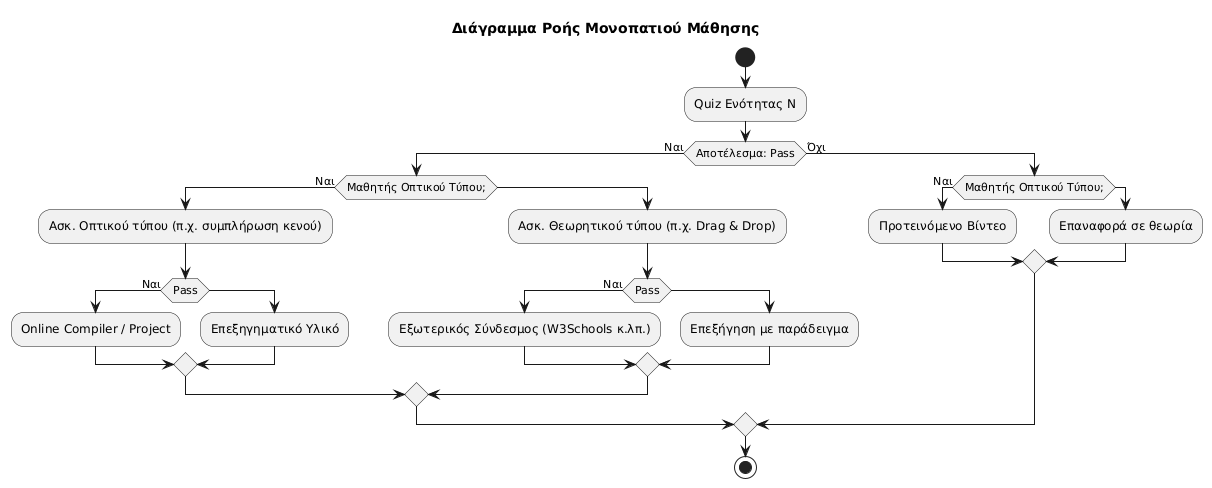
\includegraphics[width=0.9\linewidth]{Figures/image001.png}
    \caption{Διάγραμμα Ροής Μονοπατιού Μάθησης}
    \label{fig:learning-flow}
\end{figure}

\begin{figure}[H]
    \centering
    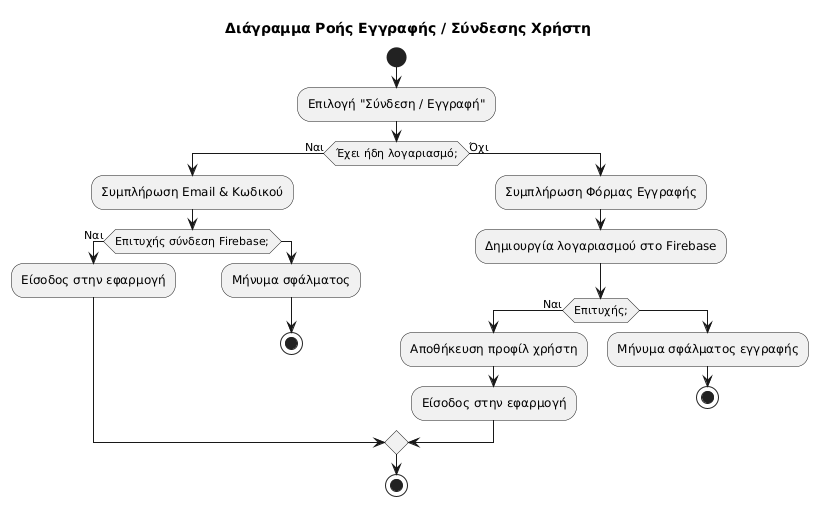
\includegraphics[width=0.9\linewidth]{Figures/image002.png}
    \caption{Διάγραμμα Ροής Εγγραφής / Σύνδεσης Χρήστη}
    \label{fig:signup-flow}
\end{figure}

\begin{figure}[H]
    \centering
    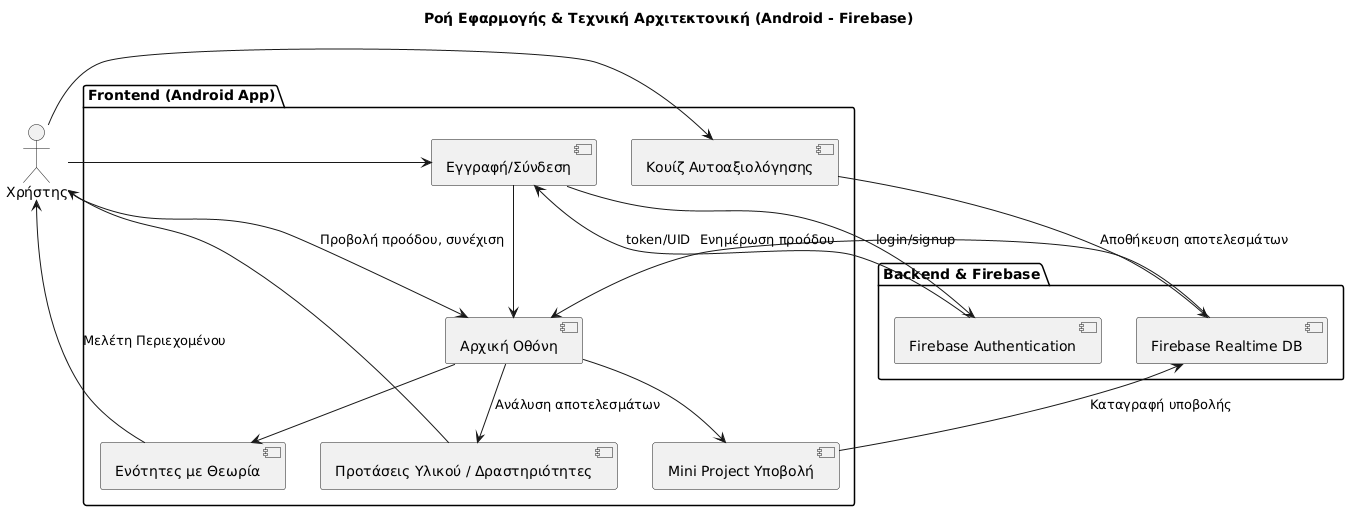
\includegraphics[width=0.9\linewidth]{Figures/image003.png}
    \caption{Ροή Εφαρμογής και Τεχνική Αρχιτεκτονική (Android-Firebase)}
    \label{fig:architecture-flow}
\end{figure}

\begin{figure}[H]
    \centering
    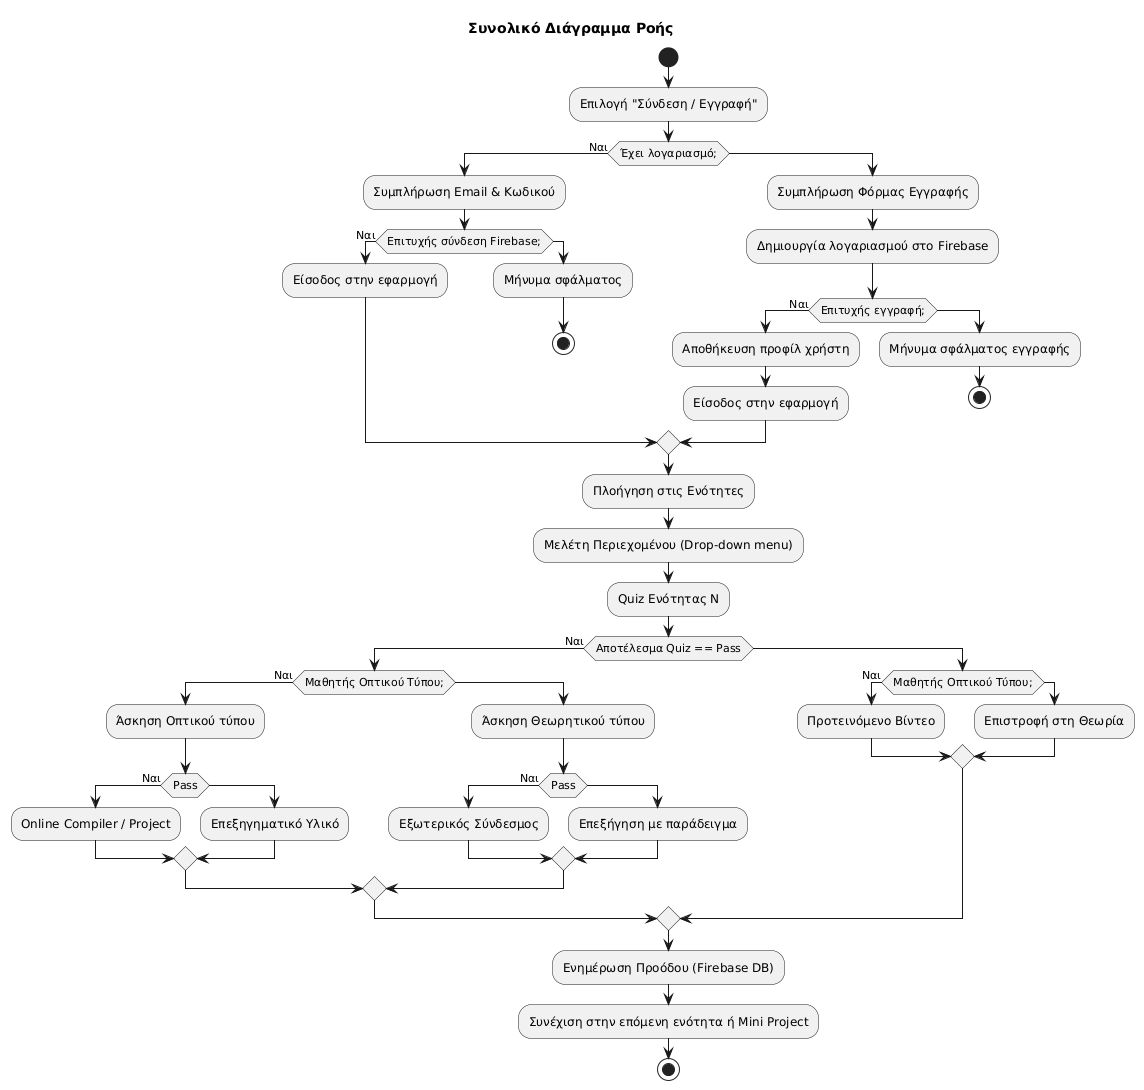
\includegraphics[width=0.9\linewidth]{Figures/image004.png}
    \caption{Συνολικό Διάγραμμα Ροής}
    \label{fig:architecture-flow}
\end{figure}

\section{Τεχνική Αρχιτεκτονική (Frontend – Backend)}

Η τεχνική αρχιτεκτονική της εφαρμογής βασίζεται στο μοντέλο Client–Server και υλοποιείται αποκλειστικά σε περιβάλλον Android, με χρήση της γλώσσας προγραμματισμού Java, της γλώσσας περιγραφής διεπαφής XML και της πλατφόρμας Firebase για τη διαχείριση της αυθεντικοποίησης και των δεδομένων. Η αρχιτεκτονική διακρίνεται σε δύο κύρια επίπεδα: το frontend, που αφορά το ορατό και διαδραστικό τμήμα της εφαρμογής που χρησιμοποιεί ο μαθητής, και το backend, που περιλαμβάνει τις υπηρεσίες αποθήκευσης δεδομένων και ελέγχου ταυτότητας. 

Το frontend είναι υπεύθυνο για τη σχεδίαση της διεπαφής χρήστη (UI), τη διαχείριση της πλοήγησης στις ενότητες και την παρουσίαση του περιεχομένου. Κάθε \textit{activity} της εφαρμογής αντιστοιχεί σε συγκεκριμένη λειτουργικότητα, όπως η είσοδος χρήστη, η μελέτη θεωρίας, η εκτέλεση quiz ή η προβολή στατιστικών προόδου. Η σχεδίαση του UI πραγματοποιείται με χρήση XML, ενώ η επιχειρησιακή λογική γράφεται σε Java, ακολουθώντας αρχές \textit{modular} και \textit{component-based design}.

Το backend βασίζεται στη χρήση δύο βασικών υπηρεσιών της Firebase:

\begin{itemize}
    \item \textbf{Firebase Authentication:} Διαχειρίζεται την εγγραφή και τη σύνδεση των χρηστών με ασφαλή και ελεγχόμενο τρόπο.
    
    \item \textbf{Firebase Realtime Database:} Επιτρέπει την αποθήκευση, ανάκτηση και συγχρονισμό δεδομένων σε πραγματικό χρόνο. Μέσω αυτής της υπηρεσίας καταγράφεται η πρόοδος του μαθητή, η επίδοσή του στα quiz και άλλες κρίσιμες αλληλεπιδράσεις με την εφαρμογή.
\end{itemize}

Η αρχιτεκτονική είναι σχεδιασμένη με γνώμονα τη φορητότητα, τη σταθερότητα και την επεκτασιμότητα. Παρέχει τις βασικές δυνατότητες που απαιτούνται για την απρόσκοπτη μαθησιακή εμπειρία, ενώ ταυτόχρονα διατηρεί τη δομή της εφαρμογής απλή, ευέλικτη και εύκολα επεκτάσιμη σε μελλοντικές ανάγκες.


\chapter{Περιγραφή Τεχνολογιών}
\section{Γλώσσες \& Εργαλεία Ανάπτυξης}

Η εφαρμογή αναπτύχθηκε εξ ολοκλήρου για λειτουργικό σύστημα Android, αξιοποιώντας τεχνολογίες που υποστηρίζουν τη σύγχρονη ανάπτυξη mobile εφαρμογών με υψηλό βαθμό διαδραστικότητας και συνδεσιμότητας με εξωτερικές υπηρεσίες cloud. Ως βασική γλώσσα προγραμματισμού χρησιμοποιήθηκε η Java, η οποία παραμένει μέχρι σήμερα μια από τις κύριες επιλογές για Android development, χάρη στη σταθερότητα, τη συμβατότητα και την πλήρη υποστήριξή της από το Android SDK. 

Παράλληλα, η περιγραφή της διεπαφής χρήστη πραγματοποιήθηκε μέσω της γλώσσας XML, που αποτελεί το πρότυπο για τη διαμόρφωση του layout σε Android εφαρμογές. Η χρήση XML επιτρέπει την ευέλικτη σχεδίαση διεπαφών, τον διαχωρισμό λογικής από την παρουσίαση και τη χρήση επαναχρησιμοποιήσιμων στοιχείων (UI components). 

Για τον σχεδιασμό, την υλοποίηση και τη διαχείριση του έργου χρησιμοποιήθηκε το Android Studio, το επίσημο ολοκληρωμένο περιβάλλον ανάπτυξης (IDE) της Google για Android. Το Android Studio παρέχει εργαλεία debugging, υποστήριξη για emulators, ενσωματωμένο διαχειριστή πακέτων (Gradle) και δυνατότητες για άμεση προεπισκόπηση των UI αρχείων, γεγονός που διευκολύνει σημαντικά την παραγωγική ανάπτυξη και τη σταδιακή δοκιμή της εφαρμογής. 

\section{Frameworks, Βιβλιοθήκες, Περιβάλλον Ανάπτυξης}

Η εφαρμογή αξιοποίησε επιλεγμένες βιβλιοθήκες και υπηρεσίες της Firebase, προκειμένου να καλυφθούν βασικές λειτουργικές απαιτήσεις όπως η αυθεντικοποίηση χρηστών και η αποθήκευση δεδομένων προόδου. Η Firebase Authentication χρησιμοποιήθηκε για την ασφαλή διαχείριση εγγραφής και σύνδεσης χρηστών μέσω email και κωδικού. Η ενσωμάτωσή της έγινε μέσω του επίσημου SDK της Firebase για Android, το οποίο προσφέρει εύκολη υλοποίηση login/logout λειτουργιών και παρακολούθηση της κατάστασης σύνδεσης χρήστη. 

Η Firebase Realtime Database αξιοποιήθηκε για την αποθήκευση και άμεση ανάκτηση δεδομένων σε πραγματικό χρόνο. Η βάση αυτή χρησιμοποιεί JSON ως μορφή δομής δεδομένων και επιτρέπει την ασύγχρονη επικοινωνία με το frontend της εφαρμογής, υποστηρίζοντας real-time updates (π.χ. καταγραφή quiz, στατιστικά, προόδου χρήστη). 

Στο επίπεδο της οπτικοποίησης και της διαδραστικότητας, χρησιμοποιήθηκαν ενσωματωμένα UI components του Android SDK όπως τα RecyclerView, CardView, Buttons, Spinners και Fragments, για την παρουσίαση του περιεχομένου, τη διαχείριση της πλοήγησης και τη δομημένη απεικόνιση των quiz και των επιλογών του χρήστη. 

Το περιβάλλον ανάπτυξης ήταν το Android Studio σε συνδυασμό με τον Android Emulator, για τη δοκιμή της εφαρμογής σε εικονικές συσκευές διαφορετικών διαστάσεων και εκδόσεων Android. Επίσης, έγινε χρήση του Gradle ως εργαλείο διαχείρισης εξαρτήσεων και build automation, εξασφαλίζοντας συνεπή και οργανωμένη διαχείριση του project. 

Τέλος, η διασύνδεση της εφαρμογής με το Firebase πραγματοποιήθηκε μέσω των Google Services JSON configuration files, που διασφαλίζουν σωστό routing και ασφάλεια των credentials κάθε χρήστη στο σύστημα. 

\chapter{Περιγραφή Βάσης Δεδομένων}
\section{Δομή}

Η βάση δεδομένων της εφαρμογής έχει σχεδιαστεί και υλοποιηθεί με τη χρήση του Firebase Realtime Database, μιας πλατφόρμας αποθήκευσης δεδομένων που βασίζεται στο cloud και επιτρέπει τη διαχείριση πληροφοριών σε πραγματικό χρόνο. Η συγκεκριμένη βάση δεν ακολουθεί σχεσιακό μοντέλο (SQL), αλλά χρησιμοποιεί μια ιεραρχική, δενδροειδή δομή τύπου JSON, γεγονός που προσφέρει αυξημένη ευελιξία στην οργάνωση των δεδομένων, εξαιρετική ταχύτητα στην ανάκτηση και ενημέρωσή τους, καθώς και υποστήριξη για ταυτόχρονη συγχρονισμένη πρόσβαση από πολλαπλούς χρήστες. Αυτή η επιλογή κρίθηκε καταλληλότερη για την παρούσα εφαρμογή, η οποία απαιτεί διαρκή ενημέρωση των εκπαιδευτικών δεδομένων, ατομική παρακολούθηση της πορείας του κάθε μαθητή και δυναμική προσαρμογή του περιεχομένου με βάση το μαθησιακό του προφίλ.

Η συνολική αρχιτεκτονική της βάσης διακρίνεται σε δύο θεμελιώδεις κόμβους: τον κόμβο lessons, που περιλαμβάνει το εκπαιδευτικό περιεχόμενο, και τον κόμβο users, όπου αποθηκεύονται όλα τα δεδομένα που σχετίζονται με τον εκάστοτε χρήστη. Η οργάνωση κάθε μαθήματος γίνεται με βάση ένα μοναδικό αναγνωριστικό (π.χ. lesson\_1, lesson\_2 κ.λπ.), κάτω από το οποίο ενσωματώνεται πλήρως το υλικό της αντίστοιχης ενότητας. Η πληροφορία αυτή δομείται με συνέπεια και περιλαμβάνει μεταξύ άλλων τον τίτλο της ενότητας, τη θεωρία διαχωρισμένη σε επιμέρους υποενότητες με τίτλο και περιεχόμενο, τα quiz αξιολόγησης, καθώς και ενισχυτικό υλικό για την περίπτωση επιτυχίας ή αποτυχίας του μαθητή. Το θεωρητικό περιεχόμενο οργανώνεται σε τμήματα τύπου section, με στόχο τη διατήρηση σαφούς και ευανάγνωστης δομής, ώστε να διευκολύνεται τόσο η διδασκαλία όσο και η τεχνολογική διαχείριση της πληροφορίας.

Ιδιαίτερη έμφαση δίνεται στο υποσύστημα των quiz, το οποίο έχει σχεδιαστεί ώστε να μπορεί να φιλοξενήσει διαφορετικού τύπου ερωτήσεις, με σαφή καταγραφή της εκφώνησης, των πιθανών απαντήσεων και της σωστής επιλογής. Τα quiz αποτελούν βασικό εργαλείο αξιολόγησης, ενώ με την ολοκλήρωσή τους ενεργοποιείται και ο μηχανισμός εξατομικευμένης ανατροφοδότησης. Για παράδειγμα, σε περίπτωση αποτυχίας, ο χρήστης λαμβάνει πρόταση για παρακολούθηση εξωτερικού εκπαιδευτικού υλικού (π.χ. βίντεο), ενώ σε περίπτωση επιτυχίας του δίνεται η δυνατότητα να εμβαθύνει περαιτέρω μέσω εμπλουτισμένων θεωρητικών πηγών. Το περιεχόμενο αυτό διαχωρίζεται με σαφήνεια στο πεδίο pass και fail αντίστοιχα.

Από την άλλη πλευρά, ο κόμβος των χρηστών (users) αποτελεί το δεύτερο δομικό πυρήνα της βάσης. Κάθε χρήστης ταυτοποιείται με ένα μοναδικό ID, κάτω από το οποίο αποθηκεύονται όλα τα δεδομένα που αφορούν την ταυτότητά του, την εκπαιδευτική του πορεία, τις επιδόσεις και τον προσωπικό του ρυθμό μάθησης. Αυτή η οργάνωση επιτρέπει στο σύστημα να λειτουργεί όχι μόνο ως εργαλείο καταγραφής, αλλά και ως μηχανισμός ενεργής παρακολούθησης και δυναμικής προσαρμογής της μαθησιακής εμπειρίας.

\begin{figure}[H]
    \centering
    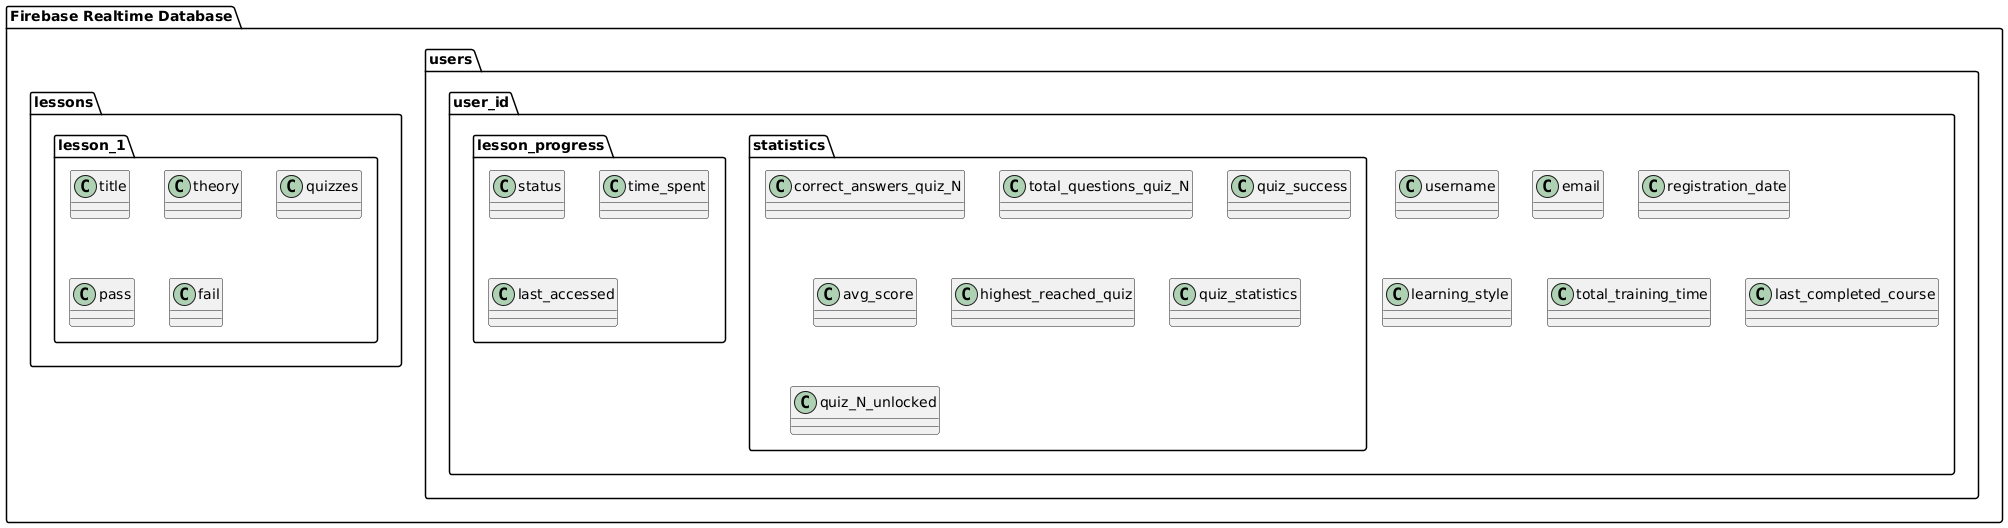
\includegraphics[width=0.9\linewidth]{Figures/image012.png}
    \caption{Απεικόνιση της Βάσης Δεδομένων}
    \label{fig:architecture-flow}
\end{figure}
\section{Πεδία που Καταγράφονται}

Τα δεδομένα που καταγράφονται στη βάση καλύπτουν τόσο την πλευρά του περιεχομένου των μαθημάτων όσο και την πλευρά της χρήσης και της απόδοσης των μαθητών. Από την πλευρά των μαθημάτων (lessons), αποθηκεύονται πληροφορίες που αφορούν τον τίτλο κάθε ενότητας, την οργανωμένη θεωρία σε διακριτά τμήματα, τα quiz αξιολόγησης με πλήρη ανάλυση ανά ερώτηση, καθώς και οι αναφορές στο υποστηρικτικό υλικό που θα προταθεί ανάλογα με το αποτέλεσμα του quiz.

Κάθε θεωρητική ενότητα περιλαμβάνει υποπεδία με τίτλο (title) και περιεχόμενο (content), ενώ τα quiz είναι δομημένα με ερωτήσεις (question), πίνακα απαντήσεων (options) και πεδίο που δηλώνει ποια απάντηση είναι σωστή (is\_correct). Η πληροφορία αυτή είναι επεκτάσιμη και μπορεί να εμπλουτίζεται δυναμικά με νέα ερωτήματα, νέα παραδείγματα ή προσθήκες στο υλικό. Επιπλέον, ανάλογα με την απόδοση του χρήστη, ενεργοποιείται είτε το πεδίο pass, το οποίο οδηγεί σε ενισχυτικό θεωρητικό περιεχόμενο (π.χ. άρθρα), είτε το fail, που παραπέμπει συνήθως σε επεξηγηματικά βίντεο ή επιπλέον ασκήσεις.

Από την πλευρά του χρήστη (users > user\_id), καταγράφονται στοιχεία που επιτρέπουν την πλήρη προσωποποίηση της εμπειρίας και την ακριβή παρακολούθηση της προόδου. Αρχικά, αποθηκεύονται βασικά στοιχεία, όπως το όνομα χρήστη (username), το email (email) και η ημερομηνία εγγραφής (registration\_date). Το μαθησιακό προφίλ (learning\_style) παίζει καθοριστικό ρόλο, καθώς με βάση την επιλογή του (οπτικός ή θεωρητικός μαθητής), προσαρμόζεται το υλικό που προβάλλεται στην εκπαιδευτική πλατφόρμα.

Ιδιαίτερης σημασίας είναι το αντικείμενο lesson\_progress, το οποίο παρακολουθεί για κάθε ενότητα την κατάστασή της (π.χ. αν είναι ενεργή ή έχει ολοκληρωθεί), τον χρόνο που έχει αφιερώσει ο μαθητής σε αυτήν, καθώς και την τελευταία φορά που την επισκέφθηκε. Με αυτό τον τρόπο, η εφαρμογή διαμορφώνει μια συνεχώς ενημερωμένη εικόνα της εμπλοκής του χρήστη με το περιεχόμενο.

Το πιο λεπτομερές και αναλυτικό σύστημα καταγραφής είναι το statistics, το οποίο περιλαμβάνει δεδομένα απόδοσης. Εκεί καταγράφονται ο αριθμός σωστών απαντήσεων σε κάθε quiz (correct\_answers\_quiz\_N), ο συνολικός αριθμός ερωτήσεων (total\_questions\_quiz\_N), το ποσοστό επιτυχίας (avg\_score), η ένδειξη εάν το quiz θεωρείται επιτυχημένο ή όχι (quiz\_success), καθώς και ο δείκτης του πιο πρόσφατα ξεκλειδωμένου quiz (highest\_reached\_quiz). Το ειδικό πεδίο quiz\_statistics προσφέρει μια συγκεντρωτική εικόνα του τελευταίου quiz που ολοκληρώθηκε, με στόχο τη δυναμική προσαρμογή της επόμενης μαθησιακής πρόκλησης.

Τέλος, το πεδίο total\_training\_time καταγράφει συνολικά τον χρόνο που έχει αφιερώσει ο χρήστης στην εφαρμογή, ενώ το last\_completed\_course αποτυπώνει την τελευταία ενότητα που ολοκληρώθηκε επιτυχώς. Η πλήρης αυτή αποτύπωση επιτρέπει την αξιολόγηση της συνέπειας, της προόδου και της γενικότερης ενασχόλησης του μαθητή με το περιβάλλον μάθησης, ενώ λειτουργεί ως βάση για την παροχή προσωποποιημένων συστάσεων και υλικού.

\chapter{Σενάρια Χρήσης}
\section{Ρόλοι Χρηστών}

Η παρούσα εκπαιδευτική εφαρμογή έχει σχεδιαστεί αποκλειστικά με επίκεντρο τον ρόλο του μαθητή, ο οποίος αποτελεί τον μοναδικό τύπο χρήστη. Το σύστημα δεν διακρίνει μεταξύ διαχειριστών, εκπαιδευτών ή άλλων επιπέδων πρόσβασης, γεγονός που ενισχύει την απλότητα του σχεδιασμού και εστιάζει πλήρως στην εκπαιδευτική εμπειρία. Ο μαθητής, ως βασικός φορέας αλληλεπίδρασης με την εφαρμογή, έχει τη δυνατότητα να εγγραφεί και να εισέλθει στο περιβάλλον μάθησης, να περιηγηθεί στις ενότητες, να μελετήσει θεωρία, να συμμετάσχει σε ασκήσεις αξιολόγησης και να παρακολουθήσει την πρόοδό του σε πραγματικό χρόνο. 

Κατά την εγγραφή του, ο μαθητής καταχωρεί βασικά στοιχεία ταυτοποίησης, ενώ ταυτόχρονα του αποδίδεται ένα προφίλ μάθησης, το οποίο μπορεί να οριστεί από τον ίδιο. Το προφίλ αυτό επηρεάζει άμεσα τις ενισχυτικές προτάσεις που λαμβάνει μετά από κάθε δραστηριότητα. Ο ρόλος του μαθητή στην εφαρμογή είναι επομένως διττός: από τη μία πλευρά είναι δέκτης δομημένης γνώσης, ενώ από την άλλη αποτελεί ενεργό παράγοντα στον καθορισμό της πορείας του, λαμβάνοντας αποφάσεις για την πρόοδό του και αναπτύσσοντας αυτορρυθμιστικές δεξιότητες. 

\section{Χρήση Ανά Ενότητα – Περιγραφή Εμπειρίας}

Η εμπειρία χρήσης για τον μαθητή έχει σχεδιαστεί ώστε να είναι σταδιακή, εστιασμένη και παιδαγωγικά οργανωμένη σε ενότητες. Κατά την είσοδό του στην εφαρμογή, ο μαθητής μεταβαίνει στην αρχική οθόνη, όπου του παρουσιάζονται όλες οι ενότητες του εκπαιδευτικού υλικού. Αν και οι ενότητες είναι προσβάσιμες ανά πάσα στιγμή για μελέτη, η πρόοδος στις ασκήσεις και η ενεργοποίηση των κουίζ γίνεται σταδιακά, με βάση την επιτυχή ολοκλήρωση των προηγούμενων αξιολογήσεων. Ο μαθητής μπορεί να επιλέξει οποιαδήποτε ενότητα για να μελετήσει θεωρία, να δει παραδείγματα ή να εξερευνήσει τον τρόπο εφαρμογής βασικών εννοιών. 

Η μελέτη γίνεται μέσω εύχρηστης πλοήγησης τύπου drop-down menu, ενώ η κάθε ενότητα εμπλουτίζεται με διαδραστικά στοιχεία όπως ενδεικτικά παραδείγματα. Μετά τη θεωρητική ενασχόληση, ο μαθητής καλείται να συμμετάσχει στο quiz της ενότητας, το οποίο λειτουργεί ως σημείο ελέγχου κατανόησης. Ανάλογα με την απόδοσή του στο quiz, η εφαρμογή του προτείνει ενισχυτικό υλικό: αυτό μπορεί να είναι οπτικής φύσης, όπως βίντεο, ή θεωρητικό, όπως επεξηγηματικά κείμενα. Η πρόταση είναι εξατομικευμένη και βασίζεται στο μαθησιακό προφίλ του χρήστη. 

Καθώς ο μαθητής προχωρά μέσα από τις ενότητες, το επίπεδο δυσκολίας αυξάνεται σταδιακά. Η τελική ενότητα περιλαμβάνει ένα mini project, στο οποίο ο μαθητής καλείται να εφαρμόσει όσα έχει μάθει, σχεδιάζοντας και υλοποιώντας μια μικρή προγραμματιστική εργασία. Η διαδικασία αυτή ενισχύει την αίσθηση ολοκλήρωσης, παρέχει κίνητρο και επιβραβεύει τη συστηματική προσπάθεια.  


\chapter{Μηχανισμοί Προσαρμοσμένης Μάθησης (Adaptive Learning)}
\section{Τρόποι Δυναμικής Προσαρμογής Περιεχομένου}

Η εφαρμογή αξιοποιεί τεχνικές δυναμικής προσαρμογής περιεχομένου, οι οποίες βασίζονται στην επίδοση του χρήστη, στο μαθησιακό του προφίλ και στη συμπεριφορά του κατά την πλοήγηση. Σε κάθε ενότητα, ο μαθητής μελετά το θεωρητικό υλικό και καλείται να απαντήσει σε ένα σύνολο ερωτήσεων τύπου quiz. Ανάλογα με το αποτέλεσμα (pass/fail), ενεργοποιούνται διαφορετικές διαδρομές μάθησης. Επιπλέον, οι επιλογές προσαρμόζονται στο στυλ μάθησης του χρήστη, το οποίο έχει καθοριστεί κατά την εγγραφή. 

Σε περίπτωση αποτυχίας, η εφαρμογή επιλέγει ανάμεσα σε υποστηρικτικό οπτικό υλικό (όπως βίντεο) ή θεωρητικό υλικό (επαναφορά στη θεωρία) για να βοηθήσει τον μαθητή να αναστοχαστεί πάνω στο περιεχόμενο. Αντίθετα, όταν ο μαθητής επιτύχει στο quiz, το σύστημα τον ενθαρρύνει να συμμετάσχει σε προαιρετικές ενισχυτικές δραστηριότητες υψηλότερης δυσκολίας ή πιο δημιουργικής φύσης, όπως συμπλήρωση κενών, drag and drop, προβλήματα ανάλυσης ή σύνδεση με εξωτερικές πλατφόρμες όπως το W3Schools και το CodeCombat. 

Η προσαρμογή γίνεται σε πραγματικό χρόνο και εξαρτάται από την τρέχουσα απόδοση, τον αριθμό προσπαθειών, τη χρονική διάρκεια μελέτης και την ιστορική πορεία του χρήστη. Έτσι, το περιεχόμενο "ξεδιπλώνεται" σταδιακά, εστιάζοντας στην ενίσχυση των αδυναμιών και την καλλιέργεια αυτοπεποίθησης. 

\section{Λογική Εξατομίκευσης και Επιλογής Υλικού}

Ο μηχανισμός εξατομίκευσης στην εφαρμογή δεν βασίζεται σε μια στατική προκαθορισμένη ροή μάθησης, αλλά σε μια δυναμική και ευέλικτη λογική που λαμβάνει υπόψη δύο βασικές παραμέτρους: το μαθησιακό προφίλ του χρήστη και την αποδοτικότητά του στις αξιολογήσεις. 

Ο πρώτος και θεμελιώδης άξονας είναι το μαθησιακό στυλ. Κατά την εγγραφή, κάθε μαθητής εντοπίζεται οπτικός ή θεωρητικός τύπος. Αυτή η κατηγοριοποίηση δεν επηρεάζει μόνο το περιεχόμενο που του προτείνεται σε περιπτώσεις αποτυχίας, αλλά επεκτείνεται και στον τύπο ενισχυτικών δραστηριοτήτων μετά από επιτυχή απόδοση. Για παράδειγμα, ένας οπτικός μαθητής που αποτυγχάνει στο quiz οδηγείται σε υποστηρικτικό βίντεο, ενώ ένας θεωρητικός μαθητής οδηγείται σε επανεξέταση θεωρίας. Αντίστοιχα, ένας επιτυχημένος θεωρητικός χρήστης μπορεί να οδηγηθεί σε λογικές ασκήσεις τύπου Drag and Drop με κριτική σκέψη, ενώ ένας επιτυχημένος οπτικός σε διαδραστικές ασκήσεις συμπλήρωσης κενού ή προγραμματισμό μέσα σε γραφικό compiler. 

Ο δεύτερος άξονας αφορά την επίδοση. Η εφαρμογή δεν αξιολογεί μόνο το τελικό αποτέλεσμα ενός quiz, αλλά και παραμέτρους όπως η συνολική ακρίβεια, η ταχύτητα ολοκλήρωσης, ο αριθμός προσπαθειών, καθώς και το είδος των λαθών. Για παράδειγμα, ένας μαθητής που αποτυγχάνει σε ερωτήσεις κατανόησης εννοιών οδηγείται σε θεωρία, ενώ κάποιος που αποτυγχάνει σε εφαρμοστικά σενάρια προτρέπεται να εξερευνήσει εξωτερικές πλατφόρμες, όπως το W3Schools για εμβάθυνση ή το CodeCombat για προγραμματιστική εξάσκηση μέσα από παιχνιδοποιημένο περιβάλλον. 

Η λογική επιλογής υλικού δεν είναι γραμμική ούτε τυχαία, αλλά βασίζεται σε πραγματικά δεδομένα και συνδυαστική ανάλυση. Αυτό επιτρέπει στην εφαρμογή να καθοδηγεί τον μαθητή χωρίς να τον περιορίζει, να του προσφέρει εναλλακτικές, αλλά και να εξασφαλίζει ότι κάθε του βήμα είναι παιδαγωγικά τεκμηριωμένο και λειτουργικά στοχευμένο.

\section{Μονοπάτια Μάθησης Ανά Ενότητα}

Κάθε διδακτική ενότητα της εφαρμογής αποτελεί έναν μικρό κύκλο μάθησης, στον οποίο ο χρήστης ακολουθεί διαφορετικά μονοπάτια, ανάλογα με τις επιδόσεις και τις ανάγκες του. Το σύστημα έχει υλοποιηθεί έτσι ώστε η ροή μάθησης να είναι μη-γραμμική, αποκλίνουσα και προσαρμόσιμη, διασφαλίζοντας μια εμπειρία μάθησης που δεν ακολουθεί το ίδιο μοτίβο για όλους. 

\begin{figure}[H]
    \centering
    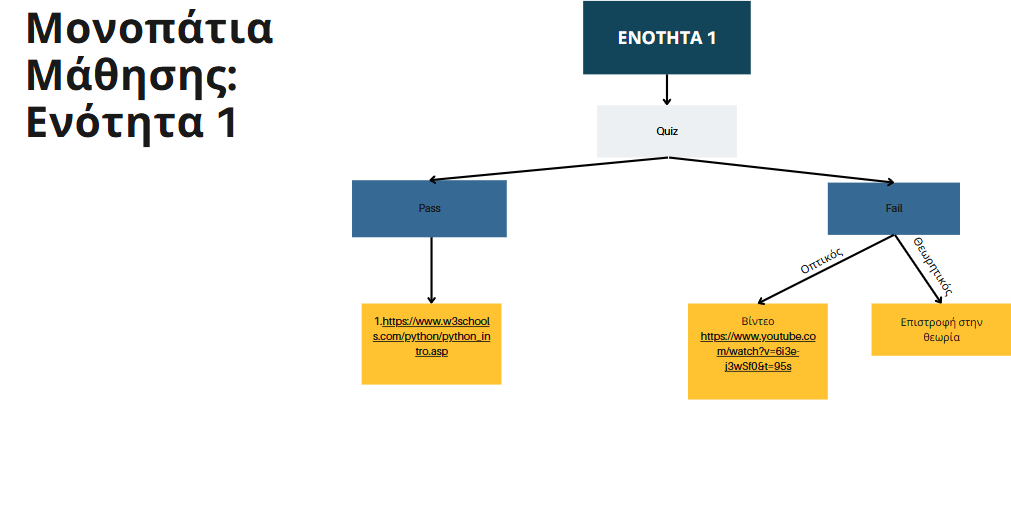
\includegraphics[width=0.9\linewidth]{Figures/image006.png}
    \caption{Ενότητα 1}
    \label{fig:enter-label}
\end{figure}

Στην Ενότητα 1, το μονοπάτι μάθησης είναι εισαγωγικό και προσαρμοσμένο ώστε να κατευθύνει τον μαθητή ομαλά στην πρώτη επαφή με την εκπαιδευτική διαδικασία. Μετά τη μελέτη της θεωρίας, ο μαθητής καλείται να απαντήσει στο quiz αξιολόγησης. Αν το αποτέλεσμα είναι επιτυχές, του προτείνεται η εθελοντική εμβάθυνση στην ενότητα μέσω του W3Schools Python Intro, ως μία πρώτη επαφή με εξωτερικές επαγγελματικές πηγές γνώσης. Σε περίπτωση αποτυχίας, ενεργοποιείται ένας μηχανισμός προσαρμογής ανάλογα με τον τύπο μάθησης: οι οπτικοί μαθητές παραπέμπονται σε υποστηρικτικό βίντεο εξήγησης, ενώ οι θεωρητικοί επιστρέφουν σε επανάληψη της βασικής θεωρίας. 

\begin{figure}[H]
    \centering
    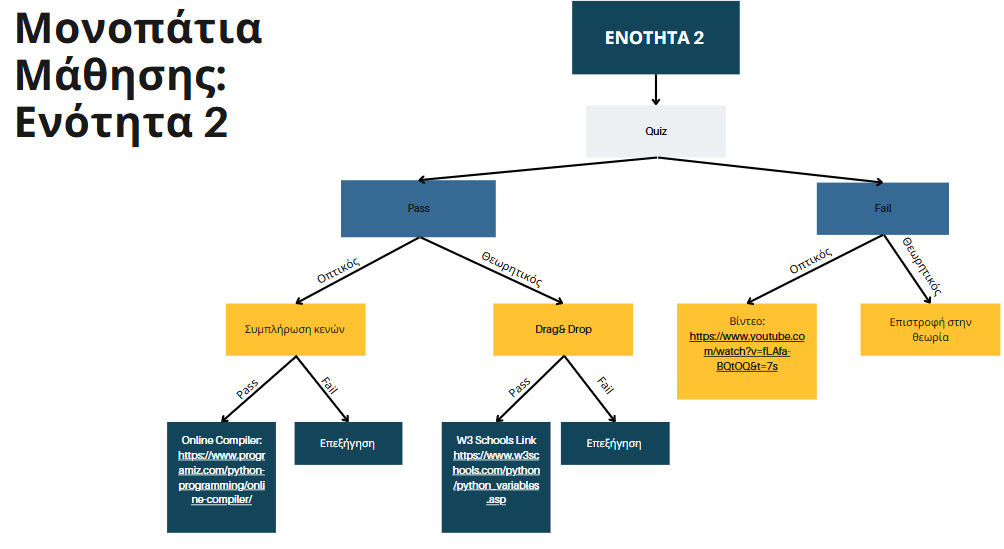
\includegraphics[width=0.9\linewidth]{Figures/image007.png}
    \caption{Ενότητα 2}
    \label{fig:enter-label}
\end{figure}

Η Ενότητα 2 εισάγει τον διαχωρισμό μεταξύ οπτικού και θεωρητικού τύπου μάθησης μετά από επιτυχή ολοκλήρωση του quiz. Οι οπτικοί προχωρούν σε άσκηση συμπλήρωσης κενών και, εφόσον την ολοκληρώσουν επιτυχώς, οδηγούνται στον Online Compiler της Programiz για πρακτική εφαρμογή. Σε περίπτωση αποτυχίας, εμφανίζεται ενισχυτικό παράδειγμα και εξήγηση. Αντίστοιχα, οι θεωρητικοί χρήστες εκτελούν άσκηση τύπου Drag and Drop και, εφόσον επιτύχουν, οδηγούνται σε παραπομπή για επεξήγηση μεταβλητών στον W3Schools Variables, ενώ στην αποτυχία λαμβάνουν διδακτικό feedback. Σε κάθε αποτυχία στο quiz της ενότητας, η διαδικασία επαναλαμβάνεται όπως και στην πρώτη, με προσαρμογή υλικού ανάλογα με το μαθησιακό προφίλ. 

\begin{figure}[H]
    \centering
    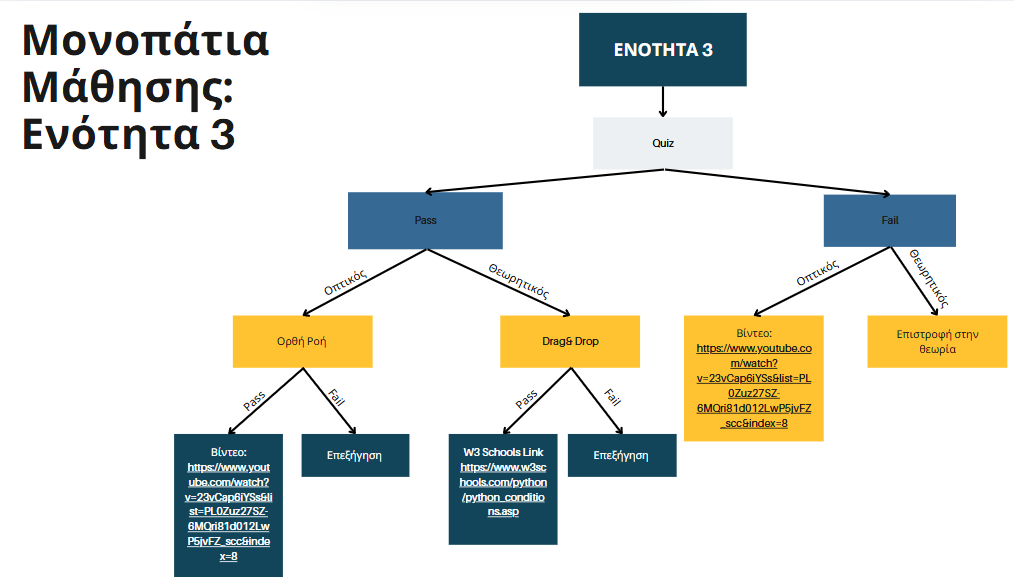
\includegraphics[width=0.9\linewidth]{Figures/image008.png}
    \caption{Ενότητα 3}
    \label{fig:enter-label}
\end{figure}

Η Ενότητα 3 διαφοροποιείται σημαντικά ως προς τη φύση των ασκήσεων μετά το quiz. Στην επιτυχή ολοκλήρωση, οι οπτικοί χρήστες οδηγούνται σε άσκηση σωστής ροής, η οποία ενισχύεται με βίντεο παραδειγμάτων αν περάσουν, ή σε επεξήγηση αν αποτύχουν. Αντίστοιχα, οι θεωρητικοί χρήστες εργάζονται με νέα άσκηση Drag and Drop, με εναλλακτική προώθηση προς το W3Schools Conditions ή εκπαιδευτική υποστήριξη. Σε αποτυχία στο quiz, η ροή επαναλαμβάνεται με επιστροφή σε θεωρία για θεωρητικούς, και διδακτικό βίντεο για τους οπτικούς. 

\begin{figure}[H]
    \centering
    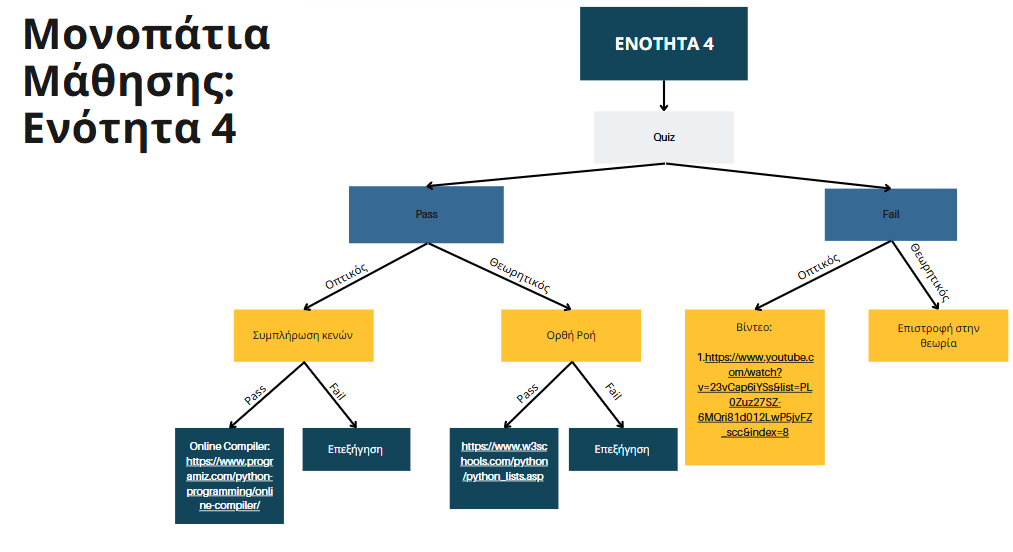
\includegraphics[width=0.9\linewidth]{Figures/image009.png}
    \caption{Ενότητα 4}
    \label{fig:enter-label}
\end{figure}

Η Ενότητα 4 ανεβάζει τον βαθμό δυσκολίας και περιλαμβάνει δύο εναλλακτικές κατευθύνσεις μετά την επιτυχία. Οι οπτικοί μαθητές καλούνται να λύσουν συμπλήρωση κενών με αυξημένη δυσκολία και, αν πετύχουν, συνεχίζουν σε εφαρμογή μέσω του Online Compiler. Οι θεωρητικοί αντιμετωπίζουν άσκηση “Ορθή Ροή” (λογική αλληλουχία βημάτων), η οποία, αν αποδώσει θετικά, οδηγεί σε ένα κομμάτι της θεωρίας στο W3Schools. Σε αποτυχία, παρέχεται ενίσχυση. Σε περίπτωση αποτυχίας στο quiz, προτείνεται σειρά βίντεο εξηγήσεων για οπτικούς ή επιστροφή στη θεωρία για θεωρητικούς. 

\begin{figure}[H]
    \centering
    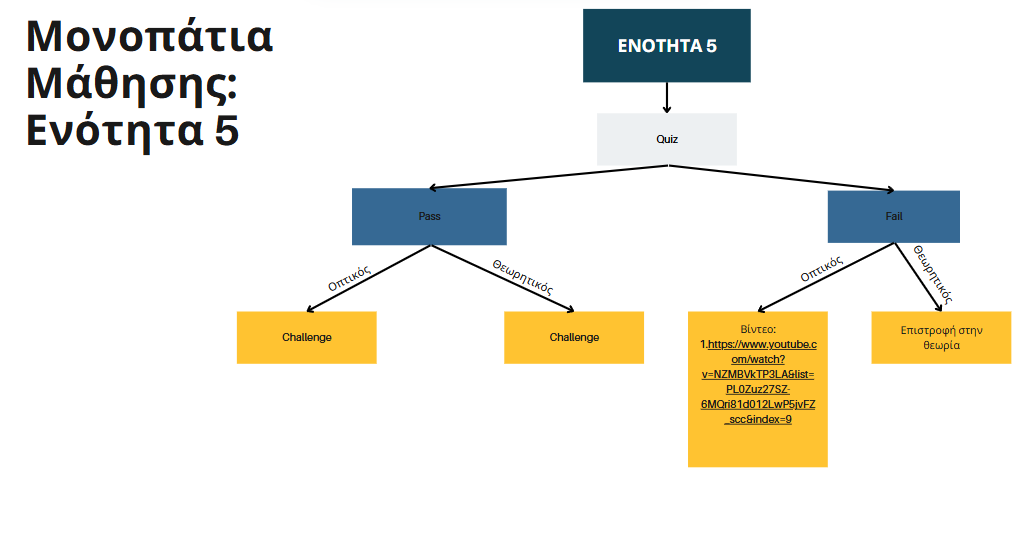
\includegraphics[width=0.9\linewidth]{Figures/image010.png}
    \caption{Ενότητα 5}
    \label{fig:enter-label}
\end{figure}

Στην Ενότητα 5, η μαθησιακή πορεία αποκτά πιο σύνθετο και δημιουργικό χαρακτήρα. Μετά την ολοκλήρωση του quiz, οι χρήστες που πετυχαίνουν διαχωρίζονται ξανά ανάλογα με το μαθησιακό τους προφίλ. Τόσο οι οπτικοί όσο και οι θεωρητικοί χρήστες καλούνται να εκτελέσουν ένα challenge δραστηριότητας. Ο στόχος σε αυτή τη φάση είναι η ενίσχυση της αυτενέργειας και η εξάσκηση σε σενάρια που απαιτούν συνδυασμό γνώσεων. Αντίθετα, οι μαθητές που αποτυγχάνουν στο quiz της ενότητας οδηγούνται είτε σε βίντεο ενίσχυσης με χρήση συναρτήσεων, είτε σε επιστροφή στο θεωρητικό υλικό, ανάλογα με τον τύπο μάθησης τους. Αυτή η δομή κλιμακώνει τη δυσκολία και προετοιμάζει τον μαθητή για την τελική αξιολόγηση και το project. 

\begin{figure}[H]
    \centering
    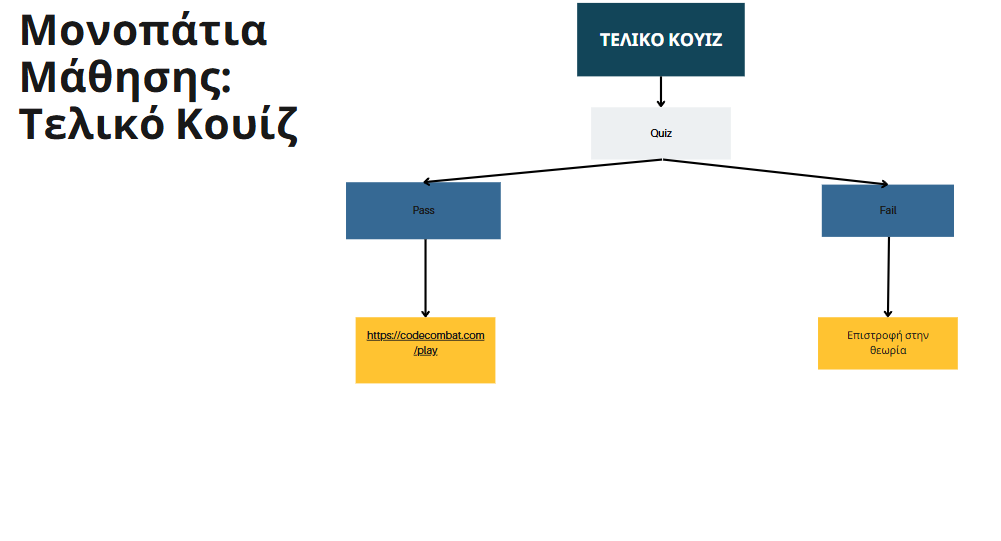
\includegraphics[width=0.9\linewidth]{Figures/image011.png}
    \caption{Τελικό Κουιζ}
    \label{fig:enter-label}
\end{figure}

Τέλος, στο Τελικό Quiz, η αξιολόγηση λειτουργεί ως αποκορύφωμα της μαθησιακής διαδικασίας. Οι μαθητές καλούνται να απαντήσουν σε ερωτήσεις που συνοψίζουν και συνθέτουν όσα έχουν μάθει στις πέντε προηγούμενες ενότητες. Σε περίπτωση επιτυχίας, οι χρήστες μεταφέρονται στο CodeCombat, ένα διαδραστικό, παιχνιδοποιημένο περιβάλλον προγραμματισμού, το οποίο λειτουργεί ως πλατφόρμα εφαρμογής της γνώσης μέσα από προκλήσεις. Η εμπειρία αυτή εξυπηρετεί τη μετατροπή της παθητικής γνώσης σε ενεργή δράση, ενισχύοντας την κριτική σκέψη και την επιδεξιότητα επίλυσης προβλημάτων. Αντίθετα, όσοι αποτυγχάνουν επιστρέφουν στη θεωρία για στοχευμένη επανεξάσκηση, ώστε να εξασφαλιστεί η επάρκεια πριν την οριστική ολοκλήρωση. 

Κάθε μονοπάτι στις παραπάνω ενότητες δεν είναι απλώς διαδρομή πρόοδου, αλλά παιδαγωγικά τεκμηριωμένο σχήμα προσαρμογής που συνδυάζει απόδοση, στυλ μάθησης και προτεινόμενα περιβάλλοντα εμβάθυνσης. Οι εξωτερικοί σύνδεσμοι, τα είδη των ασκήσεων και η δυναμική μεταπήδηση σε νέο περιεχόμενο συγκροτούν ένα συνεκτικό σύστημα εξατομικευμένης μάθησης που προετοιμάζει τον μαθητή για το τελικό στάδιο αξιολόγησης και δημιουργικής εφαρμογής. 

\chapter{Διαχείριση Στατιστικών και Προόδου}
\section{Τι Αποθηκεύεται – Πώς Αξιοποιείται}

Η εκπαιδευτική εφαρμογή καταγράφει και αποθηκεύει σε πραγματικό χρόνο ένα οργανωμένο σύνολο στατιστικών δεδομένων που σχετίζονται με την απόδοση, την πρόοδο και τη μαθησιακή πορεία κάθε χρήστη.Τα δεδομένα αυτά δεν συλλέγονται απλώς για αρχειοθέτηση, αλλά αξιοποιούνται ενεργά για την προσαρμογή της εμπειρίας χρήσης, την υποστήριξη της εξατομίκευσης και τη συνολική ενίσχυση της εκπαιδευτικής διαδικασίας.Η αποθήκευση πραγματοποιείται στο περιβάλλον \textit{Firebase Realtime Database}, με δομή \texttt{JSON}. Κάθε χρήστης αναγνωρίζεται μέσω μοναδικού αναγνωριστικού (\texttt{UID}), και τα δεδομένα οργανώνονται σε προσωπικό κόμβο.

\vspace{1em}
Για κάθε χρήστη καταγράφονται:

\begin{itemize}
    \item Η συνολική διάρκεια ενασχόλησης με την εφαρμογή (\texttt{total\_training\_time}), που απεικονίζει τον συνολικό χρόνο μελέτης.
    \item Η πρόοδος σε σχέση με τα quiz, με πεδία που δείχνουν τον αριθμό του πιο πρόσφατα ξεκλειδωμένου quiz (\texttt{highest\_reached\_quiz}).
    \item Η μαθησιακή προτίμηση (\texttt{learning\_style}), που επιδρά στον τύπο της ανατροφοδότησης (π.χ. θεωρητικό ή οπτικό υλικό).
    \item Τα αποτελέσματα των quiz: αριθμός σωστών και λανθασμένων απαντήσεων ανά quiz, ο συνολικός αριθμός ερωτήσεων, καθώς και αν ο χρήστης πέτυχε το ελάχιστο ποσοστό επιτυχίας (\texttt{quiz\_success}).
    \item Το μέσο ποσοστό επιτυχίας (\texttt{avg\_score}), που υπολογίζεται με βάση τα quiz που έχουν απαντηθεί.
    \item Η ολοκλήρωση δραστηριοτήτων ή mini projects, με αντίστοιχα \texttt{flags} ή δείκτες στη βάση δεδομένων.
\end{itemize}

\vspace{1em}
Τα δεδομένα αυτά χρησιμοποιούνται για:

\begin{itemize}
    \item Την προσαρμογή της εκπαιδευτικής ροής: επιτυχίες οδηγούν σε νέα υλικά και δραστηριότητες, ενώ αποτυχίες ενεργοποιούν υποστηρικτικό περιεχόμενο.
    \item Την προβολή κατάλληλων ειδοποιήσεων ή βίντεο, με βάση τον τύπο μάθησης.
    \item Τη συνολική διαχείριση της εμπειρίας χρήσης, εξασφαλίζοντας ότι κάθε μαθητής προχωρά με το δικό του ρυθμό και τις δικές του ανάγκες.
\end{itemize}
  

\section{Παρουσίαση μέσω Analytics}

Η παρουσίαση των παραπάνω δεδομένων στον ίδιο τον μαθητή γίνεται με φιλικό, διαδραστικό και κατανοητό τρόπο. Η εφαρμογή εμφανίζει έναν πίνακα προόδου με τα τρέχοντα στατστικά του προφίλ του.

Προβάλλονται στατιστικά στοιχεία για τον συνολικό χρόνο μελέτης, του τελευταίου κουιζ που έγινε, τη συχνότητα ενασχόλησης με την εφαρμογή και τη μέση απόδοση, ώστε ο μαθητής να έχει πλήρη εικόνα της πορείας του. Όλα τα δεδομένα ενημερώνονται αυτόματα και παρουσιάζονται μέσω ενός responsive, mobile-friendly περιβάλλοντος, χωρίς να απαιτείται τεχνική κατάρτιση.

Η λειτουργικότητα αυτή ενισχύει την μεταγνωστική επίγνωση του μαθητή — δηλαδή την ικανότητά του να αναγνωρίζει τι έχει μάθει και τι πρέπει να βελτιώσει. Παράλληλα, υποστηρίζει τη διαδικασία της αυτορρυθμιζόμενης μάθησης, δίνοντάς του τη δυνατότητα να αποφασίζει πότε χρειάζεται επανάληψη, πότε να προχωρήσει, ή πότε να επιστρέψει σε προγενέστερη ενότητα. Η συνολική διαχείριση των στατιστικών, τόσο σε επίπεδο backend όσο και στον τρόπο προβολής τους, συνιστά έναν από τους πυλώνες της παιδαγωγικής αποτελεσματικότητας της εφαρμογής. 
\chapter{Περιγραφή Κώδικα}

\section{Περιγραφή Κώδικα και Διασύνδεσης}
\subsection{AdaptiveLearning}

Η κλάση AdaptiveLearning αποτελεί τον πυρήνα της λογικής μιας διαδραστικής, προσαρμοστικής εκπαιδευτικής εφαρμογής για Android, με στόχο την εξατομίκευση της μαθησιακής εμπειρίας βάσει του προφίλ και της επίδοσης του κάθε χρήστη. Μέσω της σύνδεσής της με την υπηρεσία Firebase Realtime Database, η κλάση ανακτά δυναμικά δεδομένα που αφορούν εκπαιδευτικές δραστηριότητες, περιεχόμενο θεωρίας, οδηγίες, σωστές απαντήσεις και στοιχεία αξιολόγησης, και τα αξιοποιεί για να καθορίσει ποια ενότητα και δραστηριότητα είναι καταλληλότερη για κάθε μαθητή. 

Αναγνωρίζοντας το μαθησιακό στυλ του χρήστη (οπτικός ή θεωρητικός) και το αν έχει επιτύχει ή αποτύχει σε σχετικές αξιολογήσεις, η AdaptiveLearning καθοδηγεί την πορεία μάθησης με τρόπο ευέλικτο και προσωποποιημένο. Ανάλογα με την περίπτωση, μπορεί να προτείνει διαδραστικές ασκήσεις τύπου "επιλογής εικόνας", "συμπλήρωσης κενού", "drag and drop" ή "πρόκλησης", να εμφανίσει θεωρητικό υλικό ή να ανακατευθύνει τον χρήστη σε υποστηρικτικό οπτικό περιεχόμενο, όπως βίντεο στο YouTube. Παράλληλα, φροντίζει για την ορθή εκκίνηση των κατάλληλων δραστηριοτήτων μέσα από τις αντίστοιχες Activity κλάσεις του Android και διαχειρίζεται αποτελεσματικά την επικοινωνία με τη βάση, ενσωματώνοντας μηχανισμούς αντιμετώπισης σφαλμάτων. 

\vspace{0.3cm}
\textbf{SelectTheImage} \\

Η μέθοδος SelectTheImage αποτελεί βασικό τμήμα της λογικής μιας διαδραστικής εκπαιδευτικής εφαρμογής που στηρίζεται στην Firebase Realtime Database. Ο ρόλος της είναι να ανακτήσει συγκεκριμένα δεδομένα από τη βάση και να ξεκινήσει τη δραστηριότητα ALSelectTheImageActivity, μέσω της οποίας παρουσιάζεται στον χρήστη μια άσκηση τύπου "επιλογή εικόνας". Η μέθοδος αυτή δέχεται ως παραμέτρους το αναγνωριστικό του μαθήματος, την ενότητα, τον τύπο της δραστηριότητας (οπτικός, θεωρητικός κ.λπ.), καθώς και το context του Android, το οποίο είναι απαραίτητο για την εκκίνηση μιας νέας δραστηριότητας.  

Αρχικά, δημιουργείται μια βασική αναφορά προς το κατάλληλο σημείο της βάσης, που αντιστοιχεί στη διαδρομή lessons/lesson/pass/type. Από εκεί ορίζονται δύο επιμέρους αναφορές: η μία για το exercises, που περιέχει τα δεδομένα της δραστηριότητας, και η άλλη για το url, που περιλαμβάνει το σχετικό εξωτερικό περιεχόμενο, όπως εικόνες ή άλλα μέσα. Η διαδικασία ανάκτησης των δεδομένων πραγματοποιείται βήμα προς βήμα, με χρήση ακροατών (ValueEventListener), οι οποίοι εξασφαλίζουν ότι η εφαρμογή θα συνεχίσει μόνον όταν τα δεδομένα είναι διαθέσιμα.  

Πρώτο βήμα είναι η ανάγνωση του URL από τη βάση. Εφόσον αυτό ληφθεί επιτυχώς, προχωρά η ανάγνωση των blocks του προγράμματος, τα οποία βρίσκονται στον κόμβο exercises/program. Τα blocks αυτά μπορεί να είναι εικόνες, αποσπάσματα κώδικα ή άλλου είδους επιλογές που θα παρουσιαστούν στον χρήστη. Αποθηκεύονται σε λίστα για μεταγενέστερη χρήση. Στη συνέχεια, ανακτώνται οι οδηγίες της άσκησης από τον κόμβο exercises/instruction, ώστε να καταστεί σαφές στον χρήστη τι πρέπει να κάνει. Τελευταίο βήμα στη συλλογή των δεδομένων είναι η ανάκτηση της σωστής απάντησης από τον κόμβο exercises/answers, η οποία θα χρησιμοποιηθεί για την αξιολόγηση της επιλογής του χρήστη.  

Όταν όλα τα παραπάνω δεδομένα έχουν συγκεντρωθεί επιτυχώς, η μέθοδος δημιουργεί ένα Intent για να ξεκινήσει τη δραστηριότητα ALSelectTheImageActivity. Στο Intent περνούν όλα τα απαραίτητα δεδομένα: η λίστα με τα blocks, οι οδηγίες, ο τίτλος της ενότητας, το URL του συνοδευτικού περιεχομένου και η σωστή απάντηση. Η δραστηριότητα ξεκινά με την εντολή context.startActivity(intent), ενεργοποιώντας έτσι τη διεπαφή χρήστη που θα φιλοξενήσει την άσκηση.  

Σε κάθε στάδιο ανάγνωσης από τη βάση, υπάρχει πρόβλεψη για το ενδεχόμενο αποτυχίας σύνδεσης ή πρόσβασης στα δεδομένα. Σε τέτοια περίπτωση, ενεργοποιείται η μέθοδος onCancelled, η οποία εμφανίζει στον χρήστη κατάλληλο μήνυμα σφάλματος μέσω Toast, διασφαλίζοντας ότι υπάρχει πάντα ανάδραση σε προβλήματα και αποτρέποντας την εφαρμογή από το να καταρρεύσει αθόρυβα.  

\vspace{0.3cm}
\textbf{Challenge} \\

Η μέθοδος Challenge είναι υπεύθυνη για την ανάκτηση δεδομένων μιας δραστηριότητας πρόκλησης από τη βάση δεδομένων Firebase και την εκκίνηση της δραστηριότητας ALChallengeActivity για την εμφάνισή της στον χρήστη. Πιο συγκεκριμένα, με βάση τα στοιχεία lesson, unit και type, εντοπίζει τη σωστή διαδρομή στη βάση και αντλεί τρία βασικά δεδομένα: το URL σχετικού περιεχομένου (π.χ. μια εικόνα ή σελίδα), τις οδηγίες της δραστηριότητας και την ενδεικτική λύση (απάντηση). Αφού ανακτηθούν όλα επιτυχώς, δημιουργεί ένα Intent, μεταφέρει τα δεδομένα στην επόμενη δραστηριότητα και την εκκινεί, επιτρέποντας στον χρήστη να δει την πρόκληση με τις οδηγίες, το περιεχόμενο και τη λύση. Πρόκειται για λειτουργικό τμήμα μιας εκπαιδευτικής εφαρμογής που διευκολύνει την εμφάνιση διαδραστικών ασκήσεων βασισμένων σε δεδομένα από τη βάση.  

\vspace{0.3cm}
\textbf{FillTheGaps} \\

Η μέθοδος FillTheGaps ανακτά δεδομένα μιας δραστηριότητας τύπου "Συμπλήρωση κενού" και ξεκινά την αντίστοιχη δραστηριότητα προβολής (ALFillTheBlocksActivity). Συγκεκριμένα, με βάση το μάθημα, την ενότητα και τον τύπο άσκησης, εντοπίζει το κατάλληλο σημείο στη βάση και συλλέγει τα εξής στοιχεία: έναν σύνδεσμο σε σχετικό βίντεο ή περιεχόμενο (url), το πρόγραμμα με κενά που πρέπει να συμπληρωθούν, τις οδηγίες της άσκησης, και μια λίστα με τις σωστές απαντήσεις. Αφού ολοκληρωθεί η συλλογή αυτών των στοιχείων, δημιουργεί ένα Intent, τα επισυνάπτει ως δεδομένα, και εκκινεί τη δραστηριότητα, ώστε ο χρήστης να δει και να αλληλεπιδράσει με την άσκηση. Η μέθοδος περιλαμβάνει επίσης χειρισμό σφαλμάτων για κάθε πιθανό σημείο αποτυχίας ανάκτησης των δεδομένων. 

\vspace{0.3cm}
\textbf{DragAndDrop} \\

Η μέθοδος DragAndDrop αναλαμβάνει να ανακτήσει από τη Firebase δεδομένα μιας διαδραστικής άσκησης τύπου "drag and drop" και να ξεκινήσει την κατάλληλη δραστηριότητα προβολής (ALDragAndDropActivity). Συγκεκριμένα, χρησιμοποιώντας τα ορίσματα lesson, unit και type, εντοπίζει στη βάση το σχετικό περιεχόμενο και αντλεί τέσσερα βασικά στοιχεία: το URL ενός σχετικού βίντεο ή περιεχομένου, το πρόγραμμα προς αναδιάταξη (ως κείμενο), τις οδηγίες της άσκησης, και τις σωστές γραμμές-απαντήσεις. Οι γραμμές αυτές εξάγονται από το πρόγραμμα με διαχωρισμό σε /n, αποθηκεύονται σε λίστα και ελέγχονται για εγκυρότητα. Τέλος, όλα τα δεδομένα προστίθενται σε Intent και η δραστηριότητα εκκινεί, παρουσιάζοντας στον χρήστη την άσκηση. Σε περίπτωση αποτυχίας σε οποιοδήποτε βήμα ανάκτησης, εμφανίζεται σχετικό μήνυμα σφάλματος. Η μέθοδος υποστηρίζει πλήρως τη λειτουργικότητα προβολής μιας drag-and-drop άσκησης βασισμένης σε δυναμικά δεδομένα από τη βάση.  

\vspace{0.3cm}
\textbf{VisualFail} \\

Η μέθοδος VisualFail είναι υπεύθυνη για την εμφάνιση ενός επεξηγηματικού ή υποστηρικτικού βίντεο (συνήθως μετά από αποτυχία σε κάποια δραστηριότητα), το οποίο έχει αποθηκευτεί στη Firebase. Συγκεκριμένα, εντοπίζει το URL του βίντεο στην τοποθεσία lessons/<lesson>/fail/url και, αν το URL είναι έγκυρο, προσπαθεί να το ανοίξει μέσω της εφαρμογής YouTube. Αν η εφαρμογή YouTube δεν είναι εγκατεστημένη στη συσκευή, το βίντεο ανοίγει σε browser. Αν δεν υπάρχει διαθέσιμο URL, εμφανίζεται κατάλληλο μήνυμα σφάλματος. Πρόκειται για μια υποστηρικτική λειτουργία που δίνει στο χρήστη οπτική ανατροφοδότηση ή βοήθεια μετά από λανθασμένη ενέργεια.

\vspace{0.3cm}
\textbf{AL\_Lesson} \\

Οι μέθοδοι AL\_Lesson1 έως AL\_Lesson6 αποτελούν το βασικό εργαλείο προσωποποιημένης διδασκαλίας μέσα στην εφαρμογή, αξιοποιώντας τα δεδομένα που είναι καταγεγραμμένα στη Firebase Realtime Database για κάθε χρήστη. Συγκεκριμένα, η εφαρμογή εξετάζει τόσο την απόδοση του χρήστη σε κάθε quiz ενότητας όσο και το καταγεγραμμένο μαθησιακό του προφίλ, δηλαδή αν πρόκειται για οπτικό ή θεωρητικό τύπο μαθητή. Με βάση αυτή τη διπλή πληροφορία, η εφαρμογή αποφασίζει δυναμικά ποια δραστηριότητα είναι η καταλληλότερη για να συνεχίσει την εκπαιδευτική του πορεία. 

Όταν ο χρήστης έχει πετύχει στο quiz κάποιας ενότητας, τότε αν πρόκειται για οπτικό τύπο, του προτείνεται μια δραστηριότητα που βασίζεται σε οπτικά μέσα, όπως ένα επεξηγηματικό βίντεο ή μια διαδραστική δραστηριότητα με εικόνες και κινήσεις. Αντίθετα, αν ανήκει στον θεωρητικό τύπο, οδηγείται σε μια δραστηριότητα πιο αφηρημένης φύσης, που μπορεί να περιλαμβάνει ανάλυση εννοιών, κείμενα ή λογική δομή, προσαρμοσμένη στη μαθησιακή του κλίση. 

Στην περίπτωση που ο χρήστης έχει αποτύχει στο quiz της ενότητας, το σύστημα επιχειρεί να τον επαναφέρει στην κατάλληλη γνώση με τρόπο που να συνάδει με το στυλ του. Έτσι, ένας οπτικός μαθητής παραπέμπεται σε υποστηρικτικό βίντεο είτε μέσα από την εφαρμογή είτε μέσω εξωτερικής εφαρμογής όπως το YouTube ή ο browser. Ο θεωρητικός μαθητής, από την άλλη πλευρά, καθοδηγείται σε μια θεωρητική επανάληψη της ενότητας μέσω δραστηριότητας που περιέχει συστηματοποιημένο και λεκτικά οργανωμένο περιεχόμενο. 

Ιδιαίτερη περίπτωση αποτελεί η έκτη ενότητα, καθώς λειτουργεί ως σύνοψη και κλείσιμο της μαθησιακής διαδρομής. Αν ο χρήστης επιτύχει στο quiz της έκτης ενότητας, προβάλλεται περιεχόμενο θεωρίας που ολοκληρώνει τη διδακτική πορεία. Αν όμως αποτύχει, τότε δεν προτείνεται κάποια νέα δραστηριότητα, αλλά εμφανίζεται μήνυμα που προτρέπει τον χρήστη να επανεξετάσει τις προηγούμενες ενότητες πριν συνεχίσει. 

\subsection{ALChallengeActivity}

Η κλάση ALChallengeActivity αποτελεί μια δραστηριότητα σχεδιασμένη για την προβολή προκλήσεων ή ασκήσεων σε έναν χρήστη στο πλαίσιο μιας εκπαιδευτικής εφαρμογής. Κατά την ενεργοποίησή της, η δραστηριότητα καλεί τη μέθοδο onCreate, μέσω της οποίας προετοιμάζει το περιβάλλον χρήστη και ρυθμίζει τη συμπεριφορά της διεπαφής. Ενεργοποιείται η σχεδίαση τύπου "Edge-to-Edge" με χρήση της μεθόδου EdgeToEdge.enable(this), ενώ το layout ορίζεται μέσω της setContentView. Παράλληλα, εφαρμόζονται ρυθμίσεις που επιτρέπουν στη διάταξη της προβολής να λαμβάνει υπόψη τα συστήματα περιθωρίων της συσκευής, όπως η status bar ή η navigation bar, με χρήση της ViewCompat.setOnApplyWindowInsetsListener. 

Η δραστηριότητα λαμβάνει δεδομένα μέσω Intent από την προηγούμενη δραστηριότητα που την εκκίνησε. Τα δεδομένα αυτά περιλαμβάνουν τον τίτλο της άσκησης (title\_data), τις αντίστοιχες οδηγίες (instructions), έναν σύνδεσμο σε σχετικό περιεχόμενο (url) και ενδεχομένως μια ενδεικτική λύση (answer\_data). Τα δεδομένα αυτά αποθηκεύονται σε αντίστοιχες μεταβλητές και προβάλλονται μέσω των στοιχείων διεπαφής χρήστη (TextViews και WebView) που έχουν δηλωθεί στο layout της δραστηριότητας. 

Συγκεκριμένα, οι τίτλοι και οι οδηγίες της άσκησης εμφανίζονται σε δύο TextView, ενώ το WebView φορτώνει το σχετικό περιεχόμενο από τον σύνδεσμο που έχει δοθεί, με ενεργοποιημένη υποστήριξη JavaScript για πιο δυναμική απόδοση. Ο χρήστης έχει τη δυνατότητα να δει την ενδεικτική λύση πατώντας ένα κουμπί που ενεργοποιεί σχετικό listener. Όταν ενεργοποιηθεί αυτή η επιλογή, γίνεται έλεγχος για την ύπαρξη δεδομένων στη μεταβλητή answer\_data. Αν η λύση είναι διαθέσιμη, προβάλλεται σε επιπλέον TextView με σωστή μορφοποίηση, μετατρέποντας τις συμβολοσειρές /n σε κανονικά νέα γραμμή (\\n). Σε αντίθετη περίπτωση, εμφανίζεται το μήνυμα "Δεν υπάρχει διαθέσιμη λύση." για να ενημερωθεί κατάλληλα ο χρήστης. 

\subsection{ALDragAndDropActivity}

Η κλάση ALDragAndDropActivity αποτελεί ένα λειτουργικό και παιδαγωγικά σημαντικό κομμάτι της εφαρμογής, καθώς υλοποιεί μια διαδραστική δραστηριότητα τύπου «σύρε και άφησε» (drag-and-drop), επιτρέποντας στον χρήστη να ταξινομήσει εντολές ή βήματα στη σωστή σειρά. Η λειτουργία ξεκινά κατά την ενεργοποίηση της δραστηριότητας μέσω της μεθόδου onCreate, όπου ανακτώνται τα απαραίτητα δεδομένα από το Intent που τη συνοδεύει. Τα δεδομένα αυτά περιλαμβάνουν τον τίτλο της ενότητας, τις οδηγίες χρήσης, μια λίστα με τις σωστές απαντήσεις που αντιπροσωπεύουν τη σωστή σειρά των βημάτων και προαιρετικά έναν σύνδεσμο (URL) προς σχετικό υποστηρικτικό βίντεο. 

Κατά τη δημιουργία της διεπαφής, οι εντολές που ανακτώνται από τη βάση παρουσιάζονται στην οθόνη ανακατεμένες, με τη μορφή στοιχείων TextView, που έχουν καταστεί draggable, ώστε ο χρήστης να μπορεί να τα μετακινήσει με drag-and-drop σε ένα LinearLayout. Ο σχεδιασμός αυτός ενισχύει την ενεργητική συμμετοχή και την κινητική μάθηση, προσφέροντας μια παιγνιώδη μορφή κατανόησης λογικών ακολουθιών ή συντακτικών δομών. Για την υποστήριξη της λειτουργικότητας αυτής, η δραστηριότητα ενσωματώνει κατάλληλο OnDragListener, ο οποίος επιτρέπει την ανίχνευση και διαχείριση των κινήσεων του χρήστη, καθώς και την οπτική ανατροφοδότηση μέσα από αλλαγές χρώματος ή μηνύματα που υποδεικνύουν την επιτρεπτή ή λανθασμένη τοποθέτηση. 

Όταν ο χρήστης έχει ολοκληρώσει την τοποθέτηση των στοιχείων στη σειρά που θεωρεί σωστή, πατά το κουμπί "Έλεγχος", το οποίο ενεργοποιεί τη λογική αξιολόγησης των απαντήσεων. Η δραστηριότητα συγκρίνει την τρέχουσα σειρά των στοιχείων με τη λίστα των σωστών απαντήσεων. Εφόσον η σειρά είναι ορθή, εμφανίζεται επιβεβαιωτικό μήνυμα επιτυχίας, και καθίσταται ορατό ένα πρόσθετο κουμπί που επιτρέπει στον χρήστη να μεταβεί στο εκπαιδευτικό βίντεο για περαιτέρω εμβάθυνση. Αν, ωστόσο, η σειρά είναι λανθασμένη, προβάλλεται ένα μήνυμα σφάλματος, συνοδευόμενο από τις σωστές απαντήσεις, ώστε ο χρήστης να έχει τη δυνατότητα να προσπαθήσει ξανά με σαφή ανατροφοδότηση.

\subsection{ALFillTheBlocks}

Η κλάση ALFillTheBlocksActivity αποτελεί μια εκπαιδευτική δραστηριότητα τύπου «συμπλήρωσε τα κενά». Η λειτουργία της βασίζεται στην αρχή της δυναμικής κατασκευής μιας άσκησης, κατά την οποία αποσπάσματα που περιέχουν κενά (τα οποία συμβολίζονται με ακολουθία χαρακτήρων ***) μετατρέπονται σε πλήρως επεξεργάσιμη μορφή, όπου τα κενά αντικαθίστανται από πεδία εισαγωγής. 

Κατά την εκκίνηση της δραστηριότητας, ενεργοποιείται η μέθοδος onCreate, μέσα από την οποία ανακτώνται από το Intent τα δεδομένα που στάλθηκαν από την προηγούμενη οθόνη της εφαρμογής. Αυτά περιλαμβάνουν τον τίτλο της ενότητας, τις οδηγίες προς τον χρήστη, την κύρια συμβολοσειρά του προγράμματος με τα κενά, τις αντίστοιχες σωστές απαντήσεις για κάθε κενό, καθώς και έναν προαιρετικό σύνδεσμο URL προς υποστηρικτικό βίντεο. Τα κενά απομονώνονται αυτόματα και αντικαθίστανται με EditText πεδία, όπου ο χρήστης μπορεί να εισάγει τις απαντήσεις του. Το υπόλοιπο κείμενο γύρω από τα κενά εμφανίζεται ως απλό TextView, διατηρώντας έτσι την ακεραιότητα του αρχικού αποσπάσματος.  

Αφού ο χρήστης συμπληρώσει τα απαιτούμενα πεδία, πατώντας το κουμπί «Υποβολή» ενεργοποιείται η μέθοδος checkAnswers, η οποία συγκρίνει τις καταχωρισμένες απαντήσεις με τις προβλεπόμενες σωστές λύσεις. Αν όλες οι απαντήσεις είναι σωστές, προβάλλεται ένα επιβεβαιωτικό μήνυμα με πράσινο χρώμα και γίνεται διαθέσιμο ένα κουμπί που δίνει πρόσβαση στο σχετικό βίντεο, ενισχύοντας περαιτέρω τη μαθησιακή εμπειρία. Αν εντοπιστούν λάθη, προβάλλεται μήνυμα αποτυχίας με τη σωστή λύση για κάθε κενό, παρέχοντας ουσιαστική ανατροφοδότηση και ενθαρρύνοντας την επανάληψη.

\subsection{ALSelectTheImageActivity}

Η κλάση ALSelectTheImageActivity αποτελεί μια διαδραστική δραστηριότητα πολλαπλής επιλογής.Η δραστηριότητα φορτώνεται κατά την κλήση της μεθόδου onCreate, όπου αρχικοποιείται το περιβάλλον διεπαφής, διαμορφώνεται η υποστήριξη edge-to-edge σχεδίασης και προσαρμόζονται τα περιθώρια προβολής με βάση τα system bars της συσκευής. 

Κατά την εκκίνηση, η δραστηριότητα δέχεται δεδομένα μέσω Intent, τα οποία περιλαμβάνουν τον τίτλο της άσκησης (title\_data), τις οδηγίες (instructions\_data), μια λίστα από διαθέσιμες επιλογές (program\_data), τη σωστή απάντηση ως αριθμητικό δείκτη (answer\_data) και έναν προαιρετικό σύνδεσμο (url) προς σχετικό υποστηρικτικό περιεχόμενο. Οι επιλογές αυτές προβάλλονται σε πλέγμα (GridLayout) ως ανεξάρτητα TextView κουτιά. Κάθε κουτί είναι διαδραστικό και επιτρέπει την επιλογή του από τον χρήστη, με την επιλεγμένη απάντηση να τονίζεται οπτικά μέσω αλλαγής χρώματος φόντου και κειμένου, δίνοντας ξεκάθαρη ανατροφοδότηση επιλογής. 

Η κύρια λειτουργία ελέγχου επιτυγχάνεται μέσω του κουμπιού "Έλεγχος". Όταν ο χρήστης το πατήσει, ελέγχεται αν έχει επιλέξει κάποια από τις διαθέσιμες απαντήσεις. Αν όχι, προβάλλεται μήνυμα προειδοποίησης. Αν έχει επιλέξει, τότε η εφαρμογή συγκρίνει τη θέση του επιλεγμένου στοιχείου με τον αριθμό της σωστής απάντησης. Σε περίπτωση σωστής επιλογής, εμφανίζεται επιβεβαιωτικό μήνυμα με πράσινο χρώμα και καθίσταται ορατό το κουμπί που παρέχει πρόσβαση στον σύνδεσμο URL. Αντίθετα, σε περίπτωση λανθασμένης επιλογής, εμφανίζεται μήνυμα σφάλματος, ενημερώνοντας για τη σωστή απάντηση, και το κουμπί απόκρυψης του URL παραμένει κρυφό. 

\subsection{ALTheoryActivity}

Η κλάση ALTheoryActivity αποτελεί ένα απλό αλλά λειτουργικά σημαντικό activity της εφαρμογής, το οποίο έχει σκοπό να προβάλλει θεωρητικό υλικό απευθείας εντός της εφαρμογής, αξιοποιώντας ένα στοιχείο WebView. Η λειτουργία της είναι άμεση και επικεντρωμένη στην παρουσίαση περιεχομένου, χωρίς να απαιτεί πολύπλοκη αλληλεπίδραση από τον χρήστη. 

Κατά την έναρξη της δραστηριότητας, μέσω της μεθόδου onCreate, φορτώνεται η σχετική διάταξη (layout) της οθόνης, η οποία περιλαμβάνει ένα WebView. Στη συνέχεια, εντοπίζεται το στοιχείο αυτό από το layout και συνδέεται με έναν WebViewClient, προκειμένου το περιεχόμενο να παραμένει εντός της εφαρμογής κατά την προβολή του — δηλαδή, να αποφεύγεται η ανακατεύθυνση σε εξωτερικό browser. 

Το URL του θεωρητικού υλικού, το οποίο οδηγεί σε σχετική σελίδα, μεταβιβάζεται στη δραστηριότητα μέσω του Intent με το κλειδί "lesson\_url". Αν το URL είναι έγκυρο (δηλαδή όχι null), τότε αυτό φορτώνεται στο WebView και προβάλλεται στον χρήστη εντός της εφαρμογής. 

\subsection{HomeActivity}

Η κλάση HomeActivity αποτελεί την κύρια οθόνη της εφαρμογής και παρέχει πρόσβαση στις βασικές λειτουργίες του εκπαιδευτικού περιβάλλοντος, όπως η παρακολούθηση μαθημάτων, η εκκίνηση κουίζ και η προσαρμοσμένη μάθηση. Κατά την εκκίνηση της δραστηριότητας (onCreate), ενεργοποιείται η λειτουργία EdgeToEdge και ορίζεται η όψη από το αρχείο διάταξης activity\_home.xml. Παράλληλα, γίνεται λήψη της τρέχουσας σύνδεσης χρήστη από το Firebase Authentication και αποθηκεύεται είτε το όνομα χρήστη (αν υπάρχει στο Intent), είτε το UID, εμφανίζοντας σχετικό μήνυμα υποδοχής στην οθόνη.

Στην onResume, η δραστηριότητα ελέγχει εκ νέου αν ο χρήστης είναι συνδεδεμένος και, εφόσον είναι, προσπελαύνει το μονοπάτι users/\{userId\}/statistics για να φορτώσει την πρόοδο του χρήστη μέσω της μεθόδου loadUserProgress. Η μέθοδος αυτή ελέγχει για κάθε κουίζ (από το δεύτερο και μετά) αν το προηγούμενο έχει ξεκλειδωθεί, βασιζόμενη σε τιμές boolean στη βάση δεδομένων. Αν δεν υπάρχει καταγεγραμμένη πρόοδος, το κουίζ θεωρείται κλειδωμένο, με εξαίρεση το πρώτο, το οποίο είναι πάντα ξεκλείδωτο.

Η μέθοδος setupQuizSpinner χειρίζεται το αναδυόμενο μενού επιλογών των κουίζ. Δημιουργεί έναν adapter με βάση τις επιλογές του πίνακα quizOptions, τροποποιημένες με την προσθήκη της ένδειξης «(Κλειδωμένο)» όπου χρειάζεται. Ο χρήστης μπορεί να επιλέξει ένα κουίζ και, αν αυτό είναι ξεκλείδωτο, γίνεται μετάβαση στην QuizActivity, περνώντας μέσω Intent τον δείκτη του κουίζ και το όνομα χρήστη. Αν είναι κλειδωμένο, εμφανίζεται σχετικό μήνυμα μέσω Toast.

Οι μέθοδοι goLesson και goToProfile επιτρέπουν τη μετάβαση σε άλλες δραστηριότητες. Η goLesson ενεργοποιείται όταν ο χρήστης επιλέξει ένα από τα μαθήματα στην αρχική οθόνη. Κάθε κουμπί μαθήματος έχει συσχετισμένο id και αντιστοιχεί σε μία συγκεκριμένη ενότητα, η οποία αποστέλλεται στην LessonPatternActivity μέσω Intent. Η μέθοδος goToProfile οδηγεί τον χρήστη στο προφίλ του (ProfileActivity), όπου μπορεί να δει πληροφορίες σχετικά με την επίδοσή του, εφόσον είναι συνδεδεμένος.

Η λειτουργία «Προσαρμοσμένη Μάθηση» υλοποιείται στην goToAdaptiveLearning. Αυτή η μέθοδος αντλεί από τη Firebase την τελευταία ολοκληρωμένη δραστηριότητα κουίζ από το μονοπάτι users/\{userId\}/statistics/quiz\_statistics/last\_completed\_quiz. Ανάλογα με το αποτέλεσμα (π.χ. 1 για το Quiz 1), καλείται η κατάλληλη μέθοδος της κλάσης AdaptiveLearning, όπως AL\_Lesson1, AL\_Lesson2, κ.ο.κ., για να καθοδηγήσει τον χρήστη σε επαναληπτικό υλικό. Αν ο χρήστης δεν έχει ολοκληρώσει το πρώτο κουίζ, εμφανίζεται σχετικό μήνυμα υπενθύμισης.

Τέλος, η μέθοδος showInfoPopup εμφανίζει ένα παράθυρο διαλόγου (AlertDialog) με οδηγίες χρήσης της εφαρμογής. Το μήνυμα καθοδηγεί τον χρήστη σχετικά με το περιεχόμενο των μαθημάτων, τη χρήση των κουίζ, τις διαδραστικές δραστηριότητες και τις διαθέσιμες λειτουργίες του προφίλ και της προσαρμοσμένης μάθησης. Η πληροφορία παρουσιάζεται με φιλικό τρόπο ώστε να διευκολυνθεί η πρώτη εμπειρία του χρήστη με την εφαρμογή.

\subsection{LessonPatternActivity}

Η κλάση LessonPatternActivity είναι υπεύθυνη για την εμφάνιση των μαθημάτων με τη μορφή αναπτυσσόμενης λίστας, καθώς και για την παρακολούθηση της προόδου του χρήστη. Όταν η δραστηριότητα ξεκινά, ορίζεται το κατάλληλο layout και ενεργοποιείται η υποστήριξη πλήρους οθόνης. Στη συνέχεια, γίνεται αρχικοποίηση των απαραίτητων στοιχείων, όπως των ExpandableListView, TextView, Firebase μεταβλητών και λιστών δεδομένων. Από το Intent ανακτώνται οι τιμές του ονόματος χρήστη (USERNAME) και του κωδικού μαθήματος (LESSON\_ID), και δημιουργείται η αντίστοιχη συμβατή συμβολοσειρά lesson\_id (π.χ. "Ενότητα 1" μετατρέπεται σε "lesson\_1") για αναζήτηση στη Firebase.
Κατά την εκκίνηση καταγράφεται και η χρονική στιγμή που ξεκίνησε η μελέτη του μαθήματος, ώστε να μπορεί να υπολογιστεί η διάρκεια της μελέτης κατά την έξοδο από την οθόνη. Στη μέθοδο loadLessonData() επιχειρείται η ανάκτηση των δεδομένων από τη βάση. Πιο συγκεκριμένα, ανακτάται πρώτα ο τίτλος του μαθήματος και στη συνέχεια το θεωρητικό υλικό του, το οποίο περιλαμβάνει διάφορα sections. Τα δεδομένα που επιστρέφονται οργανώνονται με τέτοιο τρόπο ώστε κάθε ενότητα θεωρίας να εμφανίζεται ως "ομάδα" στην αναπτυσσόμενη λίστα, και τα επιμέρους στοιχεία της (π.χ. παράγραφοι ή εικόνες) ως "παιδιά" της ομάδας. Σε περίπτωση που ένα section φέρει τον τίτλο "Πόρος", θεωρείται υποενότητα της τελευταίας κανονικής ενότητας και προστίθεται σε αυτήν.
Η αναπαράσταση της λίστας γίνεται με τον προσαρμοσμένο adapter CustomExpandableListAdapter, ο οποίος διαχειρίζεται την εμφάνιση κάθε ομάδας και των αντίστοιχων παιδιών της. Στις περιπτώσεις που τα δεδομένα των παιδιών αποτελούν συνδέσμους προς εικόνες (δηλαδή ξεκινούν με “https://”), χρησιμοποιείται η βιβλιοθήκη Glide για τη φόρτωσή τους. Σε διαφορετική περίπτωση, εμφανίζεται απλό κείμενο. Ο adapter υλοποιεί όλες τις απαιτούμενες μεθόδους του BaseExpandableListAdapter ώστε να αποδίδεται σωστά η δομή των δεδομένων στην οθόνη.
Η δραστηριότητα περιλαμβάνει επίσης δύο βοηθητικές μεθόδους για την πλήρη επέκταση ή κατάρρευση όλων των ομάδων της λίστας. Το πιο κρίσιμο κομμάτι βρίσκεται στη μέθοδο onStop(), η οποία καλείται όταν ο χρήστης αποχωρεί από την οθόνη του μαθήματος. Εκεί υπολογίζεται η συνολική διάρκεια της παραμονής του χρήστη στην οθόνη και, εφόσον είναι συνδεδεμένος και τα δεδομένα έχουν φορτωθεί σωστά, καταγράφεται στο Firebase το τελευταίο μάθημα που ολοκληρώθηκε και ενημερώνεται το πεδίο total\_training\_time με τη νέα συνολική διάρκεια μελέτης.
Ο σχεδιασμός αυτής της δραστηριότητας στοχεύει στην παροχή μίας διαδραστικής εμπειρίας μελέτης για τον χρήστη, με δυνατότητα ενσωμάτωσης θεωρίας και οπτικών πόρων, καθώς και με παρακολούθηση της προόδου μέσω της Firebase. Είναι σαφές ότι ο κώδικας υποστηρίζει πλήρως την προσωποποιημένη εμπειρία, καθώς κάθε χρήστης συνδέεται με το δικό του όνομα χρήστη και η πρόοδός του αποθηκεύεται ξεχωριστά. Η γενική αρχιτεκτονική συνδυάζει UI λειτουργικότητα, πρόσβαση σε πραγματικό χρόνο στη βάση δεδομένων και καταγραφή στατιστικών με απλό και επεκτάσιμο τρόπο.

\subsection{MainActivity}

Η κλάση MainActivity αποτελεί την αρχική οθόνη σύνδεσης της εφαρμογής και είναι υπεύθυνη για τον έλεγχο ταυτότητας των χρηστών μέσω Firebase Authentication, καθώς και για την ανάκτηση των βασικών τους στοιχείων από τη Realtime Database. Κατά την εκκίνηση της δραστηριότητας, μέσω της μεθόδου onCreate, ενεργοποιείται η λειτουργία EdgeToEdge και ορίζεται το layout από το αρχείο activity\_main.xml. Επίσης, εφαρμόζεται padding στο περιεχόμενο της οθόνης για να μην επικαλύπτεται από τα συστήματα μπάρας (status/navigation bar). Τα βασικά στοιχεία διεπαφής, όπως τα πεδία email και κωδικού πρόσβασης, το εικονίδιο εμφάνισης/απόκρυψης του κωδικού και ο σύνδεσμος εγγραφής χρήστη, αρχικοποιούνται με σύνδεση στα αντίστοιχα στοιχεία του XML.
Η εφαρμογή χρησιμοποιεί το Firebase Authentication μέσω της μεταβλητής mAuth, ενώ δημιουργείται αναφορά στη Realtime Database για το path users, το οποίο περιέχει τα δεδομένα των χρηστών. Ο χρήστης έχει τη δυνατότητα να εναλλάσσει την ορατότητα του πεδίου κωδικού, πατώντας στο εικονίδιο με το ματάκι. Η συμπεριφορά αυτή ελέγχεται από τη boolean μεταβλητή passwordVisible, η οποία αλλάζει κατάσταση κάθε φορά που πατιέται το εικονίδιο. Αν η μεταβλητή είναι true, ο κωδικός εμφανίζεται κανονικά στην οθόνη, ενώ αν είναι false, εφαρμόζεται μετασχηματισμός για απόκρυψη χαρακτήρων με τη χρήση της PasswordTransformationMethod.
Ο σύνδεσμος "Εγγραφή" (registerLink) οδηγεί τον χρήστη σε ξεχωριστή δραστηριότητα (SignUpActivity) με σκοπό τη δημιουργία νέου λογαριασμού. Η βασική λειτουργία αυτής της δραστηριότητας υλοποιείται στη μέθοδο login, η οποία ενεργοποιείται με την αλληλεπίδραση του χρήστη στο σχετικό κουμπί σύνδεσης. Αρχικά, γίνεται έλεγχος εγκυρότητας των πεδίων email και κωδικού, και αν κάποιο από αυτά είναι κενό, εμφανίζεται κατάλληλο μήνυμα σφάλματος.
Σε περίπτωση που τα πεδία είναι συμπληρωμένα, η εφαρμογή καλεί την signInWithEmailAndPassword από το Firebase Authentication API. Αν η είσοδος είναι επιτυχής, η μέθοδος onComplete επιστρέφει true, και μέσω του αντικειμένου FirebaseUser γίνεται ανάκτηση του μοναδικού αναγνωριστικού του χρήστη (UID). Με αυτό, γίνεται αναζήτηση του χρήστη στη βάση δεδομένων στο path users/{uid}. Αν υπάρχουν αποθηκευμένα στοιχεία για το χρήστη (όπως το username), αυτά αποθηκεύονται τοπικά με χρήση των SharedPreferences, ώστε να είναι άμεσα διαθέσιμα στην υπόλοιπη εφαρμογή. Στη συνέχεια, ο χρήστης μεταφέρεται στην HomeActivity, περνώντας το όνομα χρήστη ως έξτρα πληροφορία μέσω του Intent. Αν δεν βρεθεί αντίστοιχο όνομα χρήστη, η μετάβαση πραγματοποιείται χωρίς την έξτρα αυτή πληροφορία.
Σε περίπτωση αποτυχίας σύνδεσης, γίνεται λεπτομερής χειρισμός των σφαλμάτων. Αν ο χρήστης δεν υπάρχει (π.χ., έχει διαγραφεί), εμφανίζεται μήνυμα για ανύπαρκτο λογαριασμό. Αν τα διαπιστευτήρια είναι λανθασμένα, εμφανίζεται σχετικό μήνυμα για σφάλμα πιστοποίησης. Για οποιοδήποτε άλλο σφάλμα, το μήνυμα προσαρμόζεται δυναμικά ώστε να εμφανίσει την περιγραφή της εξαίρεσης στον χρήστη.
Η MainActivity αποτελεί ουσιαστικά την πύλη εισόδου του χρήστη στην εφαρμογή και εξασφαλίζει την ομαλή διαχείριση της αυθεντικοποίησης και της προσωποποιημένης ανάκτησης δεδομένων, διασφαλίζοντας παράλληλα τη φιλικότητα και χρηστικότητα του περιβάλλοντος.

\subsection{ProfileActivity}

Η κλάση ProfileActivity έχει ως σκοπό την προβολή του προφίλ του χρήστη με χρήση της βάσης δεδομένων Firebase Realtime Database και του Firebase Authentication. Στη μέθοδο onCreate αρχικοποιούνται όλα τα βασικά στοιχεία του περιβάλλοντος χρήστη, όπως τα TextViews, Button και ImageView, καθώς και οι σύνδεσμοι προς τη Firebase. Μέσω της setContentView συνδέεται η διεπαφή με το XML layout activity\_profile.xml, ενώ με χρήση της EdgeToEdge.enable ενεργοποιείται η υποστήριξη για πλήρη κάλυψη της οθόνης.

Κατά την εκκίνηση της δραστηριότητας, γίνεται έλεγχος αν το Intent που την εκκίνησε περιέχει την πληροφορία "USERNAME". Αν ναι, τότε ανακτάται το userId του συνδεδεμένου χρήστη μέσω της FirebaseAuth.getInstance().getCurrentUser(). Αν αυτός είναι null, δηλαδή δεν υπάρχει συνδεδεμένος χρήστης, εμφανίζεται μήνυμα σφάλματος και η δραστηριότητα τερματίζεται. Αν υπάρχει χρήστης, καλείται η μέθοδος loadUserData για την ανάκτηση των δεδομένων του από τη βάση δεδομένων Firebase.

Η μέθοδος loadUserData ανακτά τα δεδομένα του χρήστη από το path users/{userId}. Χρησιμοποιείται ο listener addListenerForSingleValueEvent, ώστε η ανάκτηση των δεδομένων να πραγματοποιηθεί μόνο μία φορά και όχι με συνεχή παρακολούθηση. Αρχικά ανακτάται και προβάλλεται το μαθησιακό προφίλ του χρήστη (learning\_style). Αν ο κόμβος dataSnapshot.exists() επιστρέφει true, τότε ανακτώνται και άλλες βασικές πληροφορίες, όπως το όνομα χρήστη (username), το email και η ημερομηνία εγγραφής, τα οποία προβάλλονται στα αντίστοιχα στοιχεία της διεπαφής.

Στη συνέχεια, ανακτώνται στατιστικά στοιχεία από τον υποκόμβο statistics. Για κάθε quiz (υποθέτονται έως 5) ελέγχεται αν έχει απαντηθεί τουλάχιστον το 50\% των ερωτήσεων σωστά, προκειμένου να προσδιοριστεί μέχρι ποιο quiz έχει φτάσει ο χρήστης. Αν δεν υπάρχει καθόλου συμμετοχή στο πρώτο quiz, η τιμή reachedQuiz παραμένει μηδέν. Επιπλέον, υπολογίζεται ο μέσος όρος επιτυχίας (average score), βάσει του αθροίσματος όλων των σωστών απαντήσεων διαιρεμένου με το συνολικό πλήθος των ερωτήσεων από όλα τα quiz. Το αποτέλεσμα εμφανίζεται ως ποσοστό επιτυχίας στην οθόνη. Προβάλλεται επίσης ο συνολικός χρόνος εκπαίδευσης του χρήστη (total\_training\_time), καθώς και η τελευταία ολοκληρωμένη ενότητα (last\_completed\_course). Αν δεν υπάρχουν καταχωρημένα στατιστικά δεδομένα, τα πεδία εμφανίζουν προεπιλεγμένες τιμές, όπως παύλα ή μηδέν.

Τέλος, προβλέπεται η δυνατότητα αποσύνδεσης του χρήστη μέσω του κουμπιού logoutButton. Όταν ο χρήστης πατήσει το κουμπί, πραγματοποιείται αποσύνδεση από την υπηρεσία Firebase Authentication και μεταφορά πίσω στην κεντρική οθόνη (MainActivity). Η δραστηριότητα ProfileActivity τερματίζεται, ώστε να μην μπορεί ο χρήστης να επιστρέψει σε αυτή μέσω του κουμπιού επιστροφής.

\subsection{QuizActivity}

Η δραστηριότητα QuizActivity αφορά την υλοποίηση των quiz πολλαπλής επιλογής. Κατά την εκκίνηση της δραστηριότητας, αρχικοποιούνται οι βασικές μεταβλητές και ανακτώνται δεδομένα από το Intent, όπως το ID του quiz (QUIZ\_ID) που χρησιμοποιείται για την αναζήτηση των ερωτήσεων από τη βάση και το όνομα του χρήστη (USERNAME). Η μέθοδος loadQuizData() είναι υπεύθυνη για τη φόρτωση των δεδομένων του quiz από τη Firebase. Η εφαρμογή δημιουργεί την κατάλληλη αναφορά στη διαδρομή του εκάστοτε quiz εντός του σχετικού μαθήματος (π.χ. lesson\_<id>/quiz) και διαβάζει τα δεδομένα των ερωτήσεων. Αν υπάρχουν διαθέσιμες ερωτήσεις, κατασκευάζει τις δομές questionHeaders (λίστα με τα κείμενα των ερωτήσεων), questionOptions (αντιστοίχιση κάθε ερώτησης με τις επιλογές της), και correctAnswers (σωστές απαντήσεις). Το περιεχόμενο του quiz προβάλλεται μέσω ενός ExpandableListView, το οποίο διαχειρίζεται ο προσαρμογέας QuizExpandableListAdapter.
Για τον χρονικό περιορισμό της απάντησης, χρησιμοποιείται ένας χρονομετρητής αντίστροφης μέτρησης διάρκειας 3 λεπτών μέσω της μεθόδου startTimer(). Ο χρονομετρητής ενημερώνει το περιβάλλον χρήστη κάθε δευτερόλεπτο και, όταν μηδενιστεί, καλεί αυτόματα τη μέθοδο submitAnswers() για να καταχωρηθούν οι απαντήσεις. Η μέθοδος submitAnswers() συγκρίνει τις απαντήσεις του χρήστη με τις σωστές και υπολογίζει το πλήθος των ορθών. Παράλληλα, υπολογίζει τον χρόνο που χρειάστηκε για την ολοκλήρωση του quiz με βάση το υπόλοιπο του χρονόμετρου. Έπειτα, ενημερώνει την Firebase με τα αποτελέσματα και στατιστικά στοιχεία. Πιο συγκεκριμένα, καταγράφεται εάν το quiz θεωρείται επιτυχές (αν ο χρήστης απάντησε σωστά σε τουλάχιστον το 50\% των ερωτήσεων), ενημερώνεται το πεδίο last\_completed\_quiz με τον τρέχοντα κωδικό του quiz και αποθηκεύονται πληροφορίες όπως η επιτυχία ή αποτυχία του quiz (quiz\_success), ο συνολικός χρόνος εκπαίδευσης (total\_training\_time), η υψηλότερη βαθμίδα quiz που έφτασε ο χρήστης (highest\_reached\_quiz), καθώς και το πλήθος σωστών και συνολικών απαντήσεων για το συγκεκριμένο quiz.
Τέλος, γίνεται υπολογισμός του μέσου ποσοστού επιτυχίας του χρήστη στα quiz, συλλέγοντας όλα τα αποτελέσματα από προηγούμενα quiz (πεδία correct\_answers\_quiz\_* και total\_questions\_quiz\_*) και αποθηκεύοντας το τελικό ποσοστό επιτυχίας στο πεδίο avg\_score. Η διεπαφή χρήστη παρουσιάζει ενημερωτικό μήνυμα (Toast) με το σκορ του χρήστη, δηλαδή τον αριθμό σωστών απαντήσεων σε σχέση με το σύνολο των ερωτήσεων. 

\subsection{SignUpActivity}

Ο κώδικας της SignUpActivity υλοποιεί τη λειτουργικότητα δημιουργίας λογαριασμού χρήστη σε μια Android εφαρμογή με χρήση του Firebase Authentication και Firebase Realtime Database. Στην αρχή, η κλάση κληρονομεί από την AppCompatActivity, πράγμα που της επιτρέπει να λειτουργεί ως μια πλήρης δραστηριότητα με υποστήριξη για συμβατότητα σε διάφορες εκδόσεις Android. Κατά την εκκίνηση της δραστηριότητας (μέσα στη onCreate), γίνεται αρχικοποίηση της εμφάνισης με χρήση του EdgeToEdge.enable και εφαρμογή κατάλληλων περιθωρίων για να αποφεύγεται η επικάλυψη με το σύστημα. Στη συνέχεια, γίνεται αντιστοίχιση των στοιχείων του layout (όπως EditTexts, Spinner, ImageViews και TextView) με τις αντίστοιχες μεταβλητές της κλάσης, ώστε να μπορούν να χρησιμοποιηθούν στον υπόλοιπο κώδικα.
Ο Spinner (learningStyleSpinner) φορτώνεται με δεδομένα από το strings.xml, που περιέχουν τις επιλογές μαθησιακού στυλ. Οι εικόνες (εικονίδια ματιών) δίπλα στα πεδία κωδικού ενεργοποιούν τη δυνατότητα εμφάνισης ή απόκρυψης του κειμένου, εναλλάσσοντας τη μέθοδο μετατροπής του EditText (από PasswordTransformationMethod σε HideReturnsTransformationMethod και το αντίστροφο). Η εναλλαγή αυτή δίνει στον χρήστη καλύτερη ορατότητα και έλεγχο όταν πληκτρολογεί τον κωδικό και την επιβεβαίωσή του.
Ο σύνδεσμος loginLink επιτρέπει την επιστροφή του χρήστη στην οθόνη σύνδεσης (MainActivity), σε περίπτωση που διαθέτει ήδη λογαριασμό. Η κύρια μέθοδος για την εγγραφή (signUp), στην οποία πρώτα διαβάζονται και καθαρίζονται τα περιεχόμενα των πεδίων. Γίνεται έλεγχος για κενά πεδία και αν οι δύο κωδικοί (password και confirm) είναι ίδιοι. Αν όλα είναι έγκυρα, καλείται η createUserWithEmailAndPassword από το Firebase Authentication για να δημιουργηθεί ο νέος λογαριασμός.
Αν η εγγραφή είναι επιτυχής, τότε καλείται η saveUserData, η οποία αποθηκεύει τα υπόλοιπα στοιχεία του χρήστη στη Realtime Database κάτω από το node users/{uid}. Εκεί καταχωρούνται το όνομα χρήστη, το email, το μαθησιακό στυλ, η ημερομηνία εγγραφής, καθώς και αρχικά δεδομένα για στατιστικά και πρόοδο μαθημάτων (με μηδενικές τιμές). Εάν το email είναι ήδη καταχωρισμένο, εμφανίζεται κατάλληλο μήνυμα σφάλματος. Τέλος, μετά την επιτυχή αποθήκευση των δεδομένων, ο χρήστης μεταφέρεται στην αρχική δραστηριότητα της εφαρμογής (HomeActivity) και ολοκληρώνεται η εγγραφή.

\section{Στιγμιότυπα Εφαρμογής}

Στην παρούσα ενότητα παρατίθενται στιγμιότυπα (screenshots) που λήφθηκαν κατά τη χρήση της εφαρμογής. Τα στιγμιότυπα αποτυπώνουν τη λειτουργικότητα και τη διαδραστική φύση των βασικών δραστηριοτήτων του συστήματος, αναδεικνύοντας τον τρόπο με τον οποίο ο χρήστης αλληλεπιδρά με το περιβάλλον, εκτελεί ασκήσεις, λαμβάνει ανατροφοδότηση και προχωρά σταδιακά στη μαθησιακή διαδικασία.

\begin{figure}[H]
  \centering
  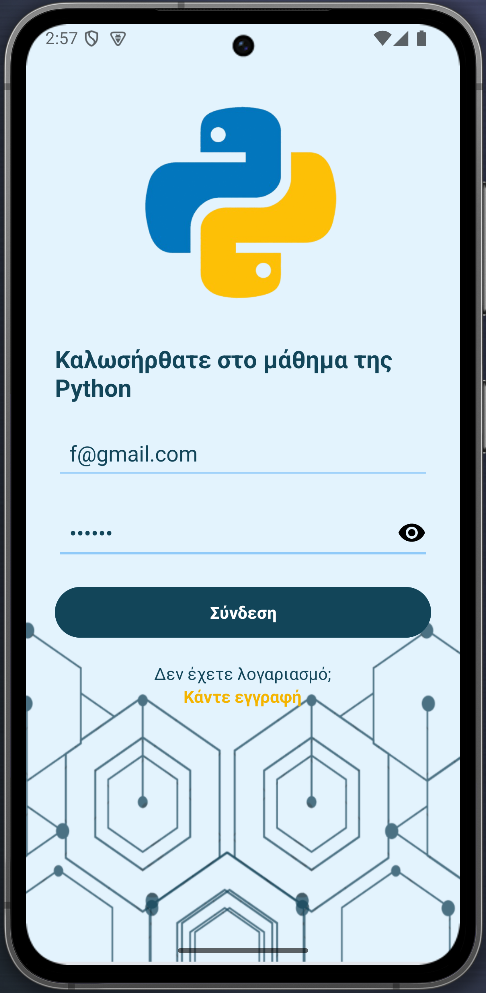
\includegraphics[width=0.9\linewidth, height=0.35\textheight, keepaspectratio]{Figures/s1.png}
  \caption{Οθόνη Σύνδεσης στην Εφαρμογή.}
\end{figure}

\begin{figure}[H]
  \centering
  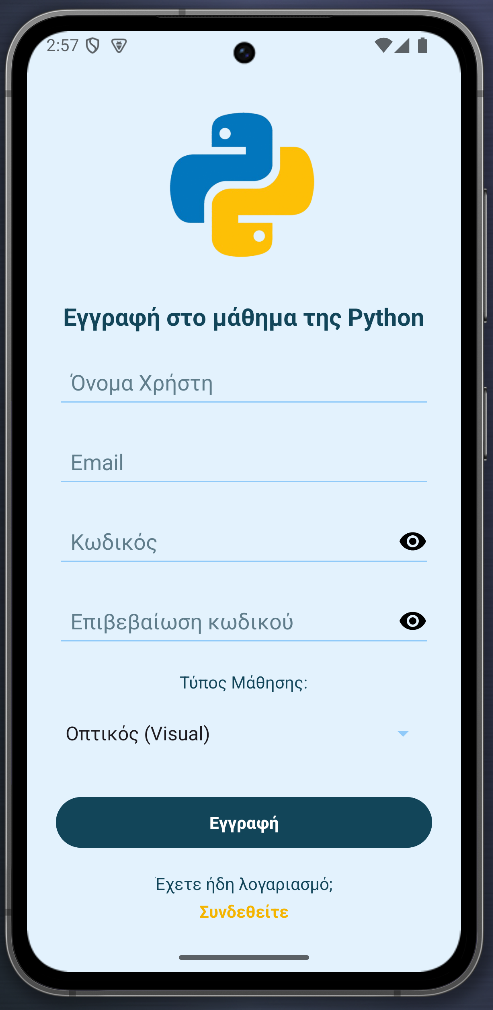
\includegraphics[width=0.9\linewidth, height=0.35\textheight, keepaspectratio]{Figures/s2.png}
  \caption{Οθόνη Εγγραφής Χρήστη στην Εκπαιδευτική Εφαρμογή Python.}
\end{figure}

\begin{figure}[H]
  \centering
  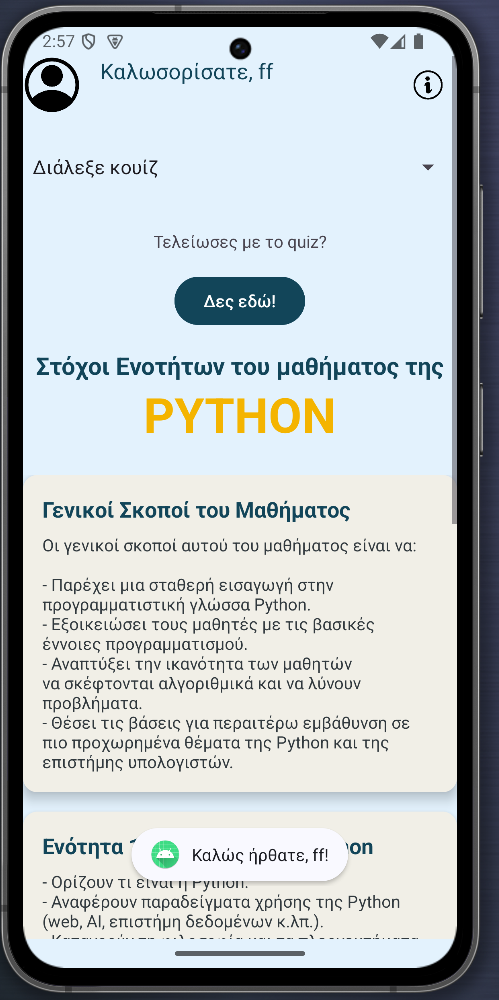
\includegraphics[width=0.9\linewidth, height=0.35\textheight, keepaspectratio]{Figures/s3.png}
  \caption{Κεντρική Σελίδα Εφαρμογής με Γενικούς Σκοπούς Μαθήματος και Ενότητες.}
\end{figure}

\begin{figure}[H]
  \centering
  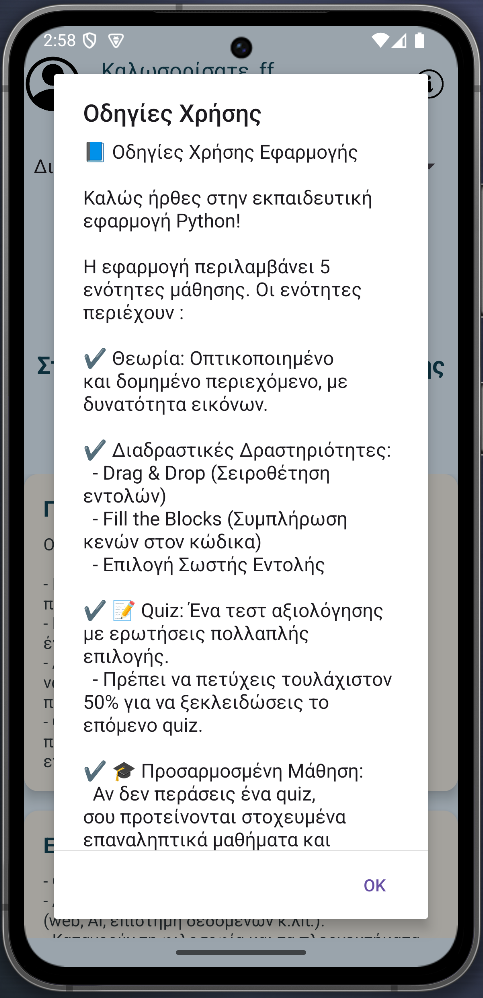
\includegraphics[width=0.9\linewidth, height=0.35\textheight, keepaspectratio]{Figures/s4.png}
  \caption{Οδηγίες Χρήσης Εφαρμογής και Περιγραφή Δραστηριοτήτων.}
\end{figure}

\begin{figure}[H]
  \centering
  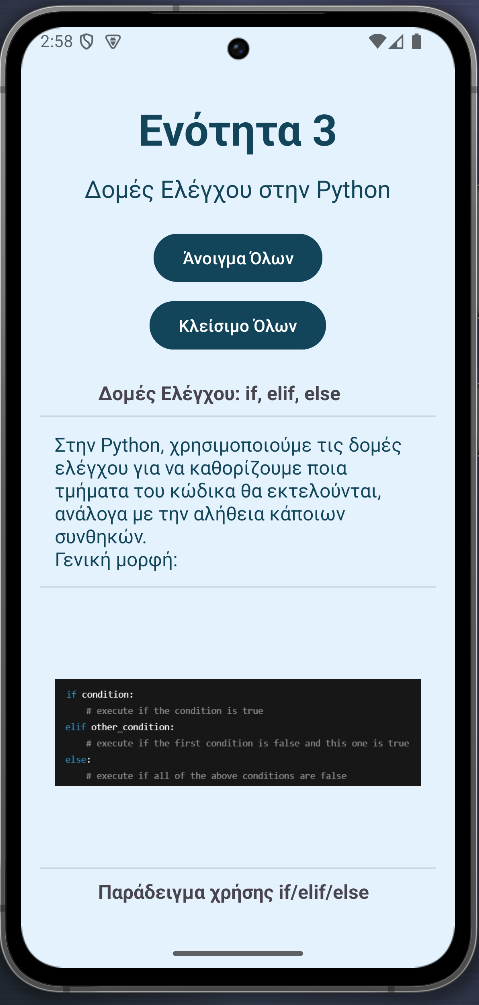
\includegraphics[width=0.9\linewidth, height=0.35\textheight, keepaspectratio]{Figures/s5.png}
  \caption{Ενότητα 3: Δομές Ελέγχου στην Python με Παράδειγμα Κώδικα.}
\end{figure}

\begin{figure}[H]
  \centering
  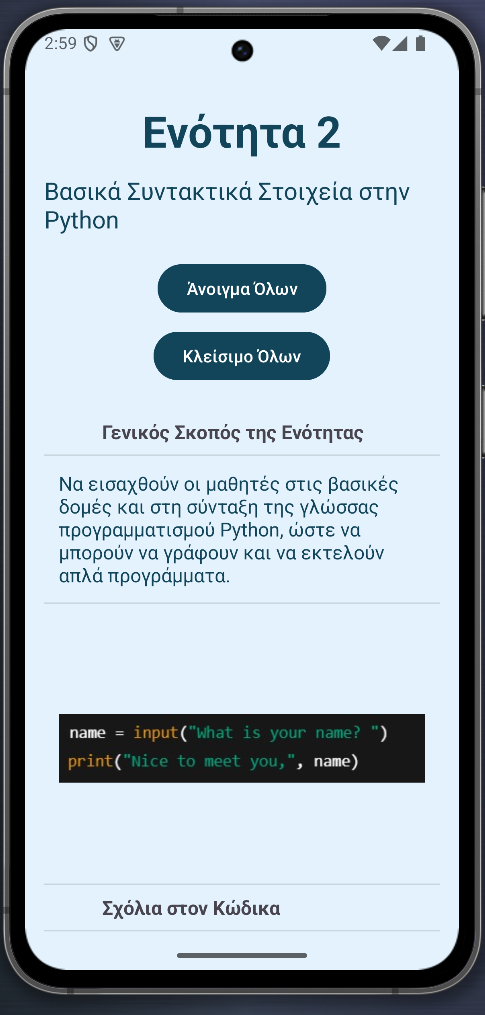
\includegraphics[width=0.9\linewidth, height=0.35\textheight, keepaspectratio]{Figures/s6.png}
  \caption{Παράδειγμα Ενότητας 2.}
\end{figure}

\begin{figure}[H]
  \centering
  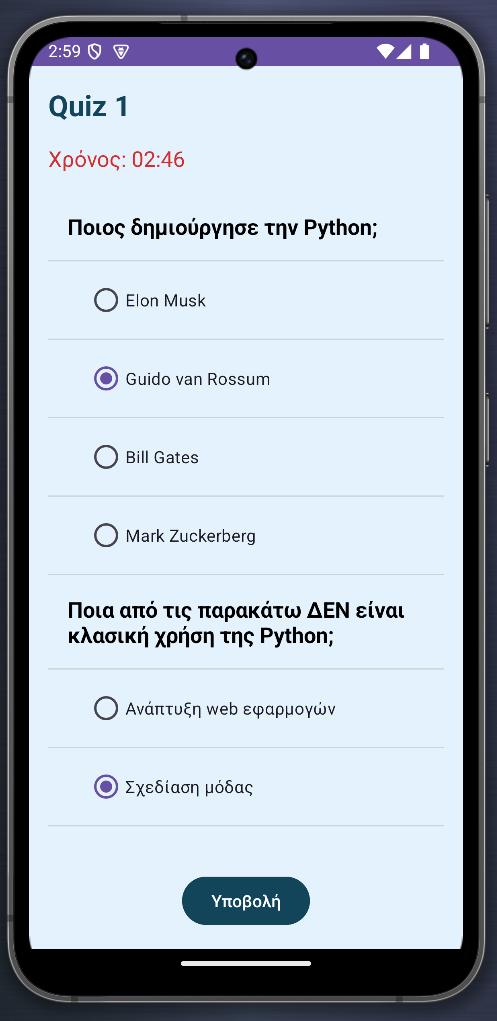
\includegraphics[width=0.9\linewidth, height=0.35\textheight, keepaspectratio]{Figures/s7.png}
  \caption{Οθόνη Quiz 1: Παράδειγμα Αξιολόγησης με Πολλαπλή Επιλογή.}
\end{figure}

\begin{figure}[H]
  \centering
  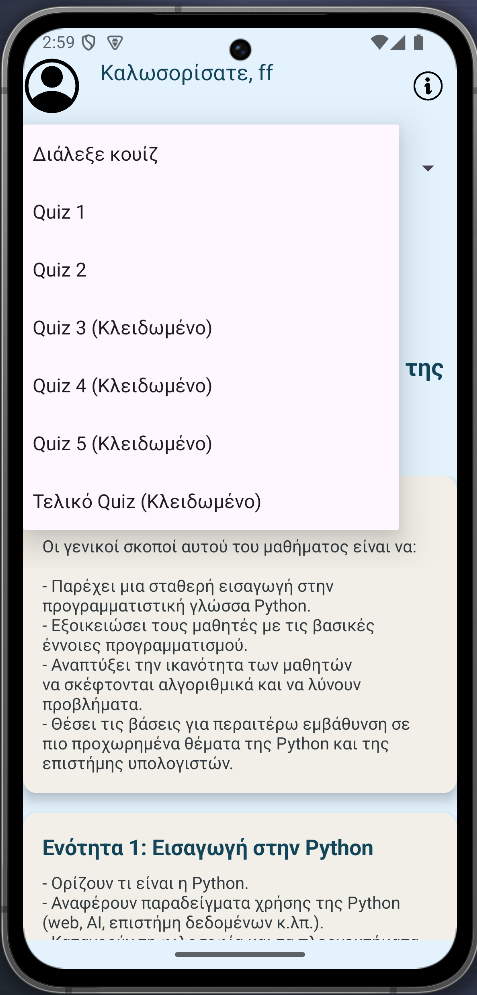
\includegraphics[width=0.9\linewidth, height=0.35\textheight, keepaspectratio]{Figures/s8.png}
  \caption{Λίστα Quiz στην Εφαρμογή και Διαχείριση Πρόσβασης.}
\end{figure}

\begin{figure}[H]
  \centering
  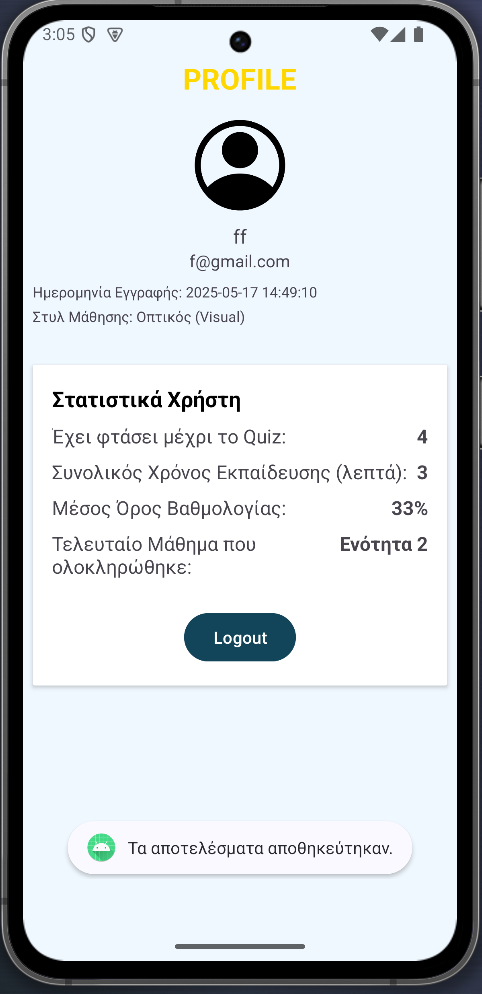
\includegraphics[width=0.9\linewidth, height=0.35\textheight, keepaspectratio]{Figures/s9.png}
  \caption{Οθόνη Στατιστικών Χρήστη με Προσωπικά Εκπαιδευτικά Δεδομένα.}
\end{figure}

\begin{figure}[H]
  \centering
  \begin{minipage}[b]{0.9\linewidth}
    \centering
    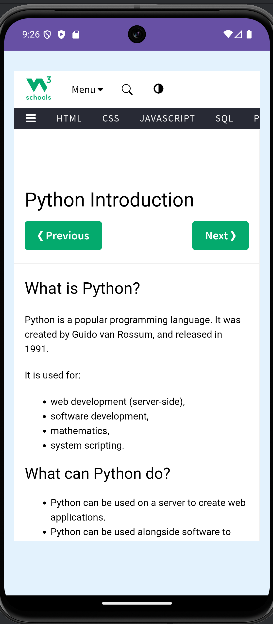
\includegraphics[width=\linewidth, height=0.35\textheight, keepaspectratio]{Figures/εικόνα (1).png}
    \caption{Ενότητα 1: Θεωρητικός και οπτικός μαθητής με επιτυχία στο quiz. Προβάλλεται εμπλουτισμένο θεωρητικό περιεχόμενο μέσω ιστοσελίδας.}
  \end{minipage}
  
  \vspace{0.5cm}

  \begin{minipage}[b]{0.9\linewidth}
    \centering
    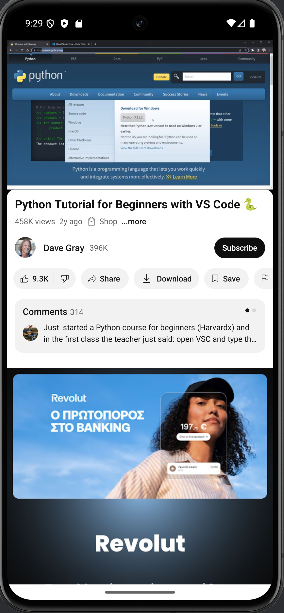
\includegraphics[width=\linewidth, height=0.35\textheight, keepaspectratio]{Figures/εικόνα (2).png}
    \caption{Ενότητα 1: Οπτικός μαθητής με αποτυχία στο quiz. Εμφανίζεται υποστηρικτικό οπτικοακουστικό υλικό (βίντεο YouTube).}
  \end{minipage}
\end{figure}

\begin{figure}[H]
  \centering
  \begin{minipage}[b]{0.45\textwidth}
    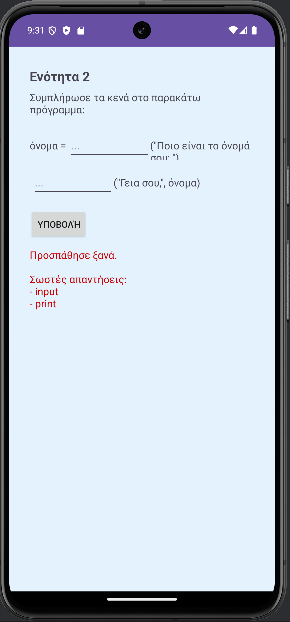
\includegraphics[width=\linewidth, height=0.35\textheight, keepaspectratio]{Figures/εικόνα (3).png}
    \caption{Ενότητα 2: Οπτικός μαθητής με λανθασμένες απαντήσεις και ανατροφοδότηση μέσω σωστών λύσεων.}
  \end{minipage}
  \hfill
  \begin{minipage}[b]{0.45\textwidth}
    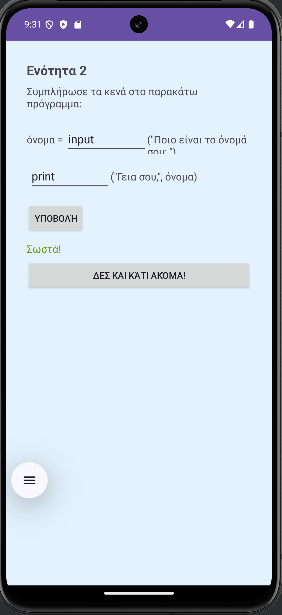
\includegraphics[width=\linewidth, height=0.35\textheight, keepaspectratio]{Figures/εικόνα (4).png}
    \caption{Ενότητα 2: Οπτικός μαθητής με σωστές απαντήσεις στη δραστηριότητα τύπου Fill the Blocks.}
  \end{minipage}
\end{figure}

\begin{figure}[H]
  \centering
  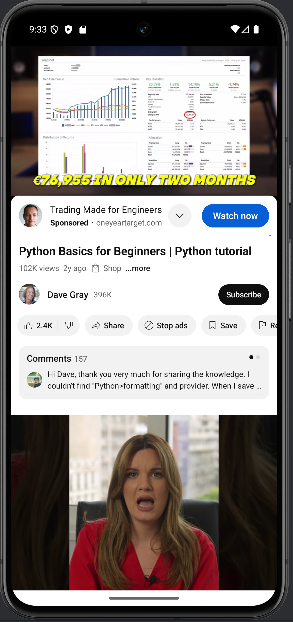
\includegraphics[width=\linewidth, height=0.35\textheight, keepaspectratio]{Figures/εικόνα (5).png}
  \caption{Ενότητα 2: Οπτικός μαθητής με αποτυχία στο quiz. Προτείνεται νέο υποστηρικτικό βίντεο.}
\end{figure}

\begin{figure}[H]
  \centering
  \begin{minipage}[b]{0.45\textwidth}
    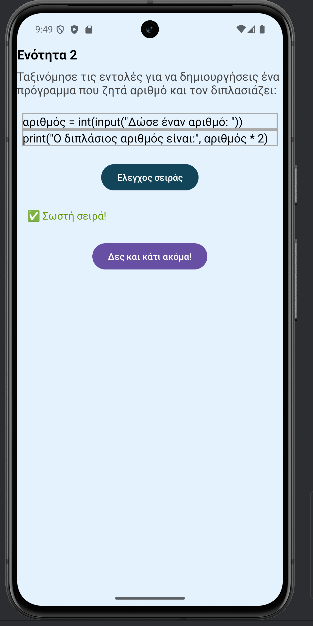
\includegraphics[width=\linewidth, height=0.35\textheight, keepaspectratio]{Figures/εικόνα (16).png}
    \caption{Ενότητα 2: Θεωρητικός μαθητής με επιτυχία στην ορθή σειρά εντολών. Εμφανίζεται μήνυμα επιτυχίας.}
  \end{minipage}
  \hfill
  \begin{minipage}[b]{0.45\textwidth}
    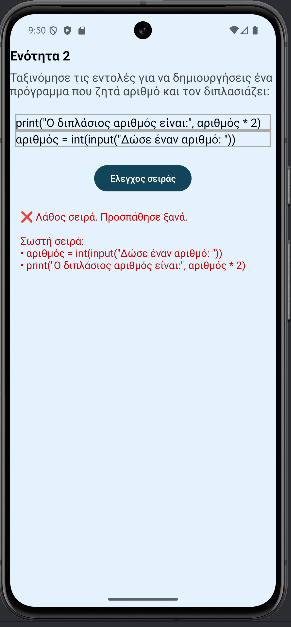
\includegraphics[width=\linewidth, height=0.35\textheight, keepaspectratio]{Figures/εικόνα (17).png}
    \caption{Ενότητα 2: Θεωρητικός μαθητής με αποτυχία στην ορθή σειρά εντολών για διπλασιασμό αριθμού. Προβάλλεται η σωστή λύση.}
  \end{minipage}
\end{figure}

\begin{figure}[H]
  \centering
  \begin{minipage}[b]{0.45\textwidth}
    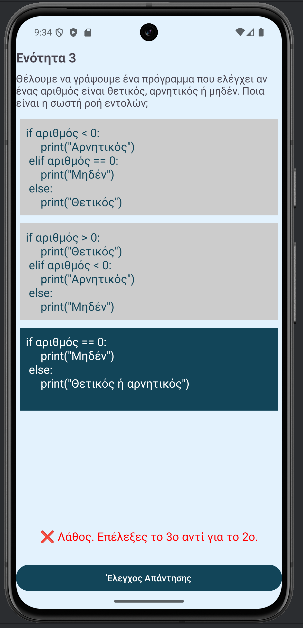
\includegraphics[width=\linewidth, height=0.35\textheight, keepaspectratio]{Figures/εικόνα (6).png}
    \caption{Ενότητα 3: Οπτικός μαθητής με αποτυχία στο quiz. Εμφανίζεται μήνυμα λάθους.}
  \end{minipage}
  \hfill
  \begin{minipage}[b]{0.45\textwidth}
    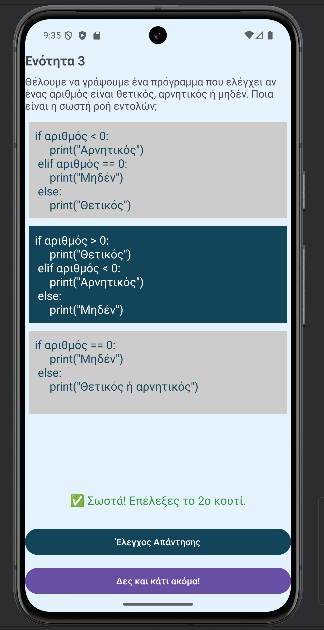
\includegraphics[width=\linewidth, height=0.35\textheight, keepaspectratio]{Figures/εικόνα (7).png}
    \caption{Ενότητα 3: Οπτικός μαθητής με επιτυχία στο quiz. Εμφανίζεται επιβεβαίωση σωστής απάντησης.}
  \end{minipage}
\end{figure}

\begin{figure}[H]
  \centering
  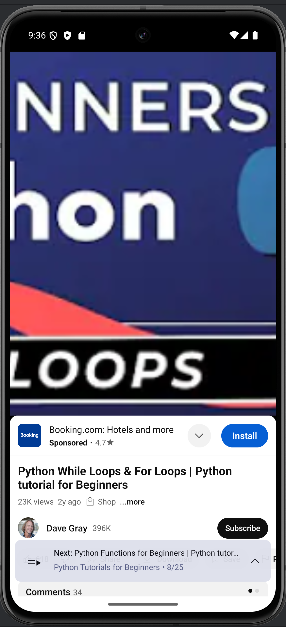
\includegraphics[width=\linewidth, height=0.35\textheight, keepaspectratio]{Figures/εικόνα (8).png}
  \caption{Ενότητα 3: Οπτικός μαθητής με αποτυχία στο quiz. Προτείνεται υποστηρικτικό βίντεο με τίτλο "Python While Loops \& For Loops".}
\end{figure}

\begin{figure}[H]
  \centering
  \begin{minipage}[b]{0.45\textwidth}
    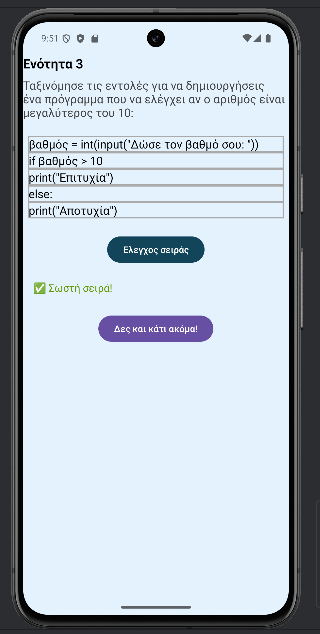
\includegraphics[width=\linewidth, height=0.35\textheight, keepaspectratio]{Figures/εικόνα (18).png}
    \caption{Ενότητα 3: Θεωρητικός μαθητής με επιτυχία στη σύνθεση προγράμματος ελέγχου βαθμού. Εμφανίζεται επιβεβαίωση επιτυχίας.}
  \end{minipage}
  \hfill
  \begin{minipage}[b]{0.45\textwidth}
    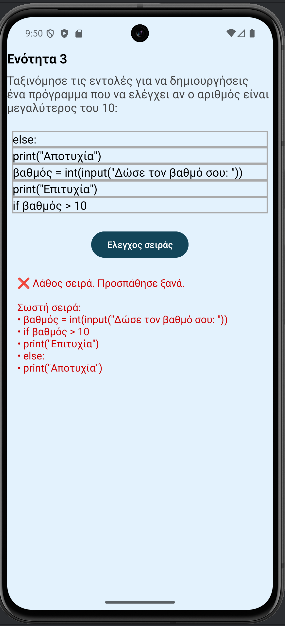
\includegraphics[width=\linewidth, height=0.35\textheight, keepaspectratio]{Figures/εικόνα (19).png}
    \caption{Ενότητα 3: Θεωρητικός μαθητής με αποτυχία στην ταξινόμηση εντολών για έλεγχο βαθμού. Προβάλλεται η σωστή λύση.}
  \end{minipage}
\end{figure}

\begin{figure}[H]
  \centering
  \begin{minipage}[b]{0.45\textwidth}
    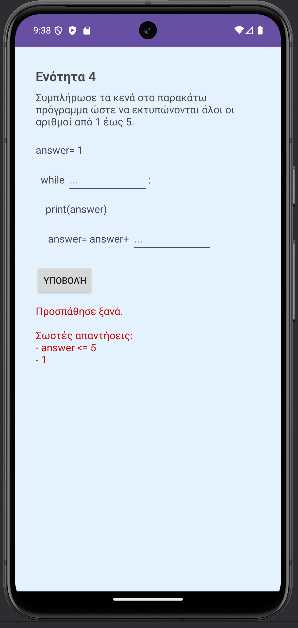
\includegraphics[width=\linewidth, height=0.35\textheight, keepaspectratio]{Figures/εικόνα (9).png}
    \caption{Ενότητα 4: Οπτικός μαθητής με αποτυχία στη συμπλήρωση του προγράμματος. Παρέχεται σωστή απάντηση ως ανατροφοδότηση.}
  \end{minipage}
  \hfill
  \begin{minipage}[b]{0.45\textwidth}
    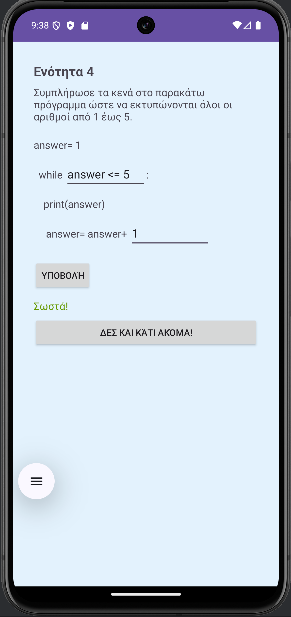
\includegraphics[width=\linewidth, height=0.35\textheight, keepaspectratio]{Figures/εικόνα (10).png}
    \caption{Ενότητα 4: Οπτικός μαθητής με επιτυχία στη συμπλήρωση του προγράμματος επανάληψης (while loop).}
  \end{minipage}
\end{figure}

\begin{figure}[H]
  \centering
  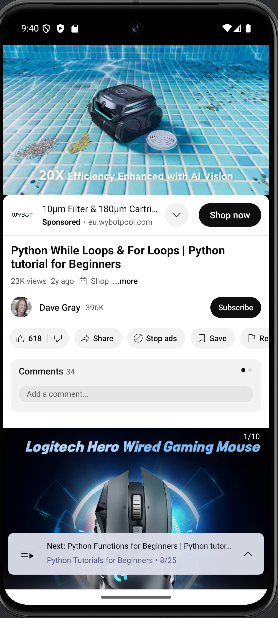
\includegraphics[width=\linewidth, height=0.35\textheight, keepaspectratio]{Figures/εικόνα (11).png}
  \caption{Ενότητα 4: Οπτικός μαθητής με αποτυχία στο quiz. Εμφανίζεται προτεινόμενο βίντεο με τίτλο "Python While Loops \& For Loops".}
\end{figure}

\begin{figure}[H]
  \centering
  \begin{minipage}[b]{0.45\textwidth}
    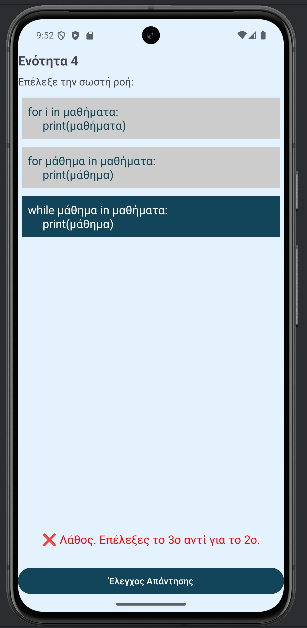
\includegraphics[width=\linewidth, height=0.35\textheight, keepaspectratio]{Figures/εικόνα (20).png}
    \caption{Ενότητα 4: Θεωρητικός μαθητής με αποτυχία στην επιλογή της σωστής εντολής επανάληψης. Εμφανίζεται μήνυμα λάθους.}
  \end{minipage}
  \hfill
  \begin{minipage}[b]{0.45\textwidth}
    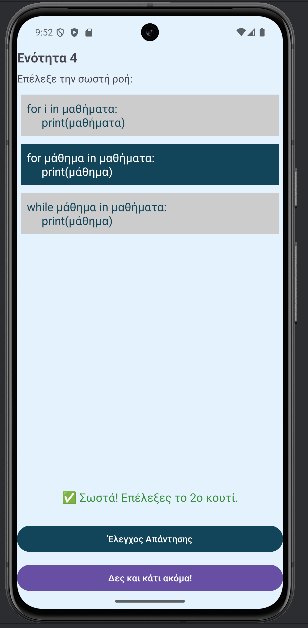
\includegraphics[width=\linewidth, height=0.35\textheight, keepaspectratio]{Figures/εικόνα (21).png}
    \caption{Ενότητα 4: Θεωρητικός μαθητής με επιτυχία στην επιλογή της εντολής \texttt{for} για επανάληψη. Εμφανίζεται μήνυμα επιτυχίας.}
  \end{minipage}
\end{figure}


\begin{figure}[H]
  \centering
  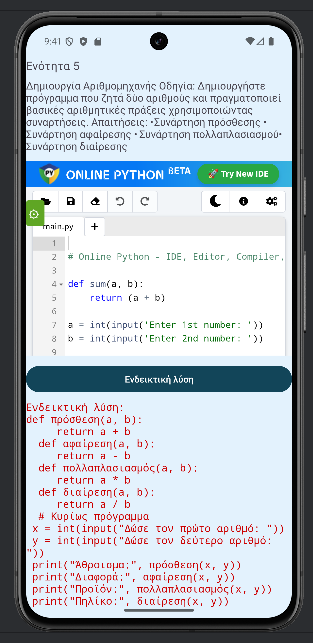
\includegraphics[width=\linewidth, height=0.35\textheight, keepaspectratio]{Figures/εικόνα (12).png}
  \caption{Ενότητα 5: Οπτικός μαθητής με επιτυχία στη δημιουργία αριθμομηχανής με βασικές αριθμητικές πράξεις. Παρέχεται ενδεικτική λύση με χρήση συναρτήσεων.}
\end{figure}

\begin{figure}[H]
  \centering
  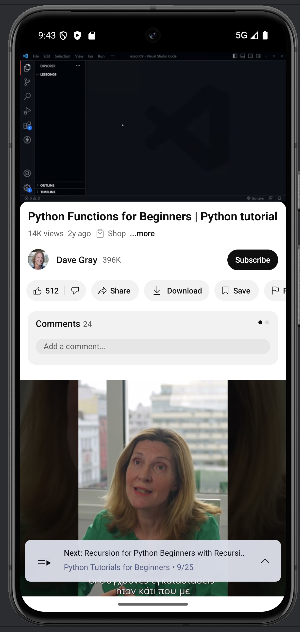
\includegraphics[width=\linewidth, height=0.35\textheight, keepaspectratio]{Figures/εικόνα (13).png}
  \caption{Ενότητα 5: Οπτικός μαθητής με αποτυχία στο quiz. Εμφανίζεται προτεινόμενο υποστηρικτικό βίντεο με τίτλο "Python Functions for Beginners".}
\end{figure}

\begin{figure}[H]
  \centering
  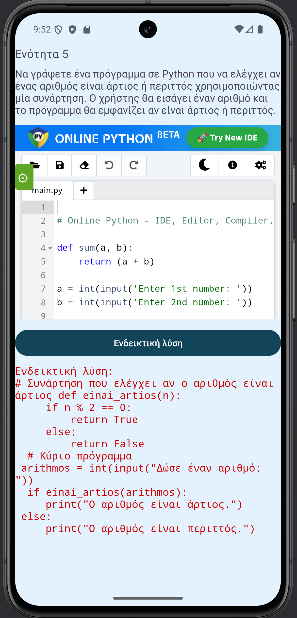
\includegraphics[width=\linewidth, height=0.35\textheight, keepaspectratio]{Figures/εικόνα (22).png}
  \caption{Ενότητα 5: Θεωρητικός μαθητής με επιτυχία. Προβάλλεται ενδεικτική λύση που χρησιμοποιεί συνάρτηση για έλεγχο άρτιου ή περιττού αριθμού.}
\end{figure}

\begin{figure}[H]
  \centering
  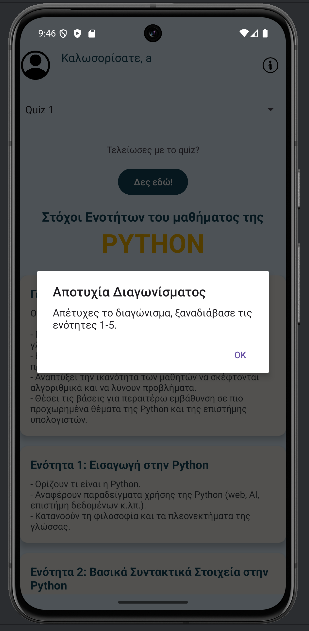
\includegraphics[width=\linewidth, height=0.35\textheight, keepaspectratio]{Figures/εικόνα (14).png}
  \caption{Αποτυχία Διαγωνίσματος: Ο μαθητής απέτυχε στο quiz των Ενοτήτων 1–5 και προτείνεται επαναμελέτη του υλικού.}
\end{figure}

\begin{figure}[H]
  \centering
  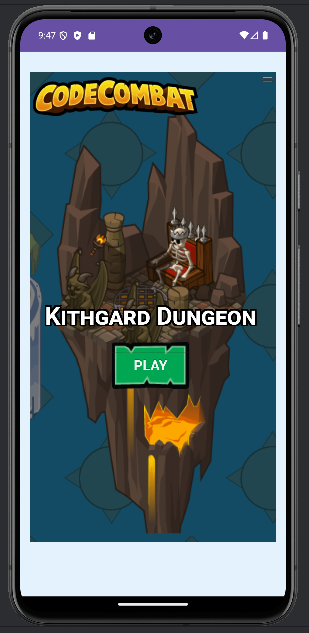
\includegraphics[width=\linewidth, height=0.35\textheight, keepaspectratio]{Figures/εικόνα (15).png}
  \caption{Επιτυχία Διαγωνίσματος: Ο μαθητής ολοκλήρωσε επιτυχώς τις ενότητες και προχωρά σε παιγνιώδη μαθησιακή δραστηριότητα στο περιβάλλον CodeCombat.}
\end{figure}

\chapter{Εκπαιδευτικό Υλικό \& Ασκήσεις (ανά Ενότητα)}
\section{Ενότητες}
Η εκπαιδευτική εφαρμογή είναι οργανωμένη σε πέντε διαδοχικές ενότητες, κάθε μία από τις οποίες εστιάζει σε θεμελιώδη στοιχεία της γλώσσας Python. Η πρώτη ενότητα παρέχει μια γενική εισαγωγή στη γλώσσα και τα πλεονεκτήματά της. Η δεύτερη εισάγει τις βασικές συντακτικές δομές, όπως οι μεταβλητές και οι τύποι δεδομένων. Στην τρίτη ενότητα εξετάζονται οι δομές ελέγχου, δηλαδή οι συνθήκες και η λογική ροή. Η τέταρτη αφορά τις επαναλήψεις και τις λίστες, ενώ η πέμπτη κορυφώνεται με τις συναρτήσεις και ένα mini project δημιουργικής εφαρμογής. Κάθε ενότητα περιλαμβάνει θεωρητικό υλικό, ερωτήσεις αξιολόγησης, διαδραστικές δραστηριότητες, καθώς και εξατομικευμένες διαδρομές μάθησης. 

\subsection{Ενότητα 1: Εισαγωγή στην Python}

\textbf{Γενικός Σκοπός της Ενότητας} \\[0.5em]
Να αποκτήσουν οι μαθητές βασική κατανόηση:

\begin{itemize}
    \item Τι είναι η Python.
    \item Σε ποια πεδία χρησιμοποιείται.
    \item Γιατί είναι σημαντική στον προγραμματισμό σήμερα.
\end{itemize}

\vspace{1em}
\textbf{Αναλυτικοί Διδακτικοί Στόχοι} \\[0.5em]
Μετά την ολοκλήρωση της ενότητας, οι μαθητές θα πρέπει να μπορούν να:

\begin{itemize}
    \item Ορίζουν τι είναι η Python.
    \item Αναφέρουν παραδείγματα χρήσης της Python (web, AI, επιστήμη δεδομένων κ.λπ.).
    \item Κατανοούν τη φιλοσοφία και τα πλεονεκτήματα της γλώσσας (π.χ. απλότητα, αναγνωσιμότητα).
\end{itemize}

\vspace{1em}
\textbf{Εκπαιδευτικό Υλικό} \\

\vspace{0.5em}
\textbf{Τι είναι η Python;} \\[0.5em]
Η Python είναι μία σύγχρονη, υψηλού επιπέδου γλώσσα προγραμματισμού, η οποία δημιουργήθηκε το 1991 από τον Ολλανδό προγραμματιστή Guido van Rossum.

Χαρακτηρίζεται από την απλότητα στη σύνταξη και την ευκολία στην ανάγνωση και κατανόηση του κώδικα, γεγονός που την καθιστά ιδιαίτερα προσιτή τόσο σε αρχάριους όσο και σε έμπειρους προγραμματιστές.

Η Python έχει εξελιχθεί σε μία από τις δημοφιλέστερες γλώσσες προγραμματισμού παγκοσμίως, χρησιμοποιούμενη σε πληθώρα εφαρμογών και τεχνολογικών πεδίων.

\vspace{1em}
\textbf{Περιοχές Χρήσης της Python} \\[0.5em]
Η Python χρησιμοποιείται εκτενώς σε διάφορους τομείς, όπως:

\begin{itemize}
    \item \textbf{Ανάπτυξη Ιστοσελίδων και Εφαρμογών (Web Development):} Δημιουργία δυναμικών ιστότοπων και διαδικτυακών υπηρεσιών.
    \item \textbf{Επιστήμη Δεδομένων (Data Science):} Ανάλυση και επεξεργασία μεγάλων όγκων δεδομένων.
    \item \textbf{Μηχανική Μάθηση και Τεχνητή Νοημοσύνη (Machine Learning \& AI):} Ανάπτυξη "έξυπνων" συστημάτων που βασίζονται σε δεδομένα.
    \item \textbf{Αυτοματισμός Εργασιών (Automation):} Αυτοματοποίηση επαναλαμβανόμενων ή πολύπλοκων διαδικασιών.
    \item \textbf{Ανάπτυξη Παιχνιδιών (Game Development):} Δημιουργία ψηφιακών παιχνιδιών και εφαρμογών διασκέδασης.
    \item \textbf{Internet of Things (IoT):} Ανάπτυξη εφαρμογών για έξυπνες συσκευές και αισθητήρες.
\end{itemize}

\vspace{1em}
\textbf{Πλεονεκτήματα της Python} \\[0.5em]
Η Python παρουσιάζει σημαντικά πλεονεκτήματα έναντι άλλων γλωσσών προγραμματισμού, μεταξύ των οποίων:

\begin{itemize}
    \item \textbf{Απλότητα και Αναγνωσιμότητα:} Ο κώδικας είναι ευανάγνωστος και μοιάζει με την αγγλική γλώσσα.
    \item \textbf{Ευκολία Εκμάθησης:} Ιδανική επιλογή για μαθητές και αρχάριους προγραμματιστές.
    \item \textbf{Πολυχρηστικότητα:} Εφαρμόζεται σε πληθώρα τομέων της πληροφορικής και της τεχνολογίας.
    \item \textbf{Δυνατότητα Επαγγελματικής Ανάπτυξης:} Μεγάλη ζήτηση στην αγορά εργασίας.
    \item \textbf{Υποστήριξη μέσω Κοινότητας και Βιβλιοθηκών:} Πλούσια διαθέσιμη τεκμηρίωση και πληθώρα έτοιμων εργαλείων.
\end{itemize}

\vspace{1em}
\textbf{Ιστορικό Πλαίσιο} \\[0.5em]

Η Python οφείλει το όνομά της στην κωμική ομάδα \textit{Monty Python’s Flying Circus}, γεγονός που αντανακλά την πρόθεση του δημιουργού της για έναν προγραμματισμό ευχάριστο και απλό.

Παρά το φιλικό της προφίλ, η Python έχει ισχυρές δυνατότητες και χρησιμοποιείται σε απαιτητικά επαγγελματικά έργα.

\vspace{1em}
\textbf{Σύνοψη της Ενότητας} \\[0.5em]
Με την ολοκλήρωση της παρούσας ενότητας, οι μαθητές αναμένεται να:

\begin{itemize}
    \item Κατανοούν τι είναι η γλώσσα προγραμματισμού Python.
    \item Αναγνωρίζουν τους βασικούς τομείς εφαρμογής της.
    \item Εκτιμούν τα κύρια πλεονεκτήματα και τα χαρακτηριστικά της.
\end{itemize}

\vspace{1em}
\textbf{Δραστηριότητες – Ερωτήσεις Αυτοαξιολόγησης} \\[0.5em]
\textbf{Quiz Πολλαπλής Επιλογής}
\begin{enumerate}
    \item \textbf{Ποιος δημιούργησε την Python;}
    \begin{itemize}
        \item[A)] Elon Musk
        \item[B)] \textbf{Guido van Rossum}
        \item[C)] Bill Gates
        \item[D)] Mark Zuckerberg
    \end{itemize}

    \item \textbf{Ποια από τις παρακάτω \underline{ΔΕΝ} είναι κλασική χρήση της Python;}
    \begin{itemize}
        \item[A)] Ανάπτυξη web εφαρμογών
        \item[B)] \textbf{Σχεδίαση μόδας}
        \item[C)] Επιστήμη δεδομένων
        \item[D)] Τεχνητή Νοημοσύνη
    \end{itemize}

    \item \textbf{Ποιο από τα παρακάτω \underline{ΔΕΝ} αποτελεί πλεονέκτημα της Python;}
    \begin{itemize}
        \item[A)] Ευκολία στη μάθηση
        \item[B)] Μεγάλη κοινότητα υποστήριξης
        \item[C)] \textbf{Δύσκολη σύνταξη}
        \item[D)] Πολλές έτοιμες βιβλιοθήκες
    \end{itemize}
\end{enumerate}


\subsection{Ενότητα 2: Βασικά Συντακτικά Στοιχεία στην Python}

\textbf{Γενικός Σκοπός της Ενότητας} \\
Να εισαχθούν οι μαθητές στις βασικές δομές και στη σύνταξη της γλώσσας προγραμματισμού Python, ώστε να μπορούν να γράφουν και να εκτελούν απλά προγράμματα.

\vspace{1em}

\textbf{Αναλυτικοί Διδακτικοί Στόχοι} \\
Μετά την ολοκλήρωση της ενότητας, οι μαθητές θα πρέπει να μπορούν να:
\begin{itemize}
    \item Δημιουργούν και να χρησιμοποιούν μεταβλητές στην Python.
    \item Αναγνωρίζουν και να χειρίζονται βασικούς τύπους δεδομένων.
    \item Χρησιμοποιούν εντολές εισόδου και εξόδου (input/output).
    \item Κατανοούν τη σημασία των σχολίων στον κώδικα.
\end{itemize}

\vspace{1em}

\textbf{Εκπαιδευτικό Υλικό}

\textbf{Μεταβλητές στην Python} \\
Στην Python, μεταβλητές είναι θέσεις αποθήκευσης δεδομένων, που χρησιμοποιούνται για να κρατούν τιμές.\\
Παράδειγμα:

\begin{tcolorbox}[colback=gray!5!white, colframe=black!75!black]
x = 5 \\
όνομα = "Μαρία"
\end{tcolorbox}

Σημαντικά σημεία:
\begin{itemize}
    \item Δεν χρειάζεται να δηλώσουμε τύπο μεταβλητής (η Python τον αναγνωρίζει αυτόματα).
    \item Το όνομα της μεταβλητής πρέπει να ξεκινά με γράμμα ή κάτω παύλα (\_).
\end{itemize}

\vspace{1em}

\textbf{Βασικοί Τύποι Δεδομένων} \\
Στην Python συναντάμε βασικούς τύπους δεδομένων, όπως:

\begin{itemize}
    \item \textbf{Ακέραιοι αριθμοί (int):} π.χ. 10
    \item \textbf{Δεκαδικοί αριθμοί (float):} π.χ. 3.14
    \item \textbf{Συμβολοσειρές (string):} π.χ. ``Καλημέρα''
    \item \textbf{Λογικές τιμές (boolean):} \texttt{True} ή \texttt{False}
\end{itemize}
Παραδείγματα:

\begin{tcolorbox}[colback=gray!5!white, colframe=black!75!black]
ηλικία = 17 \\
ύψος = 1.75 \\
όνομα = "Γιάννης" \\
είναι\_μαθητής = True
\end{tcolorbox}

\vspace{1em}

\subsection*{Είσοδος και Έξοδος Δεδομένων}

Η Python παρέχει εύκολους τρόπους εισαγωγής και εμφάνισης δεδομένων.

\vspace{1em}
\textbf{Εμφάνιση στην οθόνη (Έξοδος):}

\begin{tcolorbox}[colback=gray!5!white, colframe=black!75!black]
\texttt{print("Καλωσήρθατε στον κόσμο της Python!")}
\end{tcolorbox}

\vspace{1em}
\textbf{Εισαγωγή δεδομένων από τον χρήστη (Είσοδος):}

\begin{tcolorbox}[colback=gray!5!white, colframe=black!75!black]
\texttt{όνομα = input("Ποιο είναι το όνομά σου;")} \\
\texttt{print("Χαίρω πολύ,", όνομα)}
\end{tcolorbox}

\vspace{1em}
Το \texttt{input()} επιστρέφει πάντα \texttt{string}, ακόμη κι αν ο χρήστης εισάγει αριθμό.

\vspace{1em}
\textbf{Σχόλια στον κώδικα}

Τα σχόλια χρησιμοποιούνται για να εξηγούν τι κάνει ο κώδικας και αγνοούνται κατά την εκτέλεση.

\vspace{1em}
\textbf{Για μονή γραμμή σχολίου:}

\begin{tcolorbox}[colback=gray!5!white, colframe=black!75!black]
\texttt{\# Αυτό είναι ένα σχόλιο}
\end{tcolorbox}

\vspace{1em}
\textbf{Για πολλαπλές γραμμές σχολίου:}

\begin{tcolorbox}[colback=gray!5!white, colframe=black!75!black]
\texttt{"""}

\texttt{Αυτό είναι ένα}

\texttt{σχόλιο πολλών γραμμών.}

\texttt{"""}
\end{tcolorbox}

\vspace{1em}
Η χρήση σχολίων κάνει τον κώδικα ευανάγνωστο και πιο εύκολο στη συντήρηση.

\vspace{1em}
\textbf{Σύνοψη της Ενότητας} \\[0.5em]
Με την ολοκλήρωση της παρούσας ενότητας, οι μαθητές αναμένεται να:

\begin{itemize}
    \item Δημιουργούν και να χρησιμοποιούν βασικές μεταβλητές και τύπους δεδομένων.
    \item Χρησιμοποιούν εντολές εισόδου και εξόδου στην Python.
    \item Κατανοούν τη σημασία των σχολίων στον προγραμματισμό.
\end{itemize}

\subsection*{Δραστηριότητες – Ερωτήσεις Αυτοαξιολόγησης}
\textbf{Quiz Πολλαπλής Επιλογής (Multiple Choice)} 

\vspace{1em}
\textbf{Ερώτηση 1:} Ποια εντολή χρησιμοποιούμε για να εμφανίσουμε κείμενο στην Python;

\begin{itemize}
    \item Ερώτηση 1: Ποια εντολή χρησιμοποιούμε για να εμφανίσουμε κείμενο στην Python;
    \begin{itemize}
        \item[A)] \texttt{input()}
        \item[B)] \texttt{show()}
        \item[C)] \textbf{\texttt{print()}}
        \item[D)] \texttt{display()}
    \end{itemize}

    \item Ερώτηση 2: Τι τύπο δεδομένων επιστρέφει πάντα η εντολή \texttt{input();};
    \begin{itemize}
        \item[A)] Ακέραιο (int)
        \item[B)] Δεκαδικό (float)
        \item[C)] \textbf{Συμβολοσειρά (string)}
        \item[D)] Λογική τιμή (boolean)
    \end{itemize}

    \item Ερώτηση 3: Ποιο από τα παρακάτω είναι σωστός τρόπος δημιουργίας σχολίου στην Python;
    \begin{itemize}
        \item[A)] \texttt{/* Σχόλιο */}
        \item[B)] \textbf{\texttt{\# Σχόλιο}}
        \item[C)] \texttt{// Σχόλιο}
        \item[D)] \texttt{<!-- Σχόλιο -->}
    \end{itemize}
\end{itemize}

\vspace{1em}
\textbf{Ερώτηση 2:} Τι τύπο δεδομένων επιστρέφει πάντα η εντολή \texttt{input();}

\begin{itemize}
    \item Ερώτηση 1: Ποια εντολή χρησιμοποιούμε για να εμφανίσουμε κείμενο στην Python;
    \begin{itemize}
        \item[A)] \texttt{input()}
        \item[B)] \texttt{show()}
        \item[C)] \textbf{\texttt{print()}}
        \item[D)] \texttt{display()}
    \end{itemize}

    \item Ερώτηση 2: Τι τύπο δεδομένων επιστρέφει πάντα η εντολή \texttt{input();};
    \begin{itemize}
        \item[A)] Ακέραιο (int)
        \item[B)] Δεκαδικό (float)
        \item[C)] \textbf{Συμβολοσειρά (string)}
        \item[D)] Λογική τιμή (boolean)
    \end{itemize}

    \item Ερώτηση 3: Ποιο από τα παρακάτω είναι σωστός τρόπος δημιουργίας σχολίου στην Python;
    \begin{itemize}
        \item[A)] \texttt{/* Σχόλιο */}
        \item[B)] \textbf{\texttt{\# Σχόλιο}}
        \item[C)] \texttt{// Σχόλιο}
        \item[D)] \texttt{<!-- Σχόλιο -->}
    \end{itemize}
\end{itemize}

\textbf{Άσκηση Συμπλήρωσης Κώδικα (Fill-in-the-Blank) (Οπτικός)}

\textbf{Οδηγία:} Συμπλήρωσε τα κενά στο παρακάτω πρόγραμμα.

\begin{tcolorbox}[colback=white, colframe=black!75!black]
\# Το πρόγραμμα ζητά από τον χρήστη το όνομά του και το εμφανίζει.

όνομα = \_\_\_\_\_\_\_\_\_\_\_("Ποιο είναι το όνομά σου; ")

\_\_\_\_\_\_\_\_\_\_\_("Γεια σου,", όνομα)
\end{tcolorbox}

\textbf{Σωστές απαντήσεις:}
\begin{itemize}
    \item Πρώτο κενό: \texttt{input}
    \item Δεύτερο κενό: \texttt{print}
\end{itemize}

\vspace{1em}
\noindent\rule{\linewidth}{0.4pt}

\vspace{1em}

\textbf{Drag \& Drop (Ταξινόμηση Λογικών Βημάτων) (Θεωρητικός)}

\textbf{Οδηγία:} Ταξινόμησε τις εντολές για να δημιουργήσεις ένα πρόγραμμα που ζητά αριθμό και τον διπλασιάζει.

\textbf{Κομμάτια Κώδικα:}
\begin{itemize}
    \item \texttt{print("Ο διπλάσιος αριθμός είναι:", αριθμός * 2)}
    \item \texttt{αριθμός = int(input("Δώσε έναν αριθμό: "))}
\end{itemize}

\textbf{Σωστή σειρά:}
\begin{enumerate}
    \item \texttt{αριθμός = int(input("Δώσε έναν αριθμό: "))}
    \item \texttt{print("Ο διπλάσιος αριθμός είναι:", αριθμός * 2)}
\end{enumerate}

\subsection{Ενότητα 3: Δομές Ελέγχου Ροής στην Python}

\textbf{Γενικός Σκοπός της Ενότητας} \\[0.5em]
Να εισαχθούν οι μαθητές στις βασικές δομές ελέγχου ροής της γλώσσας \textbf{Python}, οι οποίες επιτρέπουν στον κώδικα να λαμβάνει αποφάσεις και να εκτελεί διαφορετικές ενέργειες με βάση συνθήκες.

\vspace{1em}
\textbf{Αναλυτικοί Διδακτικοί Στόχοι} \\[0.5em]
Μετά την ολοκλήρωση της ενότητας, οι μαθητές θα πρέπει να μπορούν να:

\begin{itemize}
    \item Χρησιμοποιούν τις εντολές \texttt{if}, \texttt{elif}, \texttt{else} για έλεγχο ροής προγραμμάτων.
    \item Κατανοούν και να εφαρμόζουν λογικούς τελεστές (\texttt{and}, \texttt{or}, \texttt{not}).
    \item Δημιουργούν απλά προγράμματα με συνθήκες και επιλογές.
\end{itemize}

\vspace{1em}
\textbf{Εκπαιδευτικό Υλικό} \\

\textbf{Δομές Ελέγχου: \texttt{if}, \texttt{elif}, \texttt{else}} \\[0.5em]
Στην \textbf{Python}, χρησιμοποιούμε τις δομές ελέγχου για να καθορίζουμε ποια τμήματα του κώδικα θα εκτελούνται, ανάλογα με την αλήθεια κάποιων συνθηκών.

\textbf{Γενική μορφή:}
\begin{tcolorbox}[colback=gray!5!white, colframe=black!75!black]
\begin{verbatim}
if συνθήκη:
    # εκτέλεση αν η συνθήκη είναι αληθής
elif άλλη_συνθήκη:
    # εκτέλεση αν η πρώτη συνθήκη είναι ψευδής και αυτή αληθής
else:
    # εκτέλεση αν όλες οι παραπάνω συνθήκες είναι ψευδείς
\end{verbatim}
\end{tcolorbox}

\textbf{Παράδειγμα:}
\begin{tcolorbox}[colback=gray!5!white, colframe=black!75!black]
\begin{verbatim}
βαθμός = 18

if βαθμός >= 18:
    print("Άριστα")
elif βαθμός >= 10:
    print("Επιτυχία")
else:
    print("Αποτυχία")
\end{verbatim}
\end{tcolorbox}

\vspace{1em}
\textbf{Λογικοί Τελεστές}

Οι λογικοί τελεστές χρησιμοποιούνται για τη σύνθεση πολλαπλών συνθηκών:

\begin{tabular}{|l|l|l|}
\hline
\textbf{Τελεστής} & \textbf{Περιγραφή} & \textbf{Παράδειγμα} \\
\hline
\texttt{and} & Αληθές αν και οι δύο συνθήκες είναι αληθείς & \texttt{x > 5 and x < 10} \\
\texttt{or}  & Αληθές αν τουλάχιστον μία συνθήκη είναι αληθής & \texttt{x < 5 or x > 15} \\
\texttt{not} & Αντιστροφή της λογικής τιμής & \texttt{not(x > 10)} \\
\hline
\end{tabular}

\vspace{1em}
\textbf{Παράδειγμα χρήσης:}
\begin{tcolorbox}[colback=gray!5!white, colframe=black!75!black]
\begin{verbatim}
ηλικία = 20

if ηλικία >= 18 and ηλικία <= 65:
    print("Ενήλικας σε παραγωγική ηλικία")
\end{verbatim}
\end{tcolorbox}

\vspace{1em}
\textbf{Σύνοψη της Ενότητας} \\[0.5em]
Με την ολοκλήρωση της παρούσας ενότητας, οι μαθητές αναμένεται να:

\begin{itemize}
    \item Δημιουργούν προγράμματα που λαμβάνουν αποφάσεις με συνθήκες.
    \item Συνδυάζουν πολλαπλές συνθήκες χρησιμοποιώντας λογικούς τελεστές.
    \item Εφαρμόζουν σωστή λογική ροή στο πρόγραμμά τους.
\end{itemize}

\vspace{1em}
\textbf{Δραστηριότητες – Ερωτήσεις Αυτοαξιολόγησης} \\[0.5em]
\textbf{Quiz Πολλαπλής Επιλογής}
\begin{enumerate}
    \item \textbf{Ποια εντολή χρησιμοποιείται για να ελέγξουμε μία συνθήκη στην \texttt{Python};}
    \begin{itemize}
        \item[A)] loop
        \item[B)] print
        \item[C)] \textbf{if}
        \item[D)] input
    \end{itemize}

    \item \textbf{Τι εκτελεί το πρόγραμμα αν καμία από τις συνθήκες \texttt{if} ή \texttt{elif} δεν είναι αληθής;}
    \begin{itemize}
        \item[A)] Αγνοεί το υπόλοιπο πρόγραμμα.
        \item[B)] \textbf{Εκτελεί το else.}
        \item[C)] Κλείνει το πρόγραμμα.
        \item[D)] Εμφανίζει σφάλμα.
    \end{itemize}

    \item \textbf{Ποιος τελεστής χρησιμοποιείται για να αντιστρέψουμε μία λογική συνθήκη;}
    \begin{itemize}
        \item[A)] and
        \item[B)] or
        \item[C)] \textbf{not}
        \item[D)] if
    \end{itemize}
\end{enumerate}

\vspace{1em}
\textbf{Ασκήσεις – Επιλογής Σωστής Ροής (Flow Choice)} \\[0.5em]
\textbf{Άσκηση 1:} \\
Θέλουμε να γράψουμε ένα πρόγραμμα που ελέγχει αν ένας αριθμός είναι θετικός, αρνητικός ή μηδέν.\\
Ποια είναι η σωστή ροή εντολών;

\textbf{A)}
\begin{tcolorbox}[colback=gray!5!white, colframe=black!75!black]
\begin{verbatim}
if αριθμός < 0:
    print("Αρνητικός")
elif αριθμός == 0:
    print("Μηδέν")
else:
    print("Θετικός")
\end{verbatim}
\end{tcolorbox}

\textbf{B)}
\begin{tcolorbox}[colback=gray!5!white, colframe=black!75!black]
\begin{verbatim}
if αριθμός > 0:
    print("Θετικός")
elif αριθμός < 0:
    print("Αρνητικός")
else:
    print("Μηδέν")
\end{verbatim}
\end{tcolorbox}

\textbf{C)}
\begin{tcolorbox}[colback=gray!5!white, colframe=black!75!black]
\begin{verbatim}
if αριθμός == 0:
    print("Μηδέν")
else:
    print("Θετικός ή αρνητικός")
\end{verbatim}
\end{tcolorbox}

\textit{Σωστή απάντηση: \textbf{B} (Ελέγχουμε πρώτα αν είναι θετικός, μετά αν είναι αρνητικός, αλλιώς είναι μηδέν.)}

\vspace{1em}
\textbf{Drag \& Drop – Ταξινόμηση Λογικής Ροής (Θεωρητικός)} \\[0.5em]
\textit{Οδηγία: Ταξινόμησε τις εντολές για να δημιουργήσεις ένα πρόγραμμα που να ελέγχει αν ο αριθμός είναι μεγαλύτερος του 10:}

\begin{tcolorbox}[colback=gray!5!white, colframe=black!75!black]
\begin{verbatim}
βαθμός = int(input("Δώσε τον βαθμό σου: "))

if βαθμός > 10:
    print("Επιτυχία")
else:
    print("Αποτυχία")
\end{verbatim}
\end{tcolorbox}

\subsection{Ενότητα 4: Βρόχοι και Λίστες στην Python}

\textbf{Γενικός Σκοπός της Ενότητας} \\[0.5em]
Να εισαχθούν οι μαθητές στις δομές επανάληψης \texttt{for}, \texttt{while}, καθώς και στη χρήση λιστών στην Python, προκειμένου να επαναλαμβάνουν ενέργειες και να διαχειρίζονται συλλογές δεδομένων.

\vspace{1em}
\textbf{Αναλυτικοί Διδακτικοί Στόχοι}\\
Μετά την ολοκλήρωση της ενότητας, οι μαθητές θα πρέπει να μπορούν να:
\begin{itemize}
    \item Δημιουργούν και να χρησιμοποιούν βρόχους επανάληψης \texttt{for} και \texttt{while}.
    \item Δημιουργούν, επεξεργάζονται και προσπελαύνουν στοιχεία λιστών.
    \item Συνδυάζουν βρόχους και λίστες για επαναλαμβανόμενες διαδικασίες.
\end{itemize}

\vspace{1em}
\textbf{Εκπαιδευτικό Υλικό} \\

\textbf{Βρόχοι \texttt{for}} \\
Ο βρόχος \texttt{for} χρησιμοποιείται για να επαναλάβει ενέργειες για κάθε στοιχείο μίας ακολουθίας (π.χ. λίστα, συμβολοσειρά).

\textbf{Γενική μορφή:}
\begin{tcolorbox}[colback=gray!5!white, colframe=black!75!black]
\begin{verbatim}
for στοιχείο in συλλογή:
    # εκτέλεση εντολών
\end{verbatim}
\end{tcolorbox}

\textbf{Παράδειγμα:}
\begin{tcolorbox}[colback=gray!5!white, colframe=black!75!black]
\begin{verbatim}
φρούτα = ["μήλο", "πορτοκάλι", "μπανάνα"]

for φρούτο in φρούτα:
    print(φρούτο)
\end{verbatim}
\end{tcolorbox}

\vspace{1em}
\textbf{Βρόχοι \texttt{while}} \\
Ο βρόχος \texttt{while} εκτελείται όσο μία συνθήκη είναι αληθής.

\textbf{Γενική μορφή:}
\begin{tcolorbox}[colback=gray!5!white, colframe=black!75!black]
\begin{verbatim}
while συνθήκη:
    # εκτέλεση εντολών
\end{verbatim}
\end{tcolorbox}

\textbf{Παράδειγμα:}
\begin{tcolorbox}[colback=gray!5!white, colframe=black!75!black]
\begin{verbatim}
αριθμός = 1

while αριθμός <= 5:
    print(αριθμός)
    αριθμός += 1
\end{verbatim}
\end{tcolorbox}

\vspace{1em}
\textbf{Λίστες στην Python}

Μία λίστα είναι μία συλλογή αντικειμένων, η οποία είναι μεταβλητή (μπορεί να αλλάξει).

\textbf{Δημιουργία λίστας:}
\begin{tcolorbox}[colback=gray!5!white, colframe=black!75!black]
\begin{verbatim}
μαθήματα = ["Πληροφορική", "Μαθηματικά", "Φυσική"]
\end{verbatim}
\end{tcolorbox}

\textbf{Πρόσβαση σε στοιχεία λίστας:}
\begin{tcolorbox}[colback=gray!5!white, colframe=black!75!black]
\begin{verbatim}
print(μαθήματα[0])  # Εμφανίζει: Πληροφορική
\end{verbatim}
\end{tcolorbox}

\textbf{Επανάληψη πάνω σε λίστα:}
\begin{tcolorbox}[colback=gray!5!white, colframe=black!75!black]
\begin{verbatim}
for μάθημα in μαθήματα:
    print(μάθημα)
\end{verbatim}
\end{tcolorbox}

\vspace{1em}
\textbf{Σύνοψη της Ενότητας} \\[0.5em]
Με την ολοκλήρωση της ενότητας, οι μαθητές αναμένεται να:
\begin{itemize}
    \item Κατανοούν τη χρήση επαναληπτικών δομών για επαναλαμβανόμενες ενέργειες.
    \item Διαχειρίζονται δεδομένα μέσω λιστών.
    \item Εφαρμόζουν συνδυαστικά βρόχους και λίστες σε βασικά προβλήματα.
\end{itemize}

\vspace{1em}
\textbf{Δραστηριότητες – Ερωτήσεις Αυτοαξιολόγησης}

\textbf{Quiz Πολλαπλής Επιλογής}
\begin{enumerate}
    \item \textbf{Ποια εντολή χρησιμοποιείται για επανάληψη πάνω σε στοιχεία λίστας;}
    \begin{itemize}
        \item[A)] if
        \item[B)] \textbf{for}
        \item[C)] while
        \item[D)] repeat
    \end{itemize}

    \item \textbf{Πότε εκτελείται ο βρόχος \texttt{while} στην \texttt{Python};}
    \begin{itemize}
        \item[A)] Όταν η συνθήκη είναι ψευδής.
        \item[B)] \textbf{Όταν η συνθήκη είναι αληθής.}
        \item[C)] Μόνο μία φορά.
        \item[D)] Κατά την είσοδο των δεδομένων.
    \end{itemize}

    \item \textbf{Πώς αποκτούμε πρόσβαση στο πρώτο στοιχείο μιας λίστας \texttt{μαθήματα} στην \texttt{Python};}
    \begin{itemize}
        \item[A)] μαθήματα[1]
        \item[B)] μαθήματα(0)
        \item[C)] \textbf{μαθήματα[0]}
        \item[D)] μαθήματα.first()
    \end{itemize}
\end{enumerate}

\vspace{1em}
\textbf{Οπτικός - Συμπλήρωσε τα Κενά} \\[0.5em]
\textit{Συμπλήρωσε τα κενά στο παρακάτω πρόγραμμα ώστε να εκτυπώνονται όλοι οι αριθμοί από 1 έως 5:}

\begin{tcolorbox}[colback=gray!5!white, colframe=black!75!black]
\begin{verbatim}
answer = 1

while ***:
    print(answer)
    answer = answer + ***
\end{verbatim}
\end{tcolorbox}

\textbf{Απάντηση:}
\begin{tcolorbox}[colback=green!5!white, colframe=black!75!black]
\begin{verbatim}
while answer <= 5:
    answer = answer + 1
\end{verbatim}
\end{tcolorbox}


\vspace{1em}
\textbf{Θεωρητικός – Ροή Εντολών} \\[0.5em]
\textit{Επέλεξε την σωστή ροή:}

\textbf{A)}
\begin{tcolorbox}[colback=gray!5!white, colframe=black!75!black]
\begin{verbatim}
for i in μαθήματα:
    print(μαθήματα)
\end{verbatim}
\end{tcolorbox}

\textbf{B)} \textbf{(σωστό)}
\begin{tcolorbox}[colback=gray!5!white, colframe=black!75!black]
\begin{verbatim}
for μάθημα in μαθήματα:
    print(μάθημα)
\end{verbatim}
\end{tcolorbox}

\textbf{C)}
\begin{tcolorbox}[colback=gray!5!white, colframe=black!75!black]
\begin{verbatim}
while μάθημα in μαθήματα:
    print(μάθημα)
\end{verbatim}
\end{tcolorbox}

\subsection{\textbf{Ενότητα 5: Συναρτήσεις στην Python}}

\textbf{Γενικός Σκοπός της Ενότητας} \\[0.5em]
Να κατανοήσουν οι μαθητές την έννοια και τη σημασία των συναρτήσεων στον προγραμματισμό Python, και να εφαρμόσουν τις γνώσεις τους σε ένα μικρής κλίμακας ολοκληρωμένο έργο (\textit{mini project}).

\vspace{1em}
\textbf{Αναλυτικοί Διδακτικοί Στόχοι} \\[0.5em]
Μετά την ολοκλήρωση της ενότητας, οι μαθητές θα πρέπει να μπορούν να:
\begin{itemize}
    \item Ορίζουν και να χρησιμοποιούν συναρτήσεις στην Python.
    \item Κατανοούν τις έννοιες παραμέτρων και τιμών επιστροφής.
    \item Δημιουργούν ολοκληρωμένα προγράμματα χρησιμοποιώντας συναρτήσεις.
\end{itemize}

\vspace{1em}
\textbf{Εκπαιδευτικό Υλικό} \\
\textbf{Τι είναι οι Συναρτήσεις} \\[0.5em]
Στην \textbf{Python}, μια \textit{συνάρτηση} είναι ένα μπλοκ κώδικα που εκτελεί μια συγκεκριμένη εργασία και μπορεί να επαναχρησιμοποιηθεί.

\textbf{Ορισμός Συνάρτησης:}
\begin{tcolorbox}[colback=gray!5!white, colframe=black!75!black]
\begin{verbatim}
def όνομα_συνάρτησης(παράμετροι):
    # σώμα συνάρτησης
\end{verbatim}
\end{tcolorbox}

\textbf{Παράδειγμα:}
\begin{tcolorbox}[colback=gray!5!white, colframe=black!75!black]
\begin{verbatim}
def χαιρέτα(όνομα):
    print("Γεια σου,", όνομα)

χαιρέτα("Μαρία")
\end{verbatim}
\end{tcolorbox}

\textbf{Παράμετροι και Τιμές Επιστροφής} \\[0.5em]
\begin{itemize}
    \item \textbf{Παράμετροι:} Δεδομένα που περνάμε στη συνάρτηση για επεξεργασία.
    \item \textbf{Τιμή επιστροφής:} Το αποτέλεσμα που επιστρέφει η συνάρτηση στο πρόγραμμα.
\end{itemize}

\textbf{Παράδειγμα με τιμή επιστροφής:}
\begin{tcolorbox}[colback=gray!5!white, colframe=black!75!black]
\begin{verbatim}
def άθροισμα(a, b):
    return a + b

αποτέλεσμα = άθροισμα(3, 5)
print(αποτέλεσμα)
\end{verbatim}
\end{tcolorbox}

\textbf{Σημασία Χρήσης Συναρτήσεων}
\begin{itemize}
    \item Κάνουν τον κώδικα πιο οργανωμένο και ευανάγνωστο.
    \item Διευκολύνουν την επαναχρησιμοποίηση.
    \item Χωρίζουν το πρόβλημα σε μικρότερα, \textbf{διαχειρίσιμα} μέρη.
\end{itemize}

\vspace{1em}
\textbf{Σύνοψη της Ενότητας} \\[0.5em]
Με την ολοκλήρωση της ενότητας, οι μαθητές αναμένεται να:
\begin{itemize}
    \item Ορίζουν και να χρησιμοποιούν συναρτήσεις σωστά.
    \item Διαχειρίζονται παραμέτρους και επιστρεφόμενες τιμές.
    \item Εφαρμόζουν συναρτήσεις σε πλήρη προγράμματα (\textit{mini projects}).
\end{itemize}

\vspace{1em}
\textbf{Δραστηριότητες – Ερωτήσεις Αυτοαξιολόγησης} \\[0.5em]
\textbf{Quiz Πολλαπλής Επιλογής}
\begin{enumerate}
    \item \textbf{Ποια εντολή χρησιμοποιούμε για να ορίσουμε μία συνάρτηση στην \texttt{Python};}
    \begin{itemize}
        \item[A)] function
        \item[B)] define
        \item[C)] \textbf{def}
        \item[D)] fun
    \end{itemize}
    \item \textbf{Πώς καλούμε μία συνάρτηση με όνομα καλημέρα;}
    \begin{itemize}
        \item[A)] call καλημέρα()
        \item[B)] \textbf{καλημέρα()}
        \item[C)] invoke(καλημέρα)
        \item[D)] function καλημέρα()
    \end{itemize}
    \item \textbf{Τι κάνει η εντολή \texttt{return} σε μία συνάρτηση;}
    \begin{itemize}
        \item[A)] Σταματά την εκτέλεση του προγράμματος.
        \item[B)] Δημιουργεί νέα συνάρτηση.
        \item[C)] \textbf{Επιστρέφει μία τιμή στο σημείο κλήσης.}
        \item[D)] Εκτελεί είσοδο δεδομένων.
    \end{itemize}
\end{enumerate}

\vspace{1em}
\textbf{Θεωρητικός} \\[0.5em]
\textit{Να γράψετε ένα πρόγραμμα σε Python που να ελέγχει αν ένας αριθμός είναι άρτιος ή περιττός χρησιμοποιώντας μία συνάρτηση. Ο χρήστης θα εισάγει έναν αριθμό και το πρόγραμμα θα εμφανίζει αν είναι άρτιος ή περιττός.}

\textbf{Ενδεικτική Λύση:}
\begin{tcolorbox}[colback=gray!5!white, colframe=black!75!black]
\begin{verbatim}
def einai_artios(n):
    if n % 2 == 0:
        return True
    else:
        return False

# Κύριο πρόγραμμα
arithmos = int(input("Δώσε έναν αριθμό: "))

if einai_artios(arithmos):
    print("Ο αριθμός είναι άρτιος.")
else:
    print("Ο αριθμός είναι περιττός.")
\end{verbatim}
\end{tcolorbox}

\vspace{1em}
\textbf{Οπτικός – Mini Project} \\[0.5em]
\textit{Οδηγία: Δημιουργήστε πρόγραμμα που ζητά δύο αριθμούς και πραγματοποιεί βασικές αριθμητικές πράξεις χρησιμοποιώντας συναρτήσεις.}

\textbf{Απαιτήσεις:}
\begin{itemize}
    \item Συνάρτηση πρόσθεσης
    \item Συνάρτηση αφαίρεσης
    \item Συνάρτηση πολλαπλασιασμού
    \item Συνάρτηση διαίρεσης
\end{itemize}

\textbf{Παράδειγμα δομής:}
\begin{tcolorbox}[colback=gray!5!white, colframe=black!75!black]
\begin{verbatim}
def πρόσθεση(a, b):
    return a + b

def αφαίρεση(a, b):
    return a - b

def πολλαπλασιασμός(a, b):
    return a * b

def διαίρεση(a, b):
    return a / b

# Κυρίως πρόγραμμα
x = int(input("Δώσε τον πρώτο αριθμό: "))
y = int(input("Δώσε τον δεύτερο αριθμό: "))

print("Άθροισμα:", πρόσθεση(x, y))
print("Διαφορά:", αφαίρεση(x, y))
print("Προϊόν:", πολλαπλασιασμός(x, y))
print("Πηλίκο:", διαίρεση(x, y))
\end{verbatim}
\end{tcolorbox}


\section{Σύνδεσμοι / Videos / Εξωτερικά Περιβάλλοντα}

Για την ενίσχυση της μαθησιακής εμπειρίας, η εφαρμογή αξιοποιεί μια σειρά από επιλεγμένες εξωτερικές πηγές, καθεμιά από τις οποίες επιτελεί συγκεκριμένο παιδαγωγικό ρόλο. Παρακάτω παρουσιάζεται η περιγραφή και η λειτουργία κάθε συνδέσμου:

\begin{itemize}
    \item \href{https://www.w3schools.com/python/python_intro.asp}{\textbf{W3Schools – Python Introduction:}} Παρέχει μία εισαγωγική επισκόπηση της Python με διαδραστικά παραδείγματα και βασικές έννοιες. Αποτελεί το πρώτο εξωτερικό περιβάλλον εξοικείωσης με τη σύνταξη.
    
    \item \href{https://www.youtube.com/watch?v=6i3e-j3wSf0}{\textbf{YouTube Video – Εισαγωγή στην Python (Ελληνικά):}} Οπτικό υλικό υποστήριξης για οπτικούς μαθητές. Προτείνεται σε περίπτωση αποτυχίας στο αρχικό quiz ως μέσο επανεξήγησης και ενίσχυσης κατανόησης.
    
    \item \href{https://www.programiz.com/python-programming/online-compiler/}{\textbf{Programiz Online Python Compiler:}} Διαδραστικό περιβάλλον εκτέλεσης κώδικα Python. Ενθαρρύνει την πρακτική εφαρμογή μετά από επιτυχείς θεωρητικές αξιολογήσεις.
    
    \item \href{https://www.w3schools.com/python/python_variables.asp}{\textbf{W3Schools – Variables in Python:}} Παρουσιάζει αναλυτικά τη χρήση μεταβλητών με πρακτικά παραδείγματα. Λειτουργεί ως υλικό εμβάθυνσης.
    
    \item \href{https://www.youtube.com/watch?v=fLAfa-BQtOQ}{\textbf{YouTube – Παραδείγματα (Ελληνικά):}} Παρέχει εμπλουτισμένα οπτικά παραδείγματα εφαρμογής βασικών εντολών. Ενεργοποιείται σε περιπτώσεις θεωρητικών λαθών.
    
    \item \href{https://www.youtube.com/watch?v=23vCap6iYSs}{\textbf{YouTube – Παράδειγμα If/Else:}} Παρουσιάζει με βήματα τη χρήση δομών ελέγχου όπως if/elif/else.
    
    \item \href{https://www.w3schools.com/python/python_conditions.asp}{\textbf{W3Schools – Conditions:}} Θεωρητικό εμβαθυντικό άρθρο στις συνθήκες και τον λογικό έλεγχο. Χρησιμοποιείται ως ενισχυτικό υλικό μετά από σωστή απάντηση.
    
    \item \href{https://www.youtube.com/watch?v=23vCap6iYSs}{\textbf{YouTube – Προηγμένες Συνθήκες (If–Elif):}} Προσφέρει εφαρμοσμένα παραδείγματα σύνθετων συνθηκών.
    
    \item \href{https://codecombat.com/play}{\textbf{CodeCombat – Εκπαιδευτικό Παιχνίδι Προγραμματισμού:}} Διαδραστικό και παιχνιδοποιημένο περιβάλλον προγραμματισμού. Προτείνεται σε μαθητές με επιτυχή πορεία και οπτικο-κιναισθητικό προφίλ.
    
    \item \href{https://www.w3schools.com/python/python_functions.asp}{\textbf{W3Schools – Python Functions:}} Παρουσίαση των συναρτήσεων της Python, με εστίαση σε ορισμό και χρήση.
    
    \item \href{https://www.youtube.com/watch?v=NZMBVkTP3LA}{\textbf{YouTube – Χρήση Συναρτήσεων:}} Υποστηρικτικό υλικό για την κατανόηση του ορισμού, της χρήσης και της σημασίας των συναρτήσεων.
    
    \item \href{https://www.w3schools.com/python/python_lists.asp}{\textbf{W3Schools – Python Lists:}} Παρουσιάζει τις λίστες στην Python, με εύχρηστα παραδείγματα για προχωρημένους μαθητές.
\end{itemize}

\begin{thebibliography}{9}

\bibitem{anderson2001}
Anderson, L. W., \& Krathwohl, D. R. (2001). \textit{A taxonomy for learning, teaching, and assessing: A revision of Bloom's taxonomy of educational objectives}. New York: Longman.

\bibitem{alexandris-didaktiki}
Αλεξανδρής, Ν., Μπελεσιώτης, Β. Σ., \& Φούντας, Ε. Χ. (χ.χ.). \textit{Διδακτική πληροφορικής και εφαρμογές}. Εκδόσεις Βαρβαρήγου.

\bibitem{ekp-logismiko}
Διαφάνειες Μαθήματος «Εκπαιδευτικό Λογισμικό», Τμήμα Πληροφορικής, μη δημοσιευμένο υλικό.

\bibitem{sotiropoulos}
Διαφάνειες Δ. Σωτηρόπουλου, Μάθημα «Ηλεκτρονική Μάθηση και Κοινωνικά Δίκτυα», μη δημοσιευμένο υλικό.

\bibitem{w3schools-intro}
W3Schools. (n.d.). \textit{Python Introduction}. Ανακτήθηκε από \url{https://www.w3schools.com/python/python_intro.asp}

\bibitem{yt-basic}
YouTube. (2021). \textit{Python Full Course - Learn Python in 12 Hours}. Ανακτήθηκε από \url{https://www.youtube.com/watch?v=6i3e-j3wSf0}

\bibitem{programiz-compiler}
Programiz. (n.d.). \textit{Online Python Compiler}. Ανακτήθηκε από \url{https://www.programiz.com/python-programming/online-compiler/}

\bibitem{w3schools-variables}
W3Schools. (n.d.). \textit{Python Variables}. Ανακτήθηκε από \url{https://www.w3schools.com/python/python_variables.asp}

\bibitem{yt-if}
YouTube. (n.d.). \textit{Python Conditions Tutorial}. Ανακτήθηκε από \url{https://www.youtube.com/watch?v=23vCap6iYSs}

\bibitem{w3schools-conditions}
W3Schools. (n.d.). \textit{Python Conditions}. Ανακτήθηκε από \url{https://www.w3schools.com/python/python_conditions.asp}

\bibitem{codecombat}
CodeCombat. (n.d.). \textit{Play Python Game}. Ανακτήθηκε από \url{https://codecombat.com/play}

\bibitem{w3schools-functions}
W3Schools. (n.d.). \textit{Python Functions}. Ανακτήθηκε από \url{https://www.w3schools.com/python/python_functions.asp}

\bibitem{yt-functions}
YouTube. (n.d.). \textit{Python Functions Tutorial}. Ανακτήθηκε από \url{https://www.youtube.com/watch?v=NZMBVkTP3LA}

\bibitem{w3schools-lists}
W3Schools. (n.d.). \textit{Python Lists}. Ανακτήθηκε από \url{https://www.w3schools.com/python/python_lists.asp}

\end{thebibliography}


\end{document}
